\documentclass{book}
\usepackage[a4paper,top=2.5cm,bottom=2.5cm,left=2.5cm,right=2.5cm]{geometry}
\usepackage{makeidx}
\usepackage{natbib}
\usepackage{graphicx}
\usepackage{multicol}
\usepackage{float}
\usepackage{listings}
\usepackage{color}
\usepackage{ifthen}
\usepackage[table]{xcolor}
\usepackage{textcomp}
\usepackage{alltt}
\usepackage{ifpdf}
\ifpdf
\usepackage[pdftex,
            pagebackref=true,
            colorlinks=true,
            linkcolor=blue,
            unicode
           ]{hyperref}
\else
\usepackage[ps2pdf,
            pagebackref=true,
            colorlinks=true,
            linkcolor=blue,
            unicode
           ]{hyperref}
\usepackage{pspicture}
\fi
\usepackage[utf8]{inputenc}
\usepackage[french]{babel}

\usepackage{mathptmx}
\usepackage[scaled=.90]{helvet}
\usepackage{courier}
\usepackage{sectsty}
\usepackage[titles]{tocloft}
\usepackage{doxygen}
\lstset{language=C++,inputencoding=utf8,basicstyle=\footnotesize,breaklines=true,breakatwhitespace=true,tabsize=8,numbers=left }
\makeindex
\setcounter{tocdepth}{3}
\renewcommand{\footrulewidth}{0.4pt}
\renewcommand{\familydefault}{\sfdefault}
\hfuzz=15pt
\setlength{\emergencystretch}{15pt}
\hbadness=750
\tolerance=750
\begin{document}
\hypersetup{pageanchor=false,citecolor=blue}
\begin{titlepage}
\vspace*{7cm}
\begin{center}
{\Large L\-O21 }\\
\vspace*{1cm}
{\large Généré par Doxygen 1.8.1.1}\\
\vspace*{0.5cm}
{\small Vendredi Juin 22 2012 02:13:48}\\
\end{center}
\end{titlepage}
\clearemptydoublepage
\pagenumbering{roman}
\tableofcontents
\clearemptydoublepage
\pagenumbering{arabic}
\hypersetup{pageanchor=true,citecolor=blue}
\chapter{Index des classes}
\section{Hiérarchie des classes}
Cette liste d'héritage est classée approximativement par ordre alphabétique \-:\begin{DoxyCompactList}
\item \contentsline{section}{Calculatrice}{\pageref{class_calculatrice}}{}
\item \contentsline{section}{calcul\-:\-:Cst}{\pageref{classcalcul_1_1_cst}}{}
\begin{DoxyCompactList}
\item \contentsline{section}{calcul\-:\-:Complexe$<$ T $>$}{\pageref{classcalcul_1_1_complexe}}{}
\item \contentsline{section}{calcul\-:\-:Expression}{\pageref{classcalcul_1_1_expression}}{}
\item \contentsline{section}{calcul\-:\-:Reel}{\pageref{classcalcul_1_1_reel}}{}
\begin{DoxyCompactList}
\item \contentsline{section}{calcul\-:\-:Rationnel}{\pageref{classcalcul_1_1_rationnel}}{}
\begin{DoxyCompactList}
\item \contentsline{section}{calcul\-:\-:Entier}{\pageref{classcalcul_1_1_entier}}{}
\end{DoxyCompactList}
\end{DoxyCompactList}
\end{DoxyCompactList}
\item \contentsline{section}{Onglet\-:\-:evenement}{\pageref{class_onglet_1_1evenement}}{}
\item \contentsline{section}{Exception}{\pageref{class_exception}}{}
\begin{DoxyCompactList}
\item \contentsline{section}{Factory\-Exception}{\pageref{class_factory_exception}}{}
\item \contentsline{section}{Operation\-Exception}{\pageref{class_operation_exception}}{}
\end{DoxyCompactList}
\item \contentsline{section}{calcul\-:\-:Factory}{\pageref{classcalcul_1_1_factory}}{}
\begin{DoxyCompactList}
\item \contentsline{section}{calcul\-:\-:Factory\-Complexe}{\pageref{classcalcul_1_1_factory_complexe}}{}
\item \contentsline{section}{calcul\-:\-:Factory\-Normal}{\pageref{classcalcul_1_1_factory_normal}}{}
\end{DoxyCompactList}
\item \contentsline{section}{Log\-Systeme\-:\-:Log\-Message}{\pageref{class_log_systeme_1_1_log_message}}{}
\item \contentsline{section}{Log\-Systeme}{\pageref{class_log_systeme}}{}
\item \contentsline{section}{calcul\-:\-:Moteur\-Calcul}{\pageref{classcalcul_1_1_moteur_calcul}}{}
\item \contentsline{section}{Onglet}{\pageref{class_onglet}}{}
\item \contentsline{section}{calcul\-:\-:Pile\-Cst}{\pageref{classcalcul_1_1_pile_cst}}{}
\item \contentsline{section}{Ui\-\_\-\-Widget}{\pageref{class_ui___widget}}{}
\begin{DoxyCompactList}
\item \contentsline{section}{Ui\-:\-:Widget}{\pageref{class_ui_1_1_widget}}{}
\end{DoxyCompactList}
\end{DoxyCompactList}

\chapter{Index des classes}
\section{Liste des classes}
Liste des classes, structures, unions et interfaces avec une brève description \-:\begin{DoxyCompactList}
\item\contentsline{section}{\hyperlink{class_calculatrice}{Calculatrice} \\*Classe implémentée en singleton representant la calculatrice }{\pageref{class_calculatrice}}{}
\item\contentsline{section}{\hyperlink{classcalcul_1_1_complexe}{calcul\-::\-Complexe$<$ T $>$} \\*Classe \hyperlink{classcalcul_1_1_complexe}{Complexe} implémentée avec une template }{\pageref{classcalcul_1_1_complexe}}{}
\item\contentsline{section}{\hyperlink{classcalcul_1_1_cst}{calcul\-::\-Cst} \\*Classe abstraite representant les constantes }{\pageref{classcalcul_1_1_cst}}{}
\item\contentsline{section}{\hyperlink{classcalcul_1_1_entier}{calcul\-::\-Entier} \\*Classe \hyperlink{classcalcul_1_1_entier}{Entier} représentant toutes les constantes entières, hérite de la classe \hyperlink{classcalcul_1_1_rationnel}{Rationnel} }{\pageref{classcalcul_1_1_entier}}{}
\item\contentsline{section}{\hyperlink{class_onglet_1_1evenement}{Onglet\-::evenement} \\*Classe interne pour traiter les évenements }{\pageref{class_onglet_1_1evenement}}{}
\item\contentsline{section}{\hyperlink{class_exception}{Exception} \\*La classe représentant une exception. On utilise exception sans throw, pour envoyer des messages ou des logs type \char`\"{}pertes de donnees pour un sinus d'entier\char`\"{} }{\pageref{class_exception}}{}
\item\contentsline{section}{\hyperlink{classcalcul_1_1_expression}{calcul\-::\-Expression} \\*Classe hérite de la classe \hyperlink{classcalcul_1_1_cst}{Cst} et représente une expression }{\pageref{classcalcul_1_1_expression}}{}
\item\contentsline{section}{\hyperlink{classcalcul_1_1_factory}{calcul\-::\-Factory} \\*Classe abstraite implémentée en Design Pattern \hyperlink{classcalcul_1_1_factory}{Factory} Method pour créer des constantes }{\pageref{classcalcul_1_1_factory}}{}
\item\contentsline{section}{\hyperlink{classcalcul_1_1_factory_complexe}{calcul\-::\-Factory\-Complexe} \\*Classe implémentée en Design Pattern \hyperlink{classcalcul_1_1_factory}{Factory} Method pour créer des constantes en mode complexe }{\pageref{classcalcul_1_1_factory_complexe}}{}
\item\contentsline{section}{\hyperlink{class_factory_exception}{Factory\-Exception} \\*On privilégie ses fils ce qui permet d'utiliser des traitements catch differents en fonction du type de l'erreur }{\pageref{class_factory_exception}}{}
\item\contentsline{section}{\hyperlink{classcalcul_1_1_factory_normal}{calcul\-::\-Factory\-Normal} \\*Classe implémentée en Design Pattern \hyperlink{classcalcul_1_1_factory}{Factory} Method pour créer des constantes en mode non-\/complexe }{\pageref{classcalcul_1_1_factory_normal}}{}
\item\contentsline{section}{\hyperlink{class_log_systeme_1_1_log_message}{Log\-Systeme\-::\-Log\-Message} \\*La classe \hyperlink{class_log_systeme_1_1_log_message}{Log\-Message} est une classe ephemere qui n'a pour seul but que de diffuser son message sur les flux voulu }{\pageref{class_log_systeme_1_1_log_message}}{}
\item\contentsline{section}{\hyperlink{class_log_systeme}{Log\-Systeme} \\*La classe \hyperlink{class_log_systeme}{Log\-Systeme} est la classe charge de gere des logs messages. Elle est implémentée en Design pattern singleton. Elle re?oit une demande d'ajout de log venant du programme et crée ainsi une instance log message qu'elle supprime apres qu'elle aie envoyé son message sur la console et dans le fichier }{\pageref{class_log_systeme}}{}
\item\contentsline{section}{\hyperlink{classcalcul_1_1_moteur_calcul}{calcul\-::\-Moteur\-Calcul} \\*Classe representant le moteur de calcul }{\pageref{classcalcul_1_1_moteur_calcul}}{}
\item\contentsline{section}{\hyperlink{class_onglet}{Onglet} \\*Classe representant l'onglet qui hérite d'un Q\-Widget }{\pageref{class_onglet}}{}
\item\contentsline{section}{\hyperlink{class_operation_exception}{Operation\-Exception} \\*Hérite de la classe exception }{\pageref{class_operation_exception}}{}
\item\contentsline{section}{\hyperlink{classcalcul_1_1_pile_cst}{calcul\-::\-Pile\-Cst} \\*Classe representant la pile de constantes }{\pageref{classcalcul_1_1_pile_cst}}{}
\item\contentsline{section}{\hyperlink{classcalcul_1_1_rationnel}{calcul\-::\-Rationnel} \\*Classe \hyperlink{classcalcul_1_1_rationnel}{Rationnel} représentant toutes les constantes rationnelles, hérite de la classe \hyperlink{classcalcul_1_1_reel}{Reel} }{\pageref{classcalcul_1_1_rationnel}}{}
\item\contentsline{section}{\hyperlink{classcalcul_1_1_reel}{calcul\-::\-Reel} \\*Classe \hyperlink{classcalcul_1_1_reel}{Reel} représentant toutes les constantes réelles }{\pageref{classcalcul_1_1_reel}}{}
\item\contentsline{section}{\hyperlink{class_ui___widget}{Ui\-\_\-\-Widget} }{\pageref{class_ui___widget}}{}
\item\contentsline{section}{\hyperlink{class_ui_1_1_widget}{Ui\-::\-Widget} }{\pageref{class_ui_1_1_widget}}{}
\end{DoxyCompactList}

\chapter{Documentation des classes}
\hypertarget{class_calculatrice}{\section{Référence de la classe Calculatrice}
\label{class_calculatrice}\index{Calculatrice@{Calculatrice}}
}


Classe implémentée en singleton representant la calculatrice.  




{\ttfamily \#include $<$calculatrice.\-h$>$}

\subsection*{Connecteurs publics}
\begin{DoxyCompactItemize}
\item 
\hypertarget{class_calculatrice_ac83678d76129e12d86d316966469d4fe}{void \hyperlink{class_calculatrice_ac83678d76129e12d86d316966469d4fe}{new\-Onglet} ()}\label{class_calculatrice_ac83678d76129e12d86d316966469d4fe}

\begin{DoxyCompactList}\small\item\em Créer un nouvel onglet. \end{DoxyCompactList}\item 
void \hyperlink{class_calculatrice_a374f8583ea2be07558de4f7b47d68421}{delete\-Onglet} (unsigned int num)
\begin{DoxyCompactList}\small\item\em Supprimer un onglet dont le numéro est passé en paramètre. \end{DoxyCompactList}\item 
void \hyperlink{class_calculatrice_afc5406fddd1ac357a7c47fa8dd16b5ab}{duplicate} (\hyperlink{class_onglet}{Onglet} $\ast$o)
\begin{DoxyCompactList}\small\item\em Dupliquer un onglet passé en paramètre. \end{DoxyCompactList}\end{DoxyCompactItemize}
\subsection*{Fonctions membres publiques}
\begin{DoxyCompactItemize}
\item 
\hypertarget{class_calculatrice_ab75e00a30639b810fbaf1c8492b0dc29}{void \hyperlink{class_calculatrice_ab75e00a30639b810fbaf1c8492b0dc29}{ouvrir} ()}\label{class_calculatrice_ab75e00a30639b810fbaf1c8492b0dc29}

\begin{DoxyCompactList}\small\item\em Ouvrir la calculatrice. \end{DoxyCompactList}\item 
Q\-Tab\-Widget $\ast$ \hyperlink{class_calculatrice_aef0bdca98f5cafc0e28183b923ae50a3}{get\-Tab} ()
\begin{DoxyCompactList}\small\item\em Methode qui retourne le Q\-Tab\-Widget qui contient les onglets. \end{DoxyCompactList}\end{DoxyCompactItemize}
\subsection*{Fonctions membres publiques statiques}
\begin{DoxyCompactItemize}
\item 
\hypertarget{class_calculatrice_ae0e574f8aa45146ba02bc609ccb2e8a8}{static \hyperlink{class_calculatrice}{Calculatrice} \& \hyperlink{class_calculatrice_ae0e574f8aa45146ba02bc609ccb2e8a8}{Get\-Instance} ()}\label{class_calculatrice_ae0e574f8aa45146ba02bc609ccb2e8a8}

\begin{DoxyCompactList}\small\item\em Récupérer l'instance de la calculatrice. \end{DoxyCompactList}\item 
\hypertarget{class_calculatrice_ae7633e9ed55d260d2ce81792a0d2aee2}{static void \hyperlink{class_calculatrice_ae7633e9ed55d260d2ce81792a0d2aee2}{Libere\-Instance} ()}\label{class_calculatrice_ae7633e9ed55d260d2ce81792a0d2aee2}

\begin{DoxyCompactList}\small\item\em Libérer l'instance de la calculatrice. \end{DoxyCompactList}\end{DoxyCompactItemize}


\subsection{Description détaillée}
Classe implémentée en singleton representant la calculatrice. 

\subsection{Documentation des fonctions membres}
\hypertarget{class_calculatrice_a374f8583ea2be07558de4f7b47d68421}{\index{Calculatrice@{Calculatrice}!delete\-Onglet@{delete\-Onglet}}
\index{delete\-Onglet@{delete\-Onglet}!Calculatrice@{Calculatrice}}
\subsubsection[{delete\-Onglet}]{\setlength{\rightskip}{0pt plus 5cm}void Calculatrice\-::delete\-Onglet (
\begin{DoxyParamCaption}
\item[{unsigned int}]{num}
\end{DoxyParamCaption}
)\hspace{0.3cm}{\ttfamily [slot]}}}\label{class_calculatrice_a374f8583ea2be07558de4f7b47d68421}


Supprimer un onglet dont le numéro est passé en paramètre. 


\begin{DoxyParams}{Paramètres}
{\em num} & \-: Numéro de l'onglet à supprimer \\
\hline
\end{DoxyParams}
\hypertarget{class_calculatrice_afc5406fddd1ac357a7c47fa8dd16b5ab}{\index{Calculatrice@{Calculatrice}!duplicate@{duplicate}}
\index{duplicate@{duplicate}!Calculatrice@{Calculatrice}}
\subsubsection[{duplicate}]{\setlength{\rightskip}{0pt plus 5cm}void Calculatrice\-::duplicate (
\begin{DoxyParamCaption}
\item[{{\bf Onglet} $\ast$}]{o}
\end{DoxyParamCaption}
)\hspace{0.3cm}{\ttfamily [slot]}}}\label{class_calculatrice_afc5406fddd1ac357a7c47fa8dd16b5ab}


Dupliquer un onglet passé en paramètre. 


\begin{DoxyParams}{Paramètres}
{\em o} & \-: L'onglet à dupliquer \\
\hline
\end{DoxyParams}
\hypertarget{class_calculatrice_aef0bdca98f5cafc0e28183b923ae50a3}{\index{Calculatrice@{Calculatrice}!get\-Tab@{get\-Tab}}
\index{get\-Tab@{get\-Tab}!Calculatrice@{Calculatrice}}
\subsubsection[{get\-Tab}]{\setlength{\rightskip}{0pt plus 5cm}Q\-Tab\-Widget$\ast$ Calculatrice\-::get\-Tab (
\begin{DoxyParamCaption}
{}
\end{DoxyParamCaption}
)\hspace{0.3cm}{\ttfamily [inline]}}}\label{class_calculatrice_aef0bdca98f5cafc0e28183b923ae50a3}


Methode qui retourne le Q\-Tab\-Widget qui contient les onglets. 

\begin{DoxyReturn}{Renvoie}
Pointeur sur le Q\-Tab\-Widget 
\end{DoxyReturn}


La documentation de cette classe a été générée à partir des fichiers suivants \-:\begin{DoxyCompactItemize}
\item 
C\-:/\-Users/\-William/\-Dropbox/lo21/projet/\-Projet/calculatrice.\-h\item 
C\-:/\-Users/\-William/\-Dropbox/lo21/projet/\-Projet/calculatrice.\-cpp\end{DoxyCompactItemize}

\hypertarget{classcalcul_1_1_complexe}{\section{Référence du modèle de la classe calcul\-:\-:Complexe$<$ T $>$}
\label{classcalcul_1_1_complexe}\index{calcul\-::\-Complexe$<$ T $>$@{calcul\-::\-Complexe$<$ T $>$}}
}


Classe \hyperlink{classcalcul_1_1_complexe}{Complexe} implémentée avec une template.  




{\ttfamily \#include $<$cst.\-h$>$}

Graphe d'héritage de calcul\-:\-:Complexe$<$ T $>$\-:\begin{figure}[H]
\begin{center}
\leavevmode
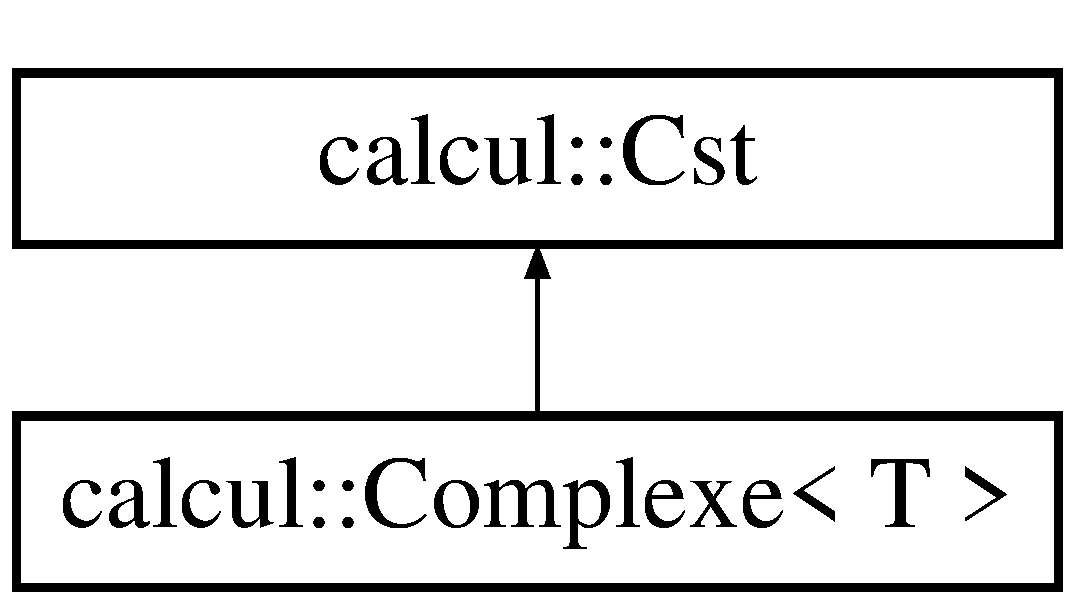
\includegraphics[height=2.000000cm]{classcalcul_1_1_complexe}
\end{center}
\end{figure}
\subsection*{Fonctions membres publiques}
\begin{DoxyCompactItemize}
\item 
\hypertarget{classcalcul_1_1_complexe_aaaceac3092c068cb9a47c368f072f233}{bool {\bfseries is\-Number} () const }\label{classcalcul_1_1_complexe_aaaceac3092c068cb9a47c368f072f233}

\item 
\hypertarget{classcalcul_1_1_complexe_ad37d17f91ebe787d4f19ab451200c7e0}{{\bfseries Complexe} (const T \&re=T(), const T \&img=T())}\label{classcalcul_1_1_complexe_ad37d17f91ebe787d4f19ab451200c7e0}

\item 
\hypertarget{classcalcul_1_1_complexe_aa0cc9d9fa0457a719a452758ffbb105c}{\hyperlink{classcalcul_1_1_complexe}{Complexe}$<$ T $>$ \& {\bfseries operator+} (const \hyperlink{classcalcul_1_1_cst}{Cst} \&other) const }\label{classcalcul_1_1_complexe_aa0cc9d9fa0457a719a452758ffbb105c}

\item 
\hypertarget{classcalcul_1_1_complexe_ad4d85ff5336cb7cc292688c04fb4bccd}{\hyperlink{classcalcul_1_1_complexe}{Complexe}$<$ T $>$ \& {\bfseries operator$\ast$} (const \hyperlink{classcalcul_1_1_cst}{Cst} \&other) const }\label{classcalcul_1_1_complexe_ad4d85ff5336cb7cc292688c04fb4bccd}

\item 
\hypertarget{classcalcul_1_1_complexe_abf3f2f71cc9914634a69afe681a67a25}{\hyperlink{classcalcul_1_1_complexe}{Complexe}$<$ T $>$ \& {\bfseries operator-\/} (const \hyperlink{classcalcul_1_1_cst}{Cst} \&other) const }\label{classcalcul_1_1_complexe_abf3f2f71cc9914634a69afe681a67a25}

\item 
\hypertarget{classcalcul_1_1_complexe_ac24e53f143838aff4063fdfbc9255bba}{\hyperlink{classcalcul_1_1_complexe}{Complexe}$<$ T $>$ \& {\bfseries operator/} (const \hyperlink{classcalcul_1_1_cst}{Cst} \&other) const }\label{classcalcul_1_1_complexe_ac24e53f143838aff4063fdfbc9255bba}

\item 
\hypertarget{classcalcul_1_1_complexe_a643bd98fc0db34fa8c1f665d2f8ff8f3}{\hyperlink{classcalcul_1_1_complexe}{Complexe}$<$ T $>$ \& {\bfseries M\-O\-D} (const \hyperlink{classcalcul_1_1_cst}{Cst} \&other) const }\label{classcalcul_1_1_complexe_a643bd98fc0db34fa8c1f665d2f8ff8f3}

\item 
\hypertarget{classcalcul_1_1_complexe_ad44ec7c707a729cad112a10a89bf7116}{\hyperlink{classcalcul_1_1_complexe}{Complexe}$<$ T $>$ \& {\bfseries P\-O\-W} (const \hyperlink{classcalcul_1_1_cst}{Cst} \&other) const }\label{classcalcul_1_1_complexe_ad44ec7c707a729cad112a10a89bf7116}

\item 
\hypertarget{classcalcul_1_1_complexe_aec629e64332eecd04f4c276b349d686a}{\hyperlink{classcalcul_1_1_complexe}{Complexe}$<$ T $>$ \& {\bfseries S\-Q\-R} () const }\label{classcalcul_1_1_complexe_aec629e64332eecd04f4c276b349d686a}

\item 
\hypertarget{classcalcul_1_1_complexe_ab121065d27b0b1001183cda196a0b300}{\hyperlink{classcalcul_1_1_complexe}{Complexe}$<$ T $>$ \& {\bfseries C\-U\-B\-E} () const }\label{classcalcul_1_1_complexe_ab121065d27b0b1001183cda196a0b300}

\item 
\hypertarget{classcalcul_1_1_complexe_ac662ebd095aaff0758fd9206986530c5}{\hyperlink{classcalcul_1_1_complexe}{Complexe}$<$ T $>$ \& {\bfseries S\-I\-G\-N} () const }\label{classcalcul_1_1_complexe_ac662ebd095aaff0758fd9206986530c5}

\item 
\hypertarget{classcalcul_1_1_complexe_a8cb370c02a514564de84e9e693ae4ac7}{\hyperlink{classcalcul_1_1_complexe}{Complexe}$<$ T $>$ \& {\bfseries S\-I\-N} (Angle\-Type angle=Degre) const }\label{classcalcul_1_1_complexe_a8cb370c02a514564de84e9e693ae4ac7}

\item 
\hypertarget{classcalcul_1_1_complexe_ad0e4743116f56f985a84e3cd51f6efe1}{\hyperlink{classcalcul_1_1_complexe}{Complexe}$<$ T $>$ \& {\bfseries C\-O\-S} (Angle\-Type angle=Degre) const }\label{classcalcul_1_1_complexe_ad0e4743116f56f985a84e3cd51f6efe1}

\item 
\hypertarget{classcalcul_1_1_complexe_aa828d019770a344aca27d95aa1d22ca9}{\hyperlink{classcalcul_1_1_complexe}{Complexe}$<$ T $>$ \& {\bfseries T\-A\-N} (Angle\-Type angle=Degre) const }\label{classcalcul_1_1_complexe_aa828d019770a344aca27d95aa1d22ca9}

\item 
\hypertarget{classcalcul_1_1_complexe_a09c8357113fc2ccee4892b282fc4ffc7}{\hyperlink{classcalcul_1_1_complexe}{Complexe}$<$ T $>$ \& {\bfseries S\-I\-N\-H} () const }\label{classcalcul_1_1_complexe_a09c8357113fc2ccee4892b282fc4ffc7}

\item 
\hypertarget{classcalcul_1_1_complexe_aa33b36c834307c44c6bf512e09c03c00}{\hyperlink{classcalcul_1_1_complexe}{Complexe}$<$ T $>$ \& {\bfseries C\-O\-S\-H} () const }\label{classcalcul_1_1_complexe_aa33b36c834307c44c6bf512e09c03c00}

\item 
\hypertarget{classcalcul_1_1_complexe_a6dd913302dc2ea8647a03b71ddbb383e}{\hyperlink{classcalcul_1_1_complexe}{Complexe}$<$ T $>$ \& {\bfseries T\-A\-N\-H} () const }\label{classcalcul_1_1_complexe_a6dd913302dc2ea8647a03b71ddbb383e}

\item 
\hypertarget{classcalcul_1_1_complexe_a641205a4acb7d56e32ffe2d85fa9467d}{\hyperlink{classcalcul_1_1_complexe}{Complexe}$<$ T $>$ \& {\bfseries L\-N} () const }\label{classcalcul_1_1_complexe_a641205a4acb7d56e32ffe2d85fa9467d}

\item 
\hypertarget{classcalcul_1_1_complexe_ac720ec3de9cf7aa71d3e6ebfded5e858}{\hyperlink{classcalcul_1_1_complexe}{Complexe}$<$ T $>$ \& {\bfseries L\-O\-G} () const }\label{classcalcul_1_1_complexe_ac720ec3de9cf7aa71d3e6ebfded5e858}

\item 
\hypertarget{classcalcul_1_1_complexe_a1973cc591dcff1f8ec2e632242f09e38}{\hyperlink{classcalcul_1_1_complexe}{Complexe}$<$ T $>$ \& {\bfseries I\-N\-V} () const }\label{classcalcul_1_1_complexe_a1973cc591dcff1f8ec2e632242f09e38}

\item 
\hypertarget{classcalcul_1_1_complexe_a6a4544daeb5c79750285dd1e92955b0d}{\hyperlink{classcalcul_1_1_complexe}{Complexe}$<$ T $>$ \& {\bfseries S\-Q\-R\-T} () const }\label{classcalcul_1_1_complexe_a6a4544daeb5c79750285dd1e92955b0d}

\item 
\hypertarget{classcalcul_1_1_complexe_a085dadb4042154e26d04b1f4b9bcd990}{\hyperlink{classcalcul_1_1_complexe}{Complexe}$<$ T $>$ \& {\bfseries F\-A\-C\-T} () const }\label{classcalcul_1_1_complexe_a085dadb4042154e26d04b1f4b9bcd990}

\item 
\hypertarget{classcalcul_1_1_complexe_ab972738348ad3181a35cd88a4bcc7c68}{\hyperlink{classcalcul_1_1_complexe}{Complexe}$<$ T $>$ \& {\bfseries E\-V\-A\-L} () const }\label{classcalcul_1_1_complexe_ab972738348ad3181a35cd88a4bcc7c68}

\end{DoxyCompactItemize}
\subsection*{Fonctions membres protégées}
\begin{DoxyCompactItemize}
\item 
\hypertarget{classcalcul_1_1_complexe_aafcfaebf5bb3e6b9bb89766832429efc}{void {\bfseries set\-String} ()}\label{classcalcul_1_1_complexe_aafcfaebf5bb3e6b9bb89766832429efc}

\end{DoxyCompactItemize}
\subsection*{Additional Inherited Members}


\subsection{Description détaillée}
\subsubsection*{template$<$class T$>$class calcul\-::\-Complexe$<$ T $>$}

Classe \hyperlink{classcalcul_1_1_complexe}{Complexe} implémentée avec une template. 

La documentation de cette classe a été générée à partir du fichier suivant \-:\begin{DoxyCompactItemize}
\item 
C\-:/\-Users/\-William/\-Dropbox/lo21/projet/\-Projet/cst.\-h\end{DoxyCompactItemize}

\hypertarget{classcalcul_1_1_cst}{\section{Référence de la classe calcul\-:\-:Cst}
\label{classcalcul_1_1_cst}\index{calcul\-::\-Cst@{calcul\-::\-Cst}}
}


Classe abstraite representant les constantes.  




{\ttfamily \#include $<$cst.\-h$>$}

Graphe d'héritage de calcul\-:\-:Cst\-:\begin{figure}[H]
\begin{center}
\leavevmode
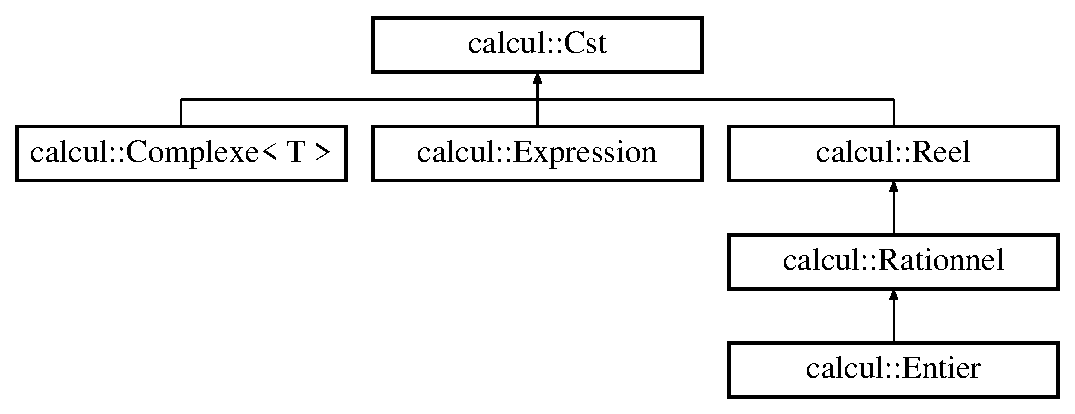
\includegraphics[height=4.000000cm]{classcalcul_1_1_cst}
\end{center}
\end{figure}
\subsection*{Fonctions membres publiques}
\begin{DoxyCompactItemize}
\item 
\hypertarget{classcalcul_1_1_cst_aad9a62f89cf706a578e8c91f8a3e5ee4}{Q\-String {\bfseries get\-String} () const }\label{classcalcul_1_1_cst_aad9a62f89cf706a578e8c91f8a3e5ee4}

\item 
\hypertarget{classcalcul_1_1_cst_ae38302c6557f87441ba299bc04a3845d}{virtual bool {\bfseries is\-Number} () const =0}\label{classcalcul_1_1_cst_ae38302c6557f87441ba299bc04a3845d}

\item 
\hypertarget{classcalcul_1_1_cst_ac0c0bee65b80528f5b97a3ab12baeff5}{virtual double {\bfseries get\-Valeur} () const }\label{classcalcul_1_1_cst_ac0c0bee65b80528f5b97a3ab12baeff5}

\item 
\hypertarget{classcalcul_1_1_cst_a1047aa48fd66af061463464989c9fab8}{virtual int {\bfseries get\-Num} () const }\label{classcalcul_1_1_cst_a1047aa48fd66af061463464989c9fab8}

\item 
\hypertarget{classcalcul_1_1_cst_ae97edda2c50631d45e448fa16ab9fe86}{virtual int {\bfseries get\-Den} () const }\label{classcalcul_1_1_cst_ae97edda2c50631d45e448fa16ab9fe86}

\item 
\hypertarget{classcalcul_1_1_cst_aa81b86f1f4c1206d653ec3ad3733a9ab}{virtual \hyperlink{classcalcul_1_1_cst}{Cst} \& {\bfseries operator+} (const \hyperlink{classcalcul_1_1_cst}{Cst} \&other) const =0}\label{classcalcul_1_1_cst_aa81b86f1f4c1206d653ec3ad3733a9ab}

\item 
\hypertarget{classcalcul_1_1_cst_a141745da396751c6a2ff012774fa1e74}{virtual \hyperlink{classcalcul_1_1_cst}{Cst} \& {\bfseries operator$\ast$} (const \hyperlink{classcalcul_1_1_cst}{Cst} \&other) const =0}\label{classcalcul_1_1_cst_a141745da396751c6a2ff012774fa1e74}

\item 
\hypertarget{classcalcul_1_1_cst_a4451f0f4ce0e47ee7ee1ae6c8634065f}{virtual \hyperlink{classcalcul_1_1_cst}{Cst} \& {\bfseries operator-\/} (const \hyperlink{classcalcul_1_1_cst}{Cst} \&other) const =0}\label{classcalcul_1_1_cst_a4451f0f4ce0e47ee7ee1ae6c8634065f}

\item 
\hypertarget{classcalcul_1_1_cst_aff0c1e1b70e53fb617861983730c07ff}{virtual \hyperlink{classcalcul_1_1_cst}{Cst} \& {\bfseries operator/} (const \hyperlink{classcalcul_1_1_cst}{Cst} \&other) const =0}\label{classcalcul_1_1_cst_aff0c1e1b70e53fb617861983730c07ff}

\item 
\hypertarget{classcalcul_1_1_cst_a6d682c73fab890843b1ca2fe6f52c031}{virtual \hyperlink{classcalcul_1_1_cst}{Cst} \& {\bfseries P\-O\-W} (const \hyperlink{classcalcul_1_1_cst}{Cst} \&other) const =0}\label{classcalcul_1_1_cst_a6d682c73fab890843b1ca2fe6f52c031}

\item 
\hypertarget{classcalcul_1_1_cst_ac5ec99196eb483ea7002b21d587b37f4}{virtual \hyperlink{classcalcul_1_1_cst}{Cst} \& {\bfseries M\-O\-D} (const \hyperlink{classcalcul_1_1_cst}{Cst} \&other) const =0}\label{classcalcul_1_1_cst_ac5ec99196eb483ea7002b21d587b37f4}

\item 
\hypertarget{classcalcul_1_1_cst_add103ef84aa3c58fcf3fe62f36473e87}{virtual \hyperlink{classcalcul_1_1_cst}{Cst} \& {\bfseries S\-Q\-R} () const =0}\label{classcalcul_1_1_cst_add103ef84aa3c58fcf3fe62f36473e87}

\item 
\hypertarget{classcalcul_1_1_cst_aac65269af13a78677d25af8513e89892}{virtual \hyperlink{classcalcul_1_1_cst}{Cst} \& {\bfseries C\-U\-B\-E} () const =0}\label{classcalcul_1_1_cst_aac65269af13a78677d25af8513e89892}

\item 
\hypertarget{classcalcul_1_1_cst_ae1ef0d7b1702ec42daa2c48ce0317bcc}{virtual \hyperlink{classcalcul_1_1_cst}{Cst} \& {\bfseries S\-I\-G\-N} () const =0}\label{classcalcul_1_1_cst_ae1ef0d7b1702ec42daa2c48ce0317bcc}

\item 
\hypertarget{classcalcul_1_1_cst_a9eee774878d7999497f9ae5bed62d50e}{virtual \hyperlink{classcalcul_1_1_cst}{Cst} \& {\bfseries S\-I\-N} (Angle\-Type angle=Degre) const =0}\label{classcalcul_1_1_cst_a9eee774878d7999497f9ae5bed62d50e}

\item 
\hypertarget{classcalcul_1_1_cst_a5d1586652f8785e0205d5dc4709605f1}{virtual \hyperlink{classcalcul_1_1_cst}{Cst} \& {\bfseries C\-O\-S} (Angle\-Type angle=Degre) const =0}\label{classcalcul_1_1_cst_a5d1586652f8785e0205d5dc4709605f1}

\item 
\hypertarget{classcalcul_1_1_cst_aafa0aa31332b8e4ea10e311325144109}{virtual \hyperlink{classcalcul_1_1_cst}{Cst} \& {\bfseries T\-A\-N} (Angle\-Type angle=Degre) const =0}\label{classcalcul_1_1_cst_aafa0aa31332b8e4ea10e311325144109}

\item 
\hypertarget{classcalcul_1_1_cst_abacebfb539c257bd9f5cf444291974c2}{virtual \hyperlink{classcalcul_1_1_cst}{Cst} \& {\bfseries S\-I\-N\-H} () const =0}\label{classcalcul_1_1_cst_abacebfb539c257bd9f5cf444291974c2}

\item 
\hypertarget{classcalcul_1_1_cst_ab8735cea23619305a409355101395816}{virtual \hyperlink{classcalcul_1_1_cst}{Cst} \& {\bfseries C\-O\-S\-H} () const =0}\label{classcalcul_1_1_cst_ab8735cea23619305a409355101395816}

\item 
\hypertarget{classcalcul_1_1_cst_af7e77e3fe63d0bbdbe16f9a828ac759a}{virtual \hyperlink{classcalcul_1_1_cst}{Cst} \& {\bfseries T\-A\-N\-H} () const =0}\label{classcalcul_1_1_cst_af7e77e3fe63d0bbdbe16f9a828ac759a}

\item 
\hypertarget{classcalcul_1_1_cst_a1d445a93dda3e4288da2041ee9dc1d26}{virtual \hyperlink{classcalcul_1_1_cst}{Cst} \& {\bfseries L\-N} () const =0}\label{classcalcul_1_1_cst_a1d445a93dda3e4288da2041ee9dc1d26}

\item 
\hypertarget{classcalcul_1_1_cst_adf79c329057724990d026991eb54cfb1}{virtual \hyperlink{classcalcul_1_1_cst}{Cst} \& {\bfseries L\-O\-G} () const =0}\label{classcalcul_1_1_cst_adf79c329057724990d026991eb54cfb1}

\item 
\hypertarget{classcalcul_1_1_cst_acd576258760b0450a830667ee297b2f7}{virtual \hyperlink{classcalcul_1_1_cst}{Cst} \& {\bfseries S\-Q\-R\-T} () const =0}\label{classcalcul_1_1_cst_acd576258760b0450a830667ee297b2f7}

\item 
\hypertarget{classcalcul_1_1_cst_aa9cc867144c699ee56f0f611ed08c4f7}{virtual \hyperlink{classcalcul_1_1_cst}{Cst} \& {\bfseries I\-N\-V} () const =0}\label{classcalcul_1_1_cst_aa9cc867144c699ee56f0f611ed08c4f7}

\item 
\hypertarget{classcalcul_1_1_cst_ab2a67e0b8e5e8124d342820f9fe2a2fa}{virtual \hyperlink{classcalcul_1_1_cst}{Cst} \& {\bfseries F\-A\-C\-T} () const =0}\label{classcalcul_1_1_cst_ab2a67e0b8e5e8124d342820f9fe2a2fa}

\item 
\hypertarget{classcalcul_1_1_cst_a067512ccbf4141bc826c9cffbb8f92f4}{virtual \hyperlink{classcalcul_1_1_cst}{Cst} \& {\bfseries E\-V\-A\-L} () const =0}\label{classcalcul_1_1_cst_a067512ccbf4141bc826c9cffbb8f92f4}

\end{DoxyCompactItemize}
\subsection*{Fonctions membres protégées}
\begin{DoxyCompactItemize}
\item 
\hypertarget{classcalcul_1_1_cst_aaad16363b75e0ae319b6a17bf0e53e44}{virtual void {\bfseries set\-String} ()=0}\label{classcalcul_1_1_cst_aaad16363b75e0ae319b6a17bf0e53e44}

\end{DoxyCompactItemize}
\subsection*{Attributs protégés}
\begin{DoxyCompactItemize}
\item 
\hypertarget{classcalcul_1_1_cst_ad4c38adf792d80b3a5c484ab382e6906}{Q\-String {\bfseries string\-\_\-associe}}\label{classcalcul_1_1_cst_ad4c38adf792d80b3a5c484ab382e6906}

\end{DoxyCompactItemize}


\subsection{Description détaillée}
Classe abstraite representant les constantes. 

La documentation de cette classe a été générée à partir du fichier suivant \-:\begin{DoxyCompactItemize}
\item 
C\-:/\-Users/\-William/\-Dropbox/lo21/projet/\-Projet/cst.\-h\end{DoxyCompactItemize}

\hypertarget{classcalcul_1_1_entier}{\section{Référence de la classe calcul\-:\-:Entier}
\label{classcalcul_1_1_entier}\index{calcul\-::\-Entier@{calcul\-::\-Entier}}
}


Classe \hyperlink{classcalcul_1_1_entier}{Entier} représentant toutes les constantes entières, hérite de la classe \hyperlink{classcalcul_1_1_rationnel}{Rationnel}.  




{\ttfamily \#include $<$cst.\-h$>$}

Graphe d'héritage de calcul\-:\-:Entier\-:\begin{figure}[H]
\begin{center}
\leavevmode
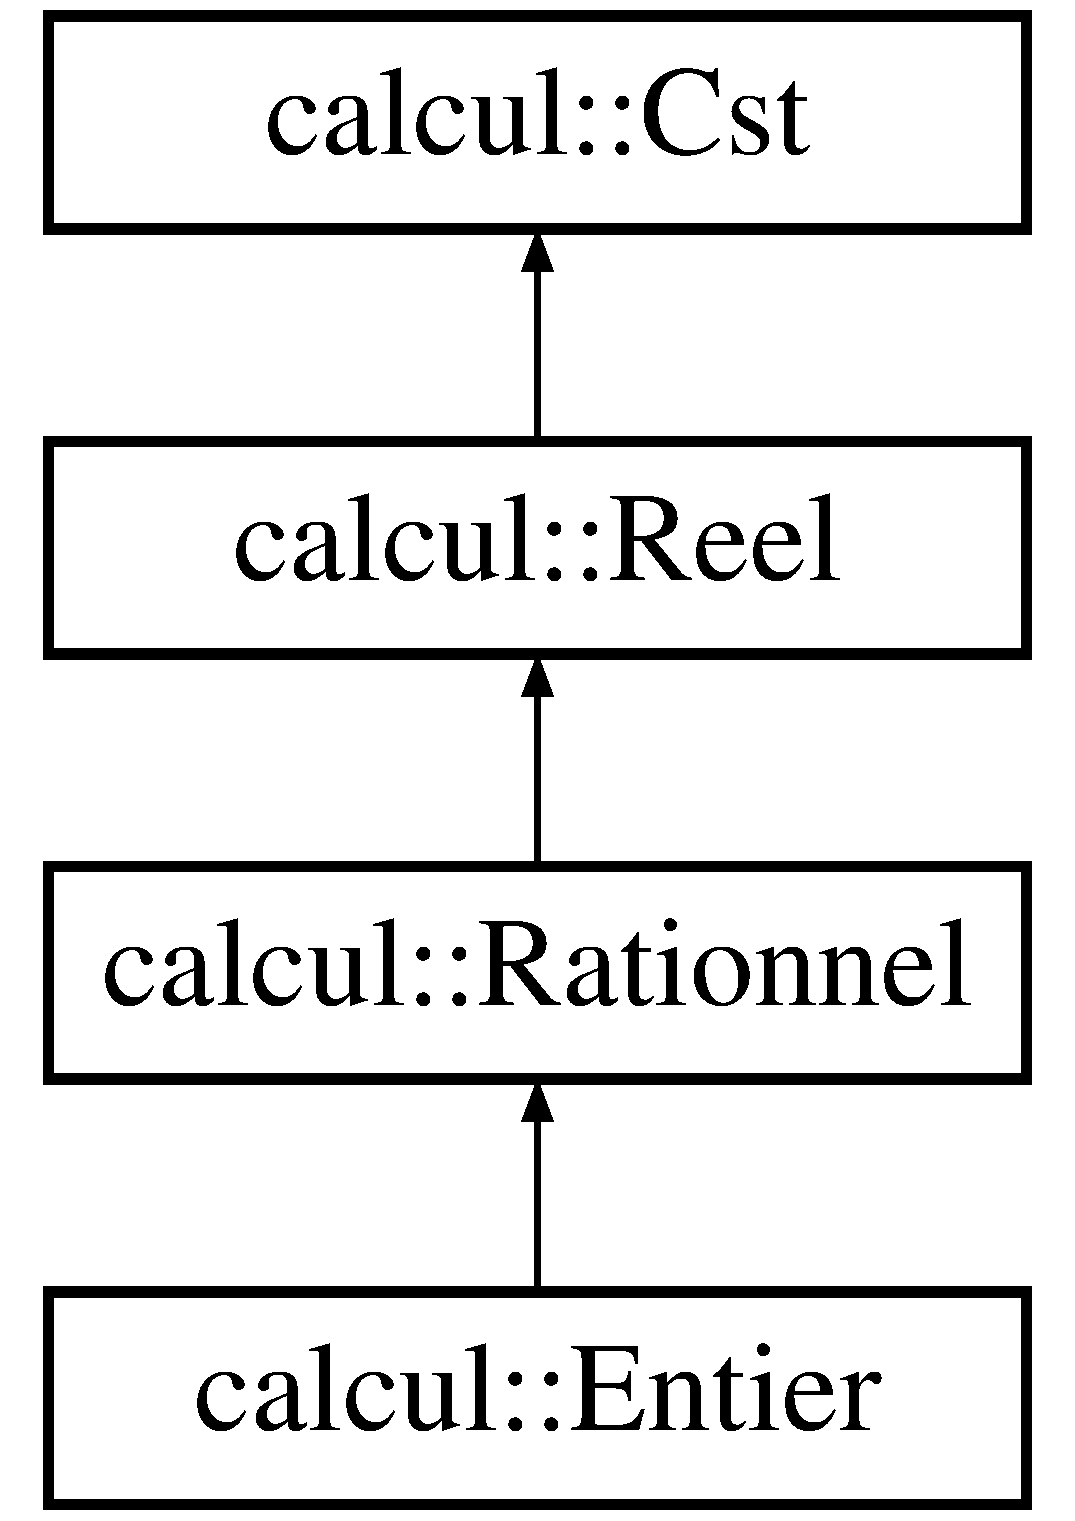
\includegraphics[height=4.000000cm]{classcalcul_1_1_entier}
\end{center}
\end{figure}
\subsection*{Fonctions membres publiques}
\begin{DoxyCompactItemize}
\item 
\hyperlink{classcalcul_1_1_entier_a9840d099d4b5b3f805699b5ba1a6eb3d}{Entier} (int valeur=0)
\begin{DoxyCompactList}\small\item\em Constructeur par défaut de la classe \hyperlink{classcalcul_1_1_entier}{Entier}. \end{DoxyCompactList}\item 
\hyperlink{classcalcul_1_1_entier_adfcff04f9903ae285a881621e6764903}{Entier} (const \hyperlink{classcalcul_1_1_cst}{Cst} \&a\-\_\-copier)
\begin{DoxyCompactList}\small\item\em Constructeur de recopie de la classe \hyperlink{classcalcul_1_1_entier}{Entier}. \end{DoxyCompactList}\item 
\hypertarget{classcalcul_1_1_entier_ac8a907eed01ccda92b6849e5f7895152}{\hyperlink{classcalcul_1_1_entier}{Entier} \& {\bfseries operator+} (const \hyperlink{classcalcul_1_1_cst}{Cst} \&other) const }\label{classcalcul_1_1_entier_ac8a907eed01ccda92b6849e5f7895152}

\item 
\hypertarget{classcalcul_1_1_entier_a78d5677a8ca7fd28eb54e4613b4c4c88}{\hyperlink{classcalcul_1_1_entier}{Entier} \& {\bfseries operator$\ast$} (const \hyperlink{classcalcul_1_1_cst}{Cst} \&other) const }\label{classcalcul_1_1_entier_a78d5677a8ca7fd28eb54e4613b4c4c88}

\item 
\hypertarget{classcalcul_1_1_entier_a7f19b05e1ba5df1d085aef46aa3fac10}{\hyperlink{classcalcul_1_1_entier}{Entier} \& {\bfseries operator-\/} (const \hyperlink{classcalcul_1_1_cst}{Cst} \&other) const }\label{classcalcul_1_1_entier_a7f19b05e1ba5df1d085aef46aa3fac10}

\item 
\hypertarget{classcalcul_1_1_entier_aae20e2ec9bf487e40c632bbcc76298f4}{\hyperlink{classcalcul_1_1_entier}{Entier} \& {\bfseries operator/} (const \hyperlink{classcalcul_1_1_cst}{Cst} \&other) const }\label{classcalcul_1_1_entier_aae20e2ec9bf487e40c632bbcc76298f4}

\item 
\hypertarget{classcalcul_1_1_entier_a07487e904c41b67b2516def34c2d7819}{\hyperlink{classcalcul_1_1_entier}{Entier} \& {\bfseries P\-O\-W} (const \hyperlink{classcalcul_1_1_cst}{Cst} \&other) const }\label{classcalcul_1_1_entier_a07487e904c41b67b2516def34c2d7819}

\item 
\hypertarget{classcalcul_1_1_entier_a9593983912ebb7497240b505b36c2422}{\hyperlink{classcalcul_1_1_entier}{Entier} \& {\bfseries M\-O\-D} (const \hyperlink{classcalcul_1_1_cst}{Cst} \&other) const }\label{classcalcul_1_1_entier_a9593983912ebb7497240b505b36c2422}

\item 
\hypertarget{classcalcul_1_1_entier_a2f242ab6c8a5ac938bd1b9af5c731e2f}{\hyperlink{classcalcul_1_1_entier}{Entier} \& {\bfseries S\-Q\-R} () const }\label{classcalcul_1_1_entier_a2f242ab6c8a5ac938bd1b9af5c731e2f}

\item 
\hypertarget{classcalcul_1_1_entier_a6b434e81d2165dfeaf76f4730c74e730}{\hyperlink{classcalcul_1_1_entier}{Entier} \& {\bfseries C\-U\-B\-E} () const }\label{classcalcul_1_1_entier_a6b434e81d2165dfeaf76f4730c74e730}

\item 
\hypertarget{classcalcul_1_1_entier_ac6063b81909893ca4bf587aff94cd5e9}{\hyperlink{classcalcul_1_1_entier}{Entier} \& {\bfseries S\-I\-G\-N} () const }\label{classcalcul_1_1_entier_ac6063b81909893ca4bf587aff94cd5e9}

\item 
\hypertarget{classcalcul_1_1_entier_addac1459c3b0491852ca47b9055ea00e}{\hyperlink{classcalcul_1_1_entier}{Entier} \& {\bfseries S\-I\-N} (Angle\-Type angle=Degre) const }\label{classcalcul_1_1_entier_addac1459c3b0491852ca47b9055ea00e}

\item 
\hypertarget{classcalcul_1_1_entier_a9e69913d43da7c2e0986f1a2e8d95341}{\hyperlink{classcalcul_1_1_entier}{Entier} \& {\bfseries C\-O\-S} (Angle\-Type angle=Degre) const }\label{classcalcul_1_1_entier_a9e69913d43da7c2e0986f1a2e8d95341}

\item 
\hypertarget{classcalcul_1_1_entier_add24dbddeefc055418702840c4b49340}{\hyperlink{classcalcul_1_1_entier}{Entier} \& {\bfseries T\-A\-N} (Angle\-Type angle=Degre) const }\label{classcalcul_1_1_entier_add24dbddeefc055418702840c4b49340}

\item 
\hypertarget{classcalcul_1_1_entier_a182214f92252e4f3be8b8f9fdd160bdd}{\hyperlink{classcalcul_1_1_entier}{Entier} \& {\bfseries S\-I\-N\-H} () const }\label{classcalcul_1_1_entier_a182214f92252e4f3be8b8f9fdd160bdd}

\item 
\hypertarget{classcalcul_1_1_entier_aefdd9b0da080254cf85c85d900aace78}{\hyperlink{classcalcul_1_1_entier}{Entier} \& {\bfseries C\-O\-S\-H} () const }\label{classcalcul_1_1_entier_aefdd9b0da080254cf85c85d900aace78}

\item 
\hypertarget{classcalcul_1_1_entier_a93405672bba677f91549e9493fc4b73e}{\hyperlink{classcalcul_1_1_entier}{Entier} \& {\bfseries T\-A\-N\-H} () const }\label{classcalcul_1_1_entier_a93405672bba677f91549e9493fc4b73e}

\item 
\hypertarget{classcalcul_1_1_entier_ae60d95379e527abecf9d3f64d5b81b15}{\hyperlink{classcalcul_1_1_entier}{Entier} \& {\bfseries L\-N} () const }\label{classcalcul_1_1_entier_ae60d95379e527abecf9d3f64d5b81b15}

\item 
\hypertarget{classcalcul_1_1_entier_a80193288132a92af48fdf6d2fe73291a}{\hyperlink{classcalcul_1_1_entier}{Entier} \& {\bfseries L\-O\-G} () const }\label{classcalcul_1_1_entier_a80193288132a92af48fdf6d2fe73291a}

\item 
\hypertarget{classcalcul_1_1_entier_a8edab0b60f0f0603a433b60b351131a4}{\hyperlink{classcalcul_1_1_entier}{Entier} \& {\bfseries S\-Q\-R\-T} () const }\label{classcalcul_1_1_entier_a8edab0b60f0f0603a433b60b351131a4}

\item 
\hypertarget{classcalcul_1_1_entier_a2c4f45ee53d7d4172fdd793a90256864}{\hyperlink{classcalcul_1_1_entier}{Entier} \& {\bfseries I\-N\-V} () const }\label{classcalcul_1_1_entier_a2c4f45ee53d7d4172fdd793a90256864}

\item 
\hypertarget{classcalcul_1_1_entier_a5b79ae6de2447c5abd72e87e063631aa}{\hyperlink{classcalcul_1_1_entier}{Entier} \& {\bfseries F\-A\-C\-T} () const }\label{classcalcul_1_1_entier_a5b79ae6de2447c5abd72e87e063631aa}

\item 
\hypertarget{classcalcul_1_1_entier_a8b9152f7b127161bfa1070c84799656c}{\hyperlink{classcalcul_1_1_entier}{Entier} \& {\bfseries E\-V\-A\-L} () const }\label{classcalcul_1_1_entier_a8b9152f7b127161bfa1070c84799656c}

\end{DoxyCompactItemize}
\subsection*{Additional Inherited Members}


\subsection{Description détaillée}
Classe \hyperlink{classcalcul_1_1_entier}{Entier} représentant toutes les constantes entières, hérite de la classe \hyperlink{classcalcul_1_1_rationnel}{Rationnel}. 

\subsection{Documentation des constructeurs et destructeur}
\hypertarget{classcalcul_1_1_entier_a9840d099d4b5b3f805699b5ba1a6eb3d}{\index{calcul\-::\-Entier@{calcul\-::\-Entier}!Entier@{Entier}}
\index{Entier@{Entier}!calcul::Entier@{calcul\-::\-Entier}}
\subsubsection[{Entier}]{\setlength{\rightskip}{0pt plus 5cm}calcul\-::\-Entier\-::\-Entier (
\begin{DoxyParamCaption}
\item[{int}]{valeur = {\ttfamily 0}}
\end{DoxyParamCaption}
)\hspace{0.3cm}{\ttfamily [inline]}}}\label{classcalcul_1_1_entier_a9840d099d4b5b3f805699b5ba1a6eb3d}


Constructeur par défaut de la classe \hyperlink{classcalcul_1_1_entier}{Entier}. 


\begin{DoxyParams}{Paramètres}
{\em valeur} & \-: Valeur de la constante \\
\hline
\end{DoxyParams}
\hypertarget{classcalcul_1_1_entier_adfcff04f9903ae285a881621e6764903}{\index{calcul\-::\-Entier@{calcul\-::\-Entier}!Entier@{Entier}}
\index{Entier@{Entier}!calcul::Entier@{calcul\-::\-Entier}}
\subsubsection[{Entier}]{\setlength{\rightskip}{0pt plus 5cm}calcul\-::\-Entier\-::\-Entier (
\begin{DoxyParamCaption}
\item[{const {\bf Cst} \&}]{a\-\_\-copier}
\end{DoxyParamCaption}
)\hspace{0.3cm}{\ttfamily [inline]}}}\label{classcalcul_1_1_entier_adfcff04f9903ae285a881621e6764903}


Constructeur de recopie de la classe \hyperlink{classcalcul_1_1_entier}{Entier}. 


\begin{DoxyParams}{Paramètres}
{\em a\-\_\-copier} & \-: La constante entière à recopier \\
\hline
\end{DoxyParams}


La documentation de cette classe a été générée à partir des fichiers suivants \-:\begin{DoxyCompactItemize}
\item 
C\-:/\-Users/\-William/\-Dropbox/lo21/projet/\-Projet/cst.\-h\item 
C\-:/\-Users/\-William/\-Dropbox/lo21/projet/\-Projet/cst.\-cpp\end{DoxyCompactItemize}

\hypertarget{class_onglet_1_1evenement}{\section{Référence de la classe Onglet\-:\-:evenement}
\label{class_onglet_1_1evenement}\index{Onglet\-::evenement@{Onglet\-::evenement}}
}


Classe interne pour traiter les évenements.  




{\ttfamily \#include $<$onglet.\-h$>$}

\subsection*{Fonctions membres publiques}
\begin{DoxyCompactItemize}
\item 
void \hyperlink{class_onglet_1_1evenement_af0fd82d8213ce1e7d0ca021eb8903888}{traitement} (Q\-String type\-Traitement, \hyperlink{class_onglet}{Onglet} $\ast$ong, Q\-Object $\ast$sender=0)
\begin{DoxyCompactList}\small\item\em Réagir selon l'action de l'utilisateur. \end{DoxyCompactList}\item 
\hypertarget{class_onglet_1_1evenement_a1c8815617f15cfe57a7c267edbd085ec}{void \hyperlink{class_onglet_1_1evenement_a1c8815617f15cfe57a7c267edbd085ec}{op\-Non\-Reels} (\hyperlink{class_onglet}{Onglet} $\ast$ong)}\label{class_onglet_1_1evenement_a1c8815617f15cfe57a7c267edbd085ec}

\begin{DoxyCompactList}\small\item\em Méthode qui désactive les boutons non-\/accessible aux réels. \end{DoxyCompactList}\item 
\hypertarget{class_onglet_1_1evenement_ad5ed69991e6e1a2b92c542f3e850e7a2}{void \hyperlink{class_onglet_1_1evenement_ad5ed69991e6e1a2b92c542f3e850e7a2}{op\-Non\-Complexes} (\hyperlink{class_onglet}{Onglet} $\ast$ong)}\label{class_onglet_1_1evenement_ad5ed69991e6e1a2b92c542f3e850e7a2}

\begin{DoxyCompactList}\small\item\em Méthode qui désactive les boutons non-\/accessible aux complexes. \end{DoxyCompactList}\item 
\hypertarget{class_onglet_1_1evenement_a6980506e8a68ec43501d7facf9cdc421}{void \hyperlink{class_onglet_1_1evenement_a6980506e8a68ec43501d7facf9cdc421}{op\-Non\-Rationels} (\hyperlink{class_onglet}{Onglet} $\ast$ong)}\label{class_onglet_1_1evenement_a6980506e8a68ec43501d7facf9cdc421}

\begin{DoxyCompactList}\small\item\em Méthode qui désactive les boutons non-\/accessible aux rationnels. \end{DoxyCompactList}\item 
\hypertarget{class_onglet_1_1evenement_ad4e0d8fdd75d44ce173443097d934fe5}{void \hyperlink{class_onglet_1_1evenement_ad4e0d8fdd75d44ce173443097d934fe5}{clavier\-Basic\-Visible} (bool visible, \hyperlink{class_onglet}{Onglet} $\ast$ong)}\label{class_onglet_1_1evenement_ad4e0d8fdd75d44ce173443097d934fe5}

\begin{DoxyCompactList}\small\item\em Méthode qui affiche ou cache le clavier basic. \end{DoxyCompactList}\item 
\hypertarget{class_onglet_1_1evenement_a8c074378bdc1f4165723b35a85ffe017}{void \hyperlink{class_onglet_1_1evenement_a8c074378bdc1f4165723b35a85ffe017}{clavier\-Avance\-Visible} (bool visible, \hyperlink{class_onglet}{Onglet} $\ast$ong)}\label{class_onglet_1_1evenement_a8c074378bdc1f4165723b35a85ffe017}

\begin{DoxyCompactList}\small\item\em Méthode qui affiche ou cache le clavier avancé \end{DoxyCompactList}\end{DoxyCompactItemize}


\subsection{Description détaillée}
Classe interne pour traiter les évenements. 

\subsection{Documentation des fonctions membres}
\hypertarget{class_onglet_1_1evenement_af0fd82d8213ce1e7d0ca021eb8903888}{\index{Onglet\-::evenement@{Onglet\-::evenement}!traitement@{traitement}}
\index{traitement@{traitement}!Onglet::evenement@{Onglet\-::evenement}}
\subsubsection[{traitement}]{\setlength{\rightskip}{0pt plus 5cm}void Onglet\-::evenement\-::traitement (
\begin{DoxyParamCaption}
\item[{Q\-String}]{type\-Traitement, }
\item[{{\bf Onglet} $\ast$}]{ong, }
\item[{Q\-Object $\ast$}]{sender = {\ttfamily 0}}
\end{DoxyParamCaption}
)}}\label{class_onglet_1_1evenement_af0fd82d8213ce1e7d0ca021eb8903888}


Réagir selon l'action de l'utilisateur. 


\begin{DoxyParams}{Paramètres}
{\em type\-Traitement} & \-: Type d'action \\
\hline
{\em ong} & \-: Pointeur sur l'onglet actuel \\
\hline
{\em sender} & \-: Le composant concerné \\
\hline
\end{DoxyParams}


La documentation de cette classe a été générée à partir des fichiers suivants \-:\begin{DoxyCompactItemize}
\item 
C\-:/\-Users/\-William/\-Dropbox/lo21/projet/\-Projet/onglet.\-h\item 
C\-:/\-Users/\-William/\-Dropbox/lo21/projet/\-Projet/onglet.\-cpp\end{DoxyCompactItemize}

\hypertarget{class_exception}{\section{Référence de la classe Exception}
\label{class_exception}\index{Exception@{Exception}}
}


La classe représentant une exception. On utilise exception sans throw, pour envoyer des messages ou des logs type \char`\"{}pertes de donnees pour un sinus d'entier\char`\"{}.  




{\ttfamily \#include $<$exception\-\_\-log.\-h$>$}

Graphe d'héritage de Exception\-:\begin{figure}[H]
\begin{center}
\leavevmode
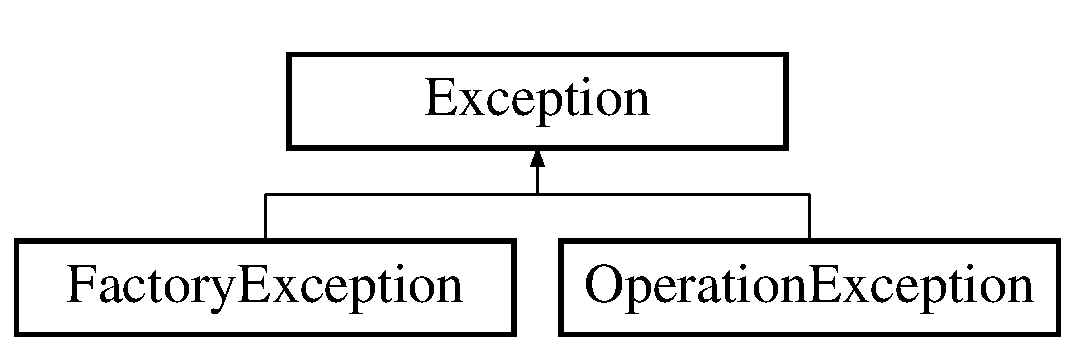
\includegraphics[height=2.000000cm]{class_exception}
\end{center}
\end{figure}
\subsection*{Fonctions membres publiques}
\begin{DoxyCompactItemize}
\item 
\hyperlink{class_exception_aebfa9ca3116e897aa52160793080cc29}{Exception} (Q\-String message)
\begin{DoxyCompactList}\small\item\em Constructeur de la classe \hyperlink{class_exception}{Exception}. \end{DoxyCompactList}\item 
Q\-String \hyperlink{class_exception_a20b6402f042207e125a9b3776b3c60c6}{get\-Message} () const 
\begin{DoxyCompactList}\small\item\em Récupérer le message de l'exception. \end{DoxyCompactList}\item 
\hypertarget{class_exception_a5874c51943108fae7f792b5a80673b86}{virtual const \hyperlink{class_exception}{Exception} \& \hyperlink{class_exception_a5874c51943108fae7f792b5a80673b86}{send\-Message} () const }\label{class_exception_a5874c51943108fae7f792b5a80673b86}

\begin{DoxyCompactList}\small\item\em Méthode virtual qui crée une boîte de diaglogue pour l'exception. \end{DoxyCompactList}\item 
\hypertarget{class_exception_a1a55a11a1379f03e15323c8015fb714e}{virtual const \hyperlink{class_exception}{Exception} \& \hyperlink{class_exception_a1a55a11a1379f03e15323c8015fb714e}{send\-Log} () const }\label{class_exception_a1a55a11a1379f03e15323c8015fb714e}

\begin{DoxyCompactList}\small\item\em Méthode virtual qui envoie le message d'exception au Logsysteme. \end{DoxyCompactList}\end{DoxyCompactItemize}
\subsection*{Attributs protégés}
\begin{DoxyCompactItemize}
\item 
\hypertarget{class_exception_a0ecd6018bc7499fe883e5ccedb142e19}{Q\-String {\bfseries message}}\label{class_exception_a0ecd6018bc7499fe883e5ccedb142e19}

\end{DoxyCompactItemize}


\subsection{Description détaillée}
La classe représentant une exception. On utilise exception sans throw, pour envoyer des messages ou des logs type \char`\"{}pertes de donnees pour un sinus d'entier\char`\"{}. 

\subsection{Documentation des constructeurs et destructeur}
\hypertarget{class_exception_aebfa9ca3116e897aa52160793080cc29}{\index{Exception@{Exception}!Exception@{Exception}}
\index{Exception@{Exception}!Exception@{Exception}}
\subsubsection[{Exception}]{\setlength{\rightskip}{0pt plus 5cm}Exception\-::\-Exception (
\begin{DoxyParamCaption}
\item[{Q\-String}]{message}
\end{DoxyParamCaption}
)\hspace{0.3cm}{\ttfamily [inline]}}}\label{class_exception_aebfa9ca3116e897aa52160793080cc29}


Constructeur de la classe \hyperlink{class_exception}{Exception}. 


\begin{DoxyParams}{Paramètres}
{\em message} & \-: Le message de l'exception \\
\hline
\end{DoxyParams}


\subsection{Documentation des fonctions membres}
\hypertarget{class_exception_a20b6402f042207e125a9b3776b3c60c6}{\index{Exception@{Exception}!get\-Message@{get\-Message}}
\index{get\-Message@{get\-Message}!Exception@{Exception}}
\subsubsection[{get\-Message}]{\setlength{\rightskip}{0pt plus 5cm}Q\-String Exception\-::get\-Message (
\begin{DoxyParamCaption}
{}
\end{DoxyParamCaption}
) const\hspace{0.3cm}{\ttfamily [inline]}}}\label{class_exception_a20b6402f042207e125a9b3776b3c60c6}


Récupérer le message de l'exception. 

\begin{DoxyReturn}{Renvoie}
Le message de l'exception 
\end{DoxyReturn}


La documentation de cette classe a été générée à partir du fichier suivant \-:\begin{DoxyCompactItemize}
\item 
C\-:/\-Users/\-William/\-Dropbox/lo21/projet/\-Projet/exception\-\_\-log.\-h\end{DoxyCompactItemize}

\hypertarget{classcalcul_1_1_expression}{\section{Référence de la classe calcul\-:\-:Expression}
\label{classcalcul_1_1_expression}\index{calcul\-::\-Expression@{calcul\-::\-Expression}}
}


Classe hérite de la classe \hyperlink{classcalcul_1_1_cst}{Cst} et représente une expression.  




{\ttfamily \#include $<$expression.\-h$>$}

Graphe d'héritage de calcul\-:\-:Expression\-:\begin{figure}[H]
\begin{center}
\leavevmode
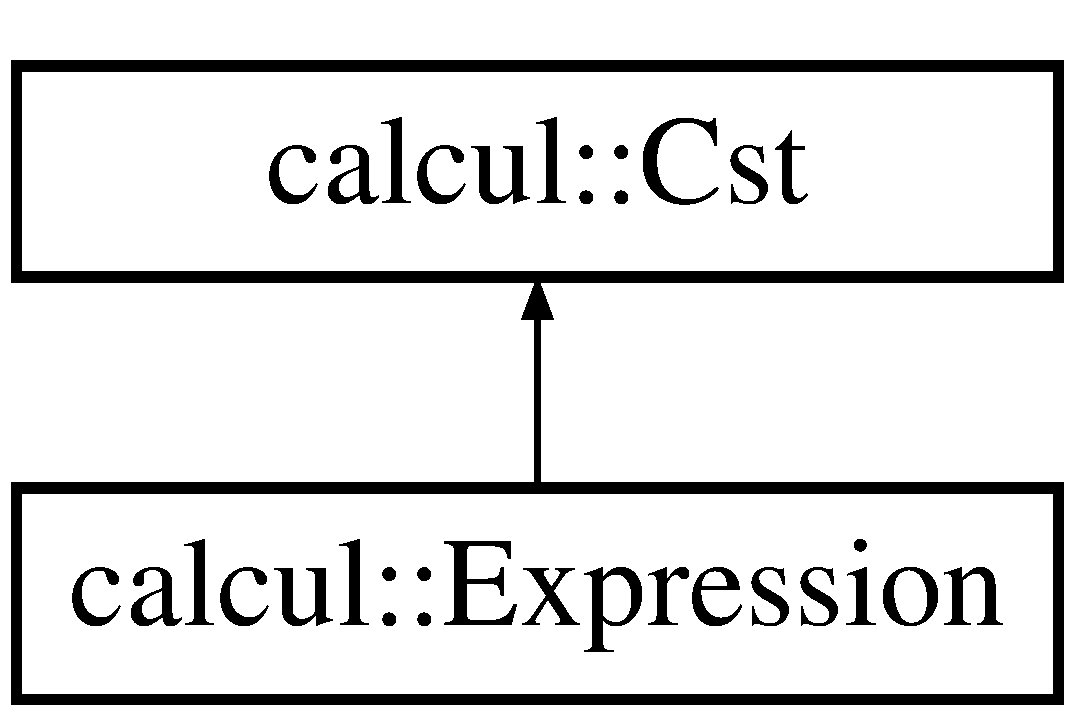
\includegraphics[height=2.000000cm]{classcalcul_1_1_expression}
\end{center}
\end{figure}
\subsection*{Fonctions membres publiques}
\begin{DoxyCompactItemize}
\item 
\hyperlink{classcalcul_1_1_expression_a85f5f40095d4be1fb44f703c6c854da0}{Expression} (Q\-String str)
\begin{DoxyCompactList}\small\item\em Constructeur de la classe \hyperlink{classcalcul_1_1_expression}{Expression}. \end{DoxyCompactList}\item 
bool \hyperlink{classcalcul_1_1_expression_a4b892bc1593c0717f90e085f1badd6d9}{is\-Number} () const 
\begin{DoxyCompactList}\small\item\em Vérifier si l'expression est un nombre. \end{DoxyCompactList}\item 
\hypertarget{classcalcul_1_1_expression_af04a22ee7ebb0c9d1b595904ffae62dc}{\hyperlink{classcalcul_1_1_expression}{Expression} \& {\bfseries operator+} (const \hyperlink{classcalcul_1_1_cst}{Cst} \&other) const }\label{classcalcul_1_1_expression_af04a22ee7ebb0c9d1b595904ffae62dc}

\item 
\hypertarget{classcalcul_1_1_expression_a1ec539865decac6220c7b7db3524d031}{\hyperlink{classcalcul_1_1_expression}{Expression} \& {\bfseries operator$\ast$} (const \hyperlink{classcalcul_1_1_cst}{Cst} \&other) const }\label{classcalcul_1_1_expression_a1ec539865decac6220c7b7db3524d031}

\item 
\hypertarget{classcalcul_1_1_expression_af0a2058ed6730e6b8c0e0d296e7d55fb}{\hyperlink{classcalcul_1_1_expression}{Expression} \& {\bfseries operator-\/} (const \hyperlink{classcalcul_1_1_cst}{Cst} \&other) const }\label{classcalcul_1_1_expression_af0a2058ed6730e6b8c0e0d296e7d55fb}

\item 
\hypertarget{classcalcul_1_1_expression_a0d747d1ecc7a36b244c78ff024549586}{\hyperlink{classcalcul_1_1_expression}{Expression} \& {\bfseries operator/} (const \hyperlink{classcalcul_1_1_cst}{Cst} \&other) const }\label{classcalcul_1_1_expression_a0d747d1ecc7a36b244c78ff024549586}

\item 
\hypertarget{classcalcul_1_1_expression_a21d0696df2897bafb91ca2d7161199c3}{\hyperlink{classcalcul_1_1_expression}{Expression} \& {\bfseries P\-O\-W} (const \hyperlink{classcalcul_1_1_cst}{Cst} \&other) const }\label{classcalcul_1_1_expression_a21d0696df2897bafb91ca2d7161199c3}

\item 
\hypertarget{classcalcul_1_1_expression_a1368b90a310abb213371ac041d5113ce}{\hyperlink{classcalcul_1_1_expression}{Expression} \& {\bfseries M\-O\-D} (const \hyperlink{classcalcul_1_1_cst}{Cst} \&other) const }\label{classcalcul_1_1_expression_a1368b90a310abb213371ac041d5113ce}

\item 
\hypertarget{classcalcul_1_1_expression_a18ff6a973911dbc04463557cdcaa28d8}{\hyperlink{classcalcul_1_1_expression}{Expression} \& {\bfseries S\-Q\-R} () const }\label{classcalcul_1_1_expression_a18ff6a973911dbc04463557cdcaa28d8}

\item 
\hypertarget{classcalcul_1_1_expression_a47fdb82fd3c81e2b5ead01017a99cb3c}{\hyperlink{classcalcul_1_1_expression}{Expression} \& {\bfseries C\-U\-B\-E} () const }\label{classcalcul_1_1_expression_a47fdb82fd3c81e2b5ead01017a99cb3c}

\item 
\hypertarget{classcalcul_1_1_expression_af395291cb886338fa71a3f654231bae5}{\hyperlink{classcalcul_1_1_expression}{Expression} \& {\bfseries S\-I\-G\-N} () const }\label{classcalcul_1_1_expression_af395291cb886338fa71a3f654231bae5}

\item 
\hypertarget{classcalcul_1_1_expression_a6d4779403c6308e4494e185c247eac78}{\hyperlink{classcalcul_1_1_expression}{Expression} \& {\bfseries S\-I\-N} (Angle\-Type angle=Degre) const }\label{classcalcul_1_1_expression_a6d4779403c6308e4494e185c247eac78}

\item 
\hypertarget{classcalcul_1_1_expression_a2bf236c0fb76f8a7e2f34aa6b7a5ea02}{\hyperlink{classcalcul_1_1_expression}{Expression} \& {\bfseries C\-O\-S} (Angle\-Type angle=Degre) const }\label{classcalcul_1_1_expression_a2bf236c0fb76f8a7e2f34aa6b7a5ea02}

\item 
\hypertarget{classcalcul_1_1_expression_acf4e2db3069bb1a746f9db2632ac8e48}{\hyperlink{classcalcul_1_1_expression}{Expression} \& {\bfseries T\-A\-N} (Angle\-Type angle=Degre) const }\label{classcalcul_1_1_expression_acf4e2db3069bb1a746f9db2632ac8e48}

\item 
\hypertarget{classcalcul_1_1_expression_ae2f4152066fccc59b7a061afcece283c}{\hyperlink{classcalcul_1_1_expression}{Expression} \& {\bfseries S\-I\-N\-H} () const }\label{classcalcul_1_1_expression_ae2f4152066fccc59b7a061afcece283c}

\item 
\hypertarget{classcalcul_1_1_expression_a0a702167b4476c8b05ecc0587fa63775}{\hyperlink{classcalcul_1_1_expression}{Expression} \& {\bfseries C\-O\-S\-H} () const }\label{classcalcul_1_1_expression_a0a702167b4476c8b05ecc0587fa63775}

\item 
\hypertarget{classcalcul_1_1_expression_aae9115c143603a131f95e3efc25b5c67}{\hyperlink{classcalcul_1_1_expression}{Expression} \& {\bfseries T\-A\-N\-H} () const }\label{classcalcul_1_1_expression_aae9115c143603a131f95e3efc25b5c67}

\item 
\hypertarget{classcalcul_1_1_expression_a06fe4c1848db73c7738d3f0284194a72}{\hyperlink{classcalcul_1_1_expression}{Expression} \& {\bfseries L\-N} () const }\label{classcalcul_1_1_expression_a06fe4c1848db73c7738d3f0284194a72}

\item 
\hypertarget{classcalcul_1_1_expression_a70768ab872d70d70415ecc46169776e9}{\hyperlink{classcalcul_1_1_expression}{Expression} \& {\bfseries L\-O\-G} () const }\label{classcalcul_1_1_expression_a70768ab872d70d70415ecc46169776e9}

\item 
\hypertarget{classcalcul_1_1_expression_afe619fd986a1153f5e1d134c915eb76b}{\hyperlink{classcalcul_1_1_expression}{Expression} \& {\bfseries S\-Q\-R\-T} () const }\label{classcalcul_1_1_expression_afe619fd986a1153f5e1d134c915eb76b}

\item 
\hypertarget{classcalcul_1_1_expression_a6545bd5b4ee6d444d75335e616587cec}{\hyperlink{classcalcul_1_1_expression}{Expression} \& {\bfseries I\-N\-V} () const }\label{classcalcul_1_1_expression_a6545bd5b4ee6d444d75335e616587cec}

\item 
\hypertarget{classcalcul_1_1_expression_a64e4b66b944faae6b1af22976a044047}{\hyperlink{classcalcul_1_1_expression}{Expression} \& {\bfseries F\-A\-C\-T} () const }\label{classcalcul_1_1_expression_a64e4b66b944faae6b1af22976a044047}

\item 
\hypertarget{classcalcul_1_1_expression_abf5174edfd7f2c2821e73d2e28d3e400}{\hyperlink{classcalcul_1_1_expression}{Expression} \& {\bfseries E\-V\-A\-L} () const }\label{classcalcul_1_1_expression_abf5174edfd7f2c2821e73d2e28d3e400}

\end{DoxyCompactItemize}
\subsection*{Fonctions membres protégées}
\begin{DoxyCompactItemize}
\item 
\hypertarget{classcalcul_1_1_expression_a20ad645dd608881832a65efcb42110a0}{void {\bfseries set\-String} ()}\label{classcalcul_1_1_expression_a20ad645dd608881832a65efcb42110a0}

\end{DoxyCompactItemize}
\subsection*{Additional Inherited Members}


\subsection{Description détaillée}
Classe hérite de la classe \hyperlink{classcalcul_1_1_cst}{Cst} et représente une expression. 

\subsection{Documentation des constructeurs et destructeur}
\hypertarget{classcalcul_1_1_expression_a85f5f40095d4be1fb44f703c6c854da0}{\index{calcul\-::\-Expression@{calcul\-::\-Expression}!Expression@{Expression}}
\index{Expression@{Expression}!calcul::Expression@{calcul\-::\-Expression}}
\subsubsection[{Expression}]{\setlength{\rightskip}{0pt plus 5cm}calcul\-::\-Expression\-::\-Expression (
\begin{DoxyParamCaption}
\item[{Q\-String}]{str}
\end{DoxyParamCaption}
)\hspace{0.3cm}{\ttfamily [inline]}}}\label{classcalcul_1_1_expression_a85f5f40095d4be1fb44f703c6c854da0}


Constructeur de la classe \hyperlink{classcalcul_1_1_expression}{Expression}. 


\begin{DoxyParams}{Paramètres}
{\em str} & \-: La chaîne de caractère à convertir en \hyperlink{classcalcul_1_1_expression}{Expression} \\
\hline
\end{DoxyParams}


\subsection{Documentation des fonctions membres}
\hypertarget{classcalcul_1_1_expression_a4b892bc1593c0717f90e085f1badd6d9}{\index{calcul\-::\-Expression@{calcul\-::\-Expression}!is\-Number@{is\-Number}}
\index{is\-Number@{is\-Number}!calcul::Expression@{calcul\-::\-Expression}}
\subsubsection[{is\-Number}]{\setlength{\rightskip}{0pt plus 5cm}bool calcul\-::\-Expression\-::is\-Number (
\begin{DoxyParamCaption}
{}
\end{DoxyParamCaption}
) const\hspace{0.3cm}{\ttfamily [inline]}, {\ttfamily [virtual]}}}\label{classcalcul_1_1_expression_a4b892bc1593c0717f90e085f1badd6d9}


Vérifier si l'expression est un nombre. 

\begin{DoxyReturn}{Renvoie}
True si l'expression est un nombre 
\end{DoxyReturn}


Implémente \hyperlink{classcalcul_1_1_cst}{calcul\-::\-Cst}.



La documentation de cette classe a été générée à partir des fichiers suivants \-:\begin{DoxyCompactItemize}
\item 
C\-:/\-Users/\-William/\-Dropbox/lo21/projet/\-Projet/expression.\-h\item 
C\-:/\-Users/\-William/\-Dropbox/lo21/projet/\-Projet/expression.\-cpp\end{DoxyCompactItemize}

\hypertarget{classcalcul_1_1_factory}{\section{Référence de la classe calcul\-:\-:Factory}
\label{classcalcul_1_1_factory}\index{calcul\-::\-Factory@{calcul\-::\-Factory}}
}


Classe abstraite implémentée en Design Pattern \hyperlink{classcalcul_1_1_factory}{Factory} Method pour créer des constantes.  




{\ttfamily \#include $<$factory.\-h$>$}

Graphe d'héritage de calcul\-:\-:Factory\-:\begin{figure}[H]
\begin{center}
\leavevmode
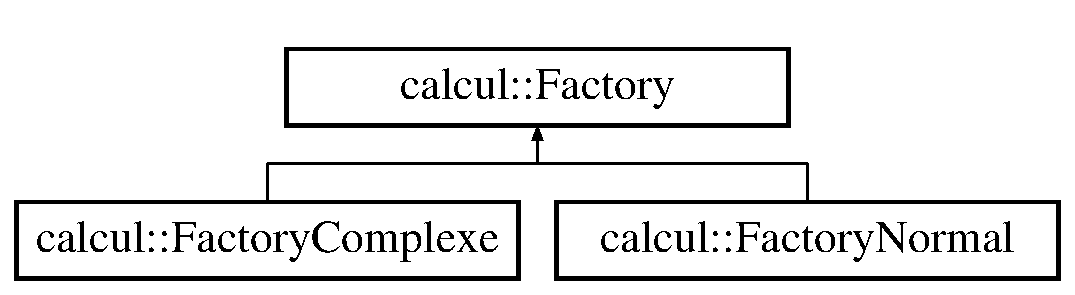
\includegraphics[height=2.000000cm]{classcalcul_1_1_factory}
\end{center}
\end{figure}
\subsection*{Fonctions membres publiques}
\begin{DoxyCompactItemize}
\item 
\hypertarget{classcalcul_1_1_factory_a359dd99c76b415398b59e757db6460ef}{virtual \hyperlink{classcalcul_1_1_cst}{Cst} \& {\bfseries Creer\-Reel} (Q\-String str)=0}\label{classcalcul_1_1_factory_a359dd99c76b415398b59e757db6460ef}

\item 
\hypertarget{classcalcul_1_1_factory_aa63c4d76b2435c896d83630f28f7ad20}{virtual \hyperlink{classcalcul_1_1_cst}{Cst} \& {\bfseries Creer\-Rationnel} (Q\-String str)=0}\label{classcalcul_1_1_factory_aa63c4d76b2435c896d83630f28f7ad20}

\item 
\hypertarget{classcalcul_1_1_factory_aa58cc259626e09447f944f020a21b01d}{virtual \hyperlink{classcalcul_1_1_cst}{Cst} \& {\bfseries Creer\-Entier} (Q\-String str)=0}\label{classcalcul_1_1_factory_aa58cc259626e09447f944f020a21b01d}

\end{DoxyCompactItemize}


\subsection{Description détaillée}
Classe abstraite implémentée en Design Pattern \hyperlink{classcalcul_1_1_factory}{Factory} Method pour créer des constantes. 

La documentation de cette classe a été générée à partir du fichier suivant \-:\begin{DoxyCompactItemize}
\item 
C\-:/\-Users/\-William/\-Dropbox/lo21/projet/\-Projet/factory.\-h\end{DoxyCompactItemize}

\hypertarget{classcalcul_1_1_factory_complexe}{\section{Référence de la classe calcul\-:\-:Factory\-Complexe}
\label{classcalcul_1_1_factory_complexe}\index{calcul\-::\-Factory\-Complexe@{calcul\-::\-Factory\-Complexe}}
}


Classe implémentée en Design Pattern \hyperlink{classcalcul_1_1_factory}{Factory} Method pour créer des constantes en mode complexe.  




{\ttfamily \#include $<$factory.\-h$>$}

Graphe d'héritage de calcul\-:\-:Factory\-Complexe\-:\begin{figure}[H]
\begin{center}
\leavevmode
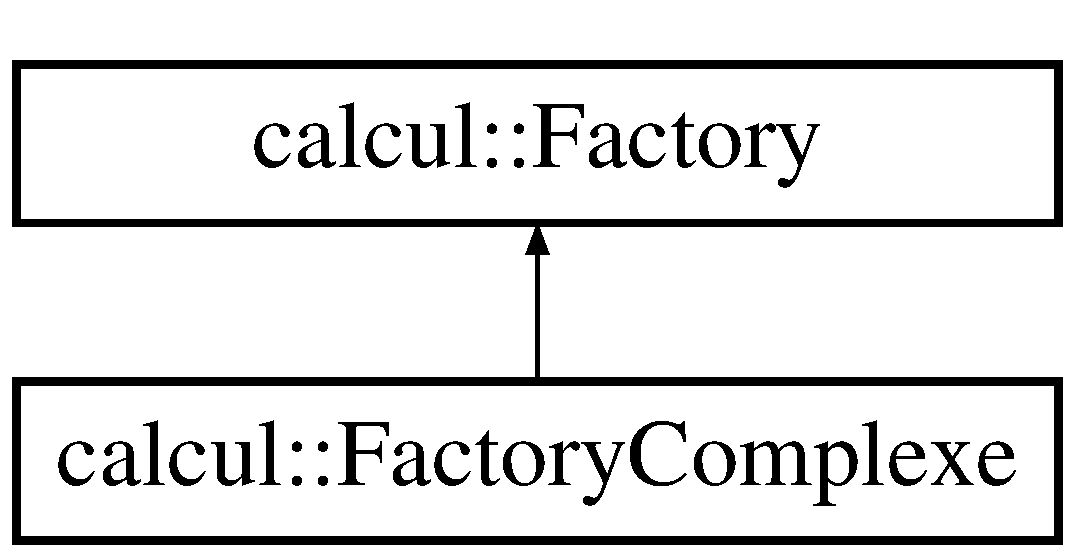
\includegraphics[height=2.000000cm]{classcalcul_1_1_factory_complexe}
\end{center}
\end{figure}
\subsection*{Fonctions membres publiques}
\begin{DoxyCompactItemize}
\item 
\hyperlink{classcalcul_1_1_complexe}{Complexe}$<$ \hyperlink{classcalcul_1_1_reel}{Reel} $>$ \& \hyperlink{classcalcul_1_1_factory_complexe_a0b9ebb21e377742ccdd9a5e2dff08b75}{Creer\-Reel} (Q\-String str)
\begin{DoxyCompactList}\small\item\em Créer une constante complexe réelle à partir d'une cha?ne de caractère passée en paramètre. \end{DoxyCompactList}\item 
\hyperlink{classcalcul_1_1_complexe}{Complexe}$<$ \hyperlink{classcalcul_1_1_rationnel}{Rationnel} $>$ \& \hyperlink{classcalcul_1_1_factory_complexe_abbbaea83b424942d01505936c1c9e5b2}{Creer\-Rationnel} (Q\-String str)
\begin{DoxyCompactList}\small\item\em Créer une constante complexe rationnelle à partir d'une cha?ne de caractère passée en paramètre. \end{DoxyCompactList}\item 
\hyperlink{classcalcul_1_1_complexe}{Complexe}$<$ \hyperlink{classcalcul_1_1_entier}{Entier} $>$ \& \hyperlink{classcalcul_1_1_factory_complexe_ab895838ce6abdae50203bdfd491dbe9c}{Creer\-Entier} (Q\-String str)
\begin{DoxyCompactList}\small\item\em Créer une constante complexe entière à partir d'une cha?ne de caractère passée en paramètre. \end{DoxyCompactList}\end{DoxyCompactItemize}


\subsection{Description détaillée}
Classe implémentée en Design Pattern \hyperlink{classcalcul_1_1_factory}{Factory} Method pour créer des constantes en mode complexe. 

\subsection{Documentation des fonctions membres}
\hypertarget{classcalcul_1_1_factory_complexe_ab895838ce6abdae50203bdfd491dbe9c}{\index{calcul\-::\-Factory\-Complexe@{calcul\-::\-Factory\-Complexe}!Creer\-Entier@{Creer\-Entier}}
\index{Creer\-Entier@{Creer\-Entier}!calcul::FactoryComplexe@{calcul\-::\-Factory\-Complexe}}
\subsubsection[{Creer\-Entier}]{\setlength{\rightskip}{0pt plus 5cm}{\bf Complexe}$<$ {\bf Entier} $>$ \& Factory\-Complexe\-::\-Creer\-Entier (
\begin{DoxyParamCaption}
\item[{Q\-String}]{str}
\end{DoxyParamCaption}
)\hspace{0.3cm}{\ttfamily [virtual]}}}\label{classcalcul_1_1_factory_complexe_ab895838ce6abdae50203bdfd491dbe9c}


Créer une constante complexe entière à partir d'une cha?ne de caractère passée en paramètre. 


\begin{DoxyParams}{Paramètres}
{\em \-:} & str La cha?ne de caractère à convertir \\
\hline
\end{DoxyParams}


Implémente \hyperlink{classcalcul_1_1_factory}{calcul\-::\-Factory}.

\hypertarget{classcalcul_1_1_factory_complexe_abbbaea83b424942d01505936c1c9e5b2}{\index{calcul\-::\-Factory\-Complexe@{calcul\-::\-Factory\-Complexe}!Creer\-Rationnel@{Creer\-Rationnel}}
\index{Creer\-Rationnel@{Creer\-Rationnel}!calcul::FactoryComplexe@{calcul\-::\-Factory\-Complexe}}
\subsubsection[{Creer\-Rationnel}]{\setlength{\rightskip}{0pt plus 5cm}{\bf Complexe}$<$ {\bf Rationnel} $>$ \& Factory\-Complexe\-::\-Creer\-Rationnel (
\begin{DoxyParamCaption}
\item[{Q\-String}]{str}
\end{DoxyParamCaption}
)\hspace{0.3cm}{\ttfamily [virtual]}}}\label{classcalcul_1_1_factory_complexe_abbbaea83b424942d01505936c1c9e5b2}


Créer une constante complexe rationnelle à partir d'une cha?ne de caractère passée en paramètre. 


\begin{DoxyParams}{Paramètres}
{\em \-:} & str La cha?ne de caractère à convertir \\
\hline
\end{DoxyParams}


Implémente \hyperlink{classcalcul_1_1_factory}{calcul\-::\-Factory}.

\hypertarget{classcalcul_1_1_factory_complexe_a0b9ebb21e377742ccdd9a5e2dff08b75}{\index{calcul\-::\-Factory\-Complexe@{calcul\-::\-Factory\-Complexe}!Creer\-Reel@{Creer\-Reel}}
\index{Creer\-Reel@{Creer\-Reel}!calcul::FactoryComplexe@{calcul\-::\-Factory\-Complexe}}
\subsubsection[{Creer\-Reel}]{\setlength{\rightskip}{0pt plus 5cm}{\bf Complexe}$<$ {\bf Reel} $>$ \& Factory\-Complexe\-::\-Creer\-Reel (
\begin{DoxyParamCaption}
\item[{Q\-String}]{str}
\end{DoxyParamCaption}
)\hspace{0.3cm}{\ttfamily [virtual]}}}\label{classcalcul_1_1_factory_complexe_a0b9ebb21e377742ccdd9a5e2dff08b75}


Créer une constante complexe réelle à partir d'une cha?ne de caractère passée en paramètre. 


\begin{DoxyParams}{Paramètres}
{\em \-:} & str La cha?ne de caractère à convertir \\
\hline
\end{DoxyParams}


Implémente \hyperlink{classcalcul_1_1_factory}{calcul\-::\-Factory}.



La documentation de cette classe a été générée à partir des fichiers suivants \-:\begin{DoxyCompactItemize}
\item 
C\-:/\-Users/\-William/\-Dropbox/lo21/projet/\-Projet/factory.\-h\item 
C\-:/\-Users/\-William/\-Dropbox/lo21/projet/\-Projet/factory.\-cpp\end{DoxyCompactItemize}

\hypertarget{class_factory_exception}{\section{Référence de la classe Factory\-Exception}
\label{class_factory_exception}\index{Factory\-Exception@{Factory\-Exception}}
}


On privilégie ses fils ce qui permet d'utiliser des traitements catch differents en fonction du type de l'erreur.  




{\ttfamily \#include $<$exception\-\_\-log.\-h$>$}

Graphe d'héritage de Factory\-Exception\-:\begin{figure}[H]
\begin{center}
\leavevmode
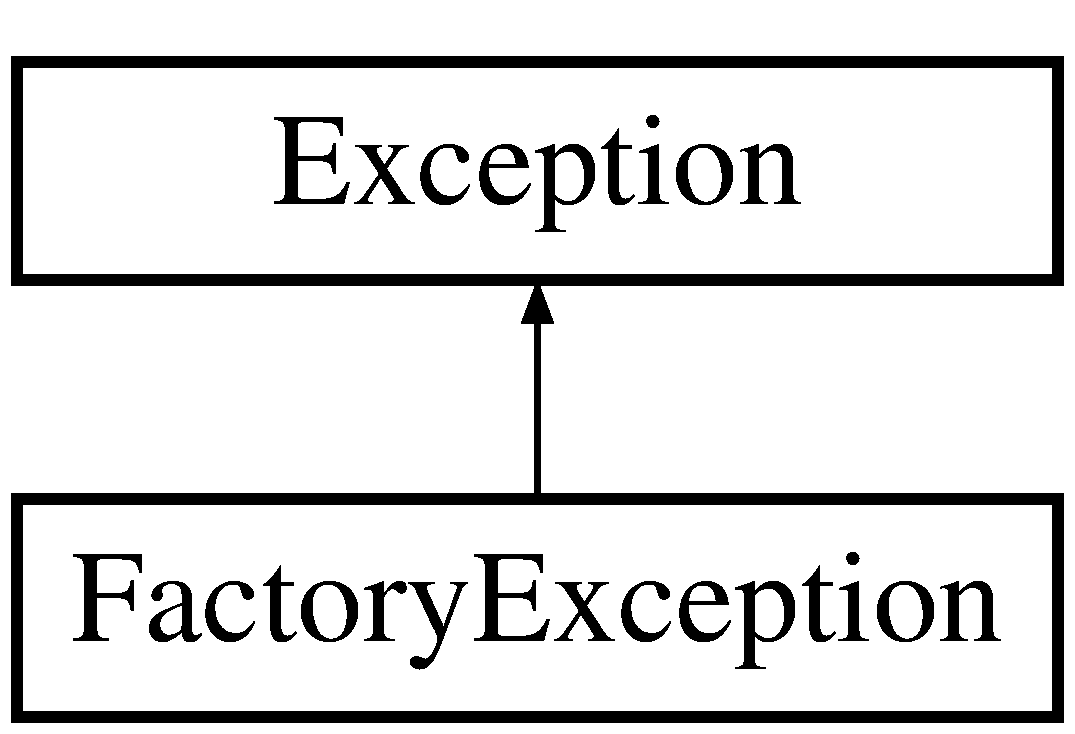
\includegraphics[height=2.000000cm]{class_factory_exception}
\end{center}
\end{figure}
\subsection*{Fonctions membres publiques}
\begin{DoxyCompactItemize}
\item 
\hyperlink{class_factory_exception_a4cfa20edeb011619ff2e42444a0e8de8}{Factory\-Exception} (Q\-String message)
\begin{DoxyCompactList}\small\item\em Constructeur de la classe \hyperlink{class_factory_exception}{Factory\-Exception}. \end{DoxyCompactList}\item 
\hypertarget{class_factory_exception_ab83319a32911e541798a6b01693c3839}{const \hyperlink{class_exception}{Exception} \& \hyperlink{class_factory_exception_ab83319a32911e541798a6b01693c3839}{send\-Message} () const }\label{class_factory_exception_ab83319a32911e541798a6b01693c3839}

\begin{DoxyCompactList}\small\item\em Méthode qui crée une boîte de diaglogue pour l'exception. \end{DoxyCompactList}\item 
\hypertarget{class_factory_exception_aa295318bdcc5145a99fefe7a4aa3639e}{const \hyperlink{class_exception}{Exception} \& \hyperlink{class_factory_exception_aa295318bdcc5145a99fefe7a4aa3639e}{send\-Log} () const }\label{class_factory_exception_aa295318bdcc5145a99fefe7a4aa3639e}

\begin{DoxyCompactList}\small\item\em Méthode qui envoie le message d'exception au Logsysteme. \end{DoxyCompactList}\end{DoxyCompactItemize}
\subsection*{Additional Inherited Members}


\subsection{Description détaillée}
On privilégie ses fils ce qui permet d'utiliser des traitements catch differents en fonction du type de l'erreur. 

\subsection{Documentation des constructeurs et destructeur}
\hypertarget{class_factory_exception_a4cfa20edeb011619ff2e42444a0e8de8}{\index{Factory\-Exception@{Factory\-Exception}!Factory\-Exception@{Factory\-Exception}}
\index{Factory\-Exception@{Factory\-Exception}!FactoryException@{Factory\-Exception}}
\subsubsection[{Factory\-Exception}]{\setlength{\rightskip}{0pt plus 5cm}Factory\-Exception\-::\-Factory\-Exception (
\begin{DoxyParamCaption}
\item[{Q\-String}]{message}
\end{DoxyParamCaption}
)\hspace{0.3cm}{\ttfamily [inline]}}}\label{class_factory_exception_a4cfa20edeb011619ff2e42444a0e8de8}


Constructeur de la classe \hyperlink{class_factory_exception}{Factory\-Exception}. 


\begin{DoxyParams}{Paramètres}
{\em message} & \-: Le message de l'exception \\
\hline
\end{DoxyParams}


La documentation de cette classe a été générée à partir du fichier suivant \-:\begin{DoxyCompactItemize}
\item 
C\-:/\-Users/\-William/\-Dropbox/lo21/projet/\-Projet/exception\-\_\-log.\-h\end{DoxyCompactItemize}

\hypertarget{classcalcul_1_1_factory_normal}{\section{Référence de la classe calcul\-:\-:Factory\-Normal}
\label{classcalcul_1_1_factory_normal}\index{calcul\-::\-Factory\-Normal@{calcul\-::\-Factory\-Normal}}
}


Classe implémentée en Design Pattern \hyperlink{classcalcul_1_1_factory}{Factory} Method pour créer des constantes en mode non-\/complexe.  




{\ttfamily \#include $<$factory.\-h$>$}

Graphe d'héritage de calcul\-:\-:Factory\-Normal\-:\begin{figure}[H]
\begin{center}
\leavevmode
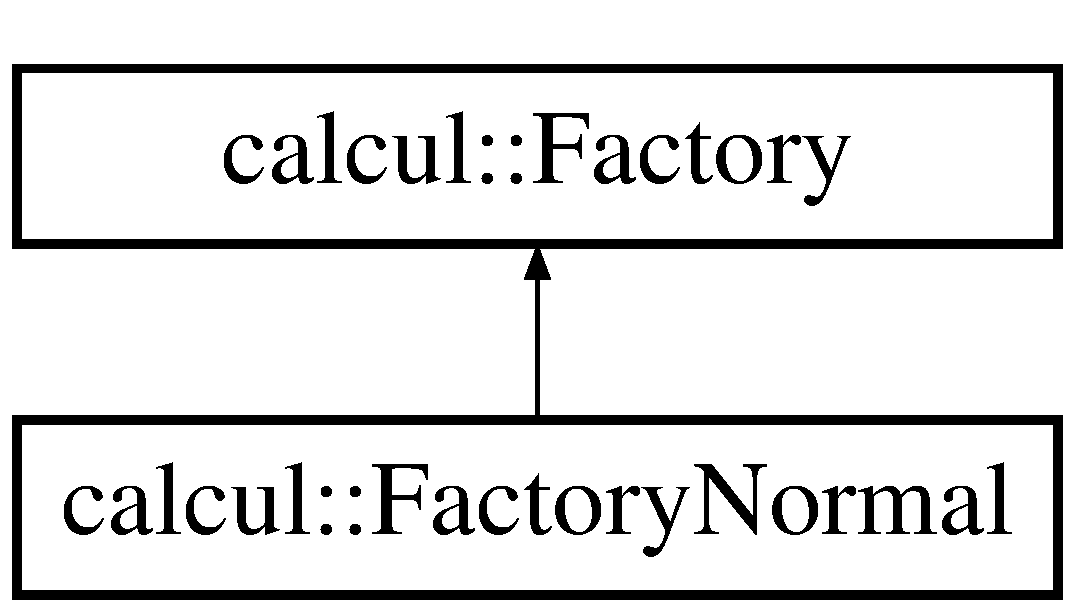
\includegraphics[height=2.000000cm]{classcalcul_1_1_factory_normal}
\end{center}
\end{figure}
\subsection*{Fonctions membres publiques}
\begin{DoxyCompactItemize}
\item 
\hyperlink{classcalcul_1_1_reel}{Reel} \& \hyperlink{classcalcul_1_1_factory_normal_a384ce0e05a619761d91ba08bd48729a1}{Creer\-Reel} (Q\-String str)
\begin{DoxyCompactList}\small\item\em Créer une constante réelle à partir d'une cha?ne de caractère passée en paramètre. \end{DoxyCompactList}\item 
\hyperlink{classcalcul_1_1_rationnel}{Rationnel} \& \hyperlink{classcalcul_1_1_factory_normal_a097039535ac042f0e15d0cd2473eb6f2}{Creer\-Rationnel} (Q\-String str)
\begin{DoxyCompactList}\small\item\em Créer une constante rationnelle à partir d'une cha?ne de caractère passée en paramètre. \end{DoxyCompactList}\item 
\hyperlink{classcalcul_1_1_entier}{Entier} \& \hyperlink{classcalcul_1_1_factory_normal_aa5214b571ca6e95c2fc61afd7a761680}{Creer\-Entier} (Q\-String str)
\begin{DoxyCompactList}\small\item\em Créer une constante entière à partir d'une cha?ne de caractère passée en paramètre. \end{DoxyCompactList}\end{DoxyCompactItemize}


\subsection{Description détaillée}
Classe implémentée en Design Pattern \hyperlink{classcalcul_1_1_factory}{Factory} Method pour créer des constantes en mode non-\/complexe. 

\subsection{Documentation des fonctions membres}
\hypertarget{classcalcul_1_1_factory_normal_aa5214b571ca6e95c2fc61afd7a761680}{\index{calcul\-::\-Factory\-Normal@{calcul\-::\-Factory\-Normal}!Creer\-Entier@{Creer\-Entier}}
\index{Creer\-Entier@{Creer\-Entier}!calcul::FactoryNormal@{calcul\-::\-Factory\-Normal}}
\subsubsection[{Creer\-Entier}]{\setlength{\rightskip}{0pt plus 5cm}{\bf Entier} \& Factory\-Normal\-::\-Creer\-Entier (
\begin{DoxyParamCaption}
\item[{Q\-String}]{str}
\end{DoxyParamCaption}
)\hspace{0.3cm}{\ttfamily [virtual]}}}\label{classcalcul_1_1_factory_normal_aa5214b571ca6e95c2fc61afd7a761680}


Créer une constante entière à partir d'une cha?ne de caractère passée en paramètre. 


\begin{DoxyParams}{Paramètres}
{\em \-:} & str La cha?ne de caractère à convertir \\
\hline
\end{DoxyParams}


Implémente \hyperlink{classcalcul_1_1_factory}{calcul\-::\-Factory}.

\hypertarget{classcalcul_1_1_factory_normal_a097039535ac042f0e15d0cd2473eb6f2}{\index{calcul\-::\-Factory\-Normal@{calcul\-::\-Factory\-Normal}!Creer\-Rationnel@{Creer\-Rationnel}}
\index{Creer\-Rationnel@{Creer\-Rationnel}!calcul::FactoryNormal@{calcul\-::\-Factory\-Normal}}
\subsubsection[{Creer\-Rationnel}]{\setlength{\rightskip}{0pt plus 5cm}{\bf Rationnel} \& Factory\-Normal\-::\-Creer\-Rationnel (
\begin{DoxyParamCaption}
\item[{Q\-String}]{str}
\end{DoxyParamCaption}
)\hspace{0.3cm}{\ttfamily [virtual]}}}\label{classcalcul_1_1_factory_normal_a097039535ac042f0e15d0cd2473eb6f2}


Créer une constante rationnelle à partir d'une cha?ne de caractère passée en paramètre. 


\begin{DoxyParams}{Paramètres}
{\em \-:} & str La cha?ne de caractère à convertir \\
\hline
\end{DoxyParams}


Implémente \hyperlink{classcalcul_1_1_factory}{calcul\-::\-Factory}.

\hypertarget{classcalcul_1_1_factory_normal_a384ce0e05a619761d91ba08bd48729a1}{\index{calcul\-::\-Factory\-Normal@{calcul\-::\-Factory\-Normal}!Creer\-Reel@{Creer\-Reel}}
\index{Creer\-Reel@{Creer\-Reel}!calcul::FactoryNormal@{calcul\-::\-Factory\-Normal}}
\subsubsection[{Creer\-Reel}]{\setlength{\rightskip}{0pt plus 5cm}{\bf Reel} \& Factory\-Normal\-::\-Creer\-Reel (
\begin{DoxyParamCaption}
\item[{Q\-String}]{str}
\end{DoxyParamCaption}
)\hspace{0.3cm}{\ttfamily [virtual]}}}\label{classcalcul_1_1_factory_normal_a384ce0e05a619761d91ba08bd48729a1}


Créer une constante réelle à partir d'une cha?ne de caractère passée en paramètre. 


\begin{DoxyParams}{Paramètres}
{\em \-:} & str La cha?ne de caractère à convertir \\
\hline
\end{DoxyParams}


Implémente \hyperlink{classcalcul_1_1_factory}{calcul\-::\-Factory}.



La documentation de cette classe a été générée à partir des fichiers suivants \-:\begin{DoxyCompactItemize}
\item 
C\-:/\-Users/\-William/\-Dropbox/lo21/projet/\-Projet/factory.\-h\item 
C\-:/\-Users/\-William/\-Dropbox/lo21/projet/\-Projet/factory.\-cpp\end{DoxyCompactItemize}

\hypertarget{class_log_systeme_1_1_log_message}{\section{Référence de la classe Log\-Systeme\-:\-:Log\-Message}
\label{class_log_systeme_1_1_log_message}\index{Log\-Systeme\-::\-Log\-Message@{Log\-Systeme\-::\-Log\-Message}}
}


La classe \hyperlink{class_log_systeme_1_1_log_message}{Log\-Message} est une classe ephemere qui n'a pour seul but que de diffuser son message sur les flux voulu.  




{\ttfamily \#include $<$exception\-\_\-log.\-h$>$}

\subsection*{Fonctions membres publiques}
\begin{DoxyCompactItemize}
\item 
\hyperlink{class_log_systeme_1_1_log_message_a0471a9f3e5824be53ba38a7bab8a4dd6}{Log\-Message} (Q\-String message, int priorite)
\begin{DoxyCompactList}\small\item\em Constructeur de la classe \hyperlink{class_log_systeme_1_1_log_message}{Log\-Message}. \end{DoxyCompactList}\item 
\hypertarget{class_log_systeme_1_1_log_message_a75f3cd2c8d73b2584790a8db3aa31574}{void \hyperlink{class_log_systeme_1_1_log_message_a75f3cd2c8d73b2584790a8db3aa31574}{add\-Fichier} ()}\label{class_log_systeme_1_1_log_message_a75f3cd2c8d73b2584790a8db3aa31574}

\begin{DoxyCompactList}\small\item\em Créer un fichier pour le log. \end{DoxyCompactList}\end{DoxyCompactItemize}


\subsection{Description détaillée}
La classe \hyperlink{class_log_systeme_1_1_log_message}{Log\-Message} est une classe ephemere qui n'a pour seul but que de diffuser son message sur les flux voulu. 

\subsection{Documentation des constructeurs et destructeur}
\hypertarget{class_log_systeme_1_1_log_message_a0471a9f3e5824be53ba38a7bab8a4dd6}{\index{Log\-Systeme\-::\-Log\-Message@{Log\-Systeme\-::\-Log\-Message}!Log\-Message@{Log\-Message}}
\index{Log\-Message@{Log\-Message}!LogSysteme::LogMessage@{Log\-Systeme\-::\-Log\-Message}}
\subsubsection[{Log\-Message}]{\setlength{\rightskip}{0pt plus 5cm}Log\-Systeme\-::\-Log\-Message\-::\-Log\-Message (
\begin{DoxyParamCaption}
\item[{Q\-String}]{message, }
\item[{int}]{priorite}
\end{DoxyParamCaption}
)\hspace{0.3cm}{\ttfamily [inline]}}}\label{class_log_systeme_1_1_log_message_a0471a9f3e5824be53ba38a7bab8a4dd6}


Constructeur de la classe \hyperlink{class_log_systeme_1_1_log_message}{Log\-Message}. 


\begin{DoxyParams}{Paramètres}
{\em message} & \-: Le message à ajouter dans le log \\
\hline
{\em priorite} & \-: La priorité du message \\
\hline
\end{DoxyParams}


La documentation de cette classe a été générée à partir des fichiers suivants \-:\begin{DoxyCompactItemize}
\item 
C\-:/\-Users/\-William/\-Dropbox/lo21/projet/\-Projet/exception\-\_\-log.\-h\item 
C\-:/\-Users/\-William/\-Dropbox/lo21/projet/\-Projet/exception\-\_\-log.\-cpp\end{DoxyCompactItemize}

\hypertarget{class_log_systeme}{\section{Référence de la classe Log\-Systeme}
\label{class_log_systeme}\index{Log\-Systeme@{Log\-Systeme}}
}


La classe \hyperlink{class_log_systeme}{Log\-Systeme} est la classe charge de gere des logs messages. Elle est implémentée en Design pattern singleton. Elle re?oit une demande d'ajout de log venant du programme et crée ainsi une instance log message qu'elle supprime apres qu'elle aie envoyé son message sur la console et dans le fichier.  




{\ttfamily \#include $<$exception\-\_\-log.\-h$>$}

\subsection*{Classes}
\begin{DoxyCompactItemize}
\item 
class \hyperlink{class_log_systeme_1_1_log_message}{Log\-Message}
\begin{DoxyCompactList}\small\item\em La classe \hyperlink{class_log_systeme_1_1_log_message}{Log\-Message} est une classe ephemere qui n'a pour seul but que de diffuser son message sur les flux voulu. \end{DoxyCompactList}\end{DoxyCompactItemize}
\subsection*{Fonctions membres publiques}
\begin{DoxyCompactItemize}
\item 
void \hyperlink{class_log_systeme_a0b550ea4cee3de636dccdfd253f1f82e}{add\-Log} (Q\-String str, int priorite)
\begin{DoxyCompactList}\small\item\em Ajouter un message dans le log. \end{DoxyCompactList}\end{DoxyCompactItemize}
\subsection*{Fonctions membres publiques statiques}
\begin{DoxyCompactItemize}
\item 
\hypertarget{class_log_systeme_a6d3fb70725266f36fe575a904bc03c5f}{static \hyperlink{class_log_systeme}{Log\-Systeme} \& \hyperlink{class_log_systeme_a6d3fb70725266f36fe575a904bc03c5f}{get\-Instance\-Log} ()}\label{class_log_systeme_a6d3fb70725266f36fe575a904bc03c5f}

\begin{DoxyCompactList}\small\item\em Récupérer l'instance du \hyperlink{class_log_systeme}{Log\-Systeme}. \end{DoxyCompactList}\item 
\hypertarget{class_log_systeme_a746b4b013f9a5efeda1934da779fadc4}{static void \hyperlink{class_log_systeme_a746b4b013f9a5efeda1934da779fadc4}{libere\-Instance} ()}\label{class_log_systeme_a746b4b013f9a5efeda1934da779fadc4}

\begin{DoxyCompactList}\small\item\em Libérer l'instance du \hyperlink{class_log_systeme}{Log\-Systeme}. \end{DoxyCompactList}\end{DoxyCompactItemize}


\subsection{Description détaillée}
La classe \hyperlink{class_log_systeme}{Log\-Systeme} est la classe charge de gere des logs messages. Elle est implémentée en Design pattern singleton. Elle re?oit une demande d'ajout de log venant du programme et crée ainsi une instance log message qu'elle supprime apres qu'elle aie envoyé son message sur la console et dans le fichier. 

\subsection{Documentation des fonctions membres}
\hypertarget{class_log_systeme_a0b550ea4cee3de636dccdfd253f1f82e}{\index{Log\-Systeme@{Log\-Systeme}!add\-Log@{add\-Log}}
\index{add\-Log@{add\-Log}!LogSysteme@{Log\-Systeme}}
\subsubsection[{add\-Log}]{\setlength{\rightskip}{0pt plus 5cm}void Log\-Systeme\-::add\-Log (
\begin{DoxyParamCaption}
\item[{Q\-String}]{str, }
\item[{int}]{priorite}
\end{DoxyParamCaption}
)}}\label{class_log_systeme_a0b550ea4cee3de636dccdfd253f1f82e}


Ajouter un message dans le log. 


\begin{DoxyParams}{Paramètres}
{\em \-:} & str Le message à écrire dans le log \\
\hline
{\em \-:} & priorite La priorit?? du message \\
\hline
\end{DoxyParams}


La documentation de cette classe a été générée à partir des fichiers suivants \-:\begin{DoxyCompactItemize}
\item 
C\-:/\-Users/\-William/\-Dropbox/lo21/projet/\-Projet/exception\-\_\-log.\-h\item 
C\-:/\-Users/\-William/\-Dropbox/lo21/projet/\-Projet/exception\-\_\-log.\-cpp\end{DoxyCompactItemize}

\hypertarget{classcalcul_1_1_moteur_calcul}{\section{Référence de la classe calcul\-:\-:Moteur\-Calcul}
\label{classcalcul_1_1_moteur_calcul}\index{calcul\-::\-Moteur\-Calcul@{calcul\-::\-Moteur\-Calcul}}
}


Classe representant le moteur de calcul.  




{\ttfamily \#include $<$moteur\-Calcul.\-h$>$}

\subsection*{Fonctions membres publiques}
\begin{DoxyCompactItemize}
\item 
\hypertarget{classcalcul_1_1_moteur_calcul_abc502459962881c55c52273d0445eb27}{\hyperlink{classcalcul_1_1_moteur_calcul_abc502459962881c55c52273d0445eb27}{Moteur\-Calcul} ()}\label{classcalcul_1_1_moteur_calcul_abc502459962881c55c52273d0445eb27}

\begin{DoxyCompactList}\small\item\em Constructeur par défaut du moteur de calcul. \end{DoxyCompactList}\item 
\hyperlink{classcalcul_1_1_moteur_calcul_a08099d4c72376d5bef0aa14c43f08733}{Moteur\-Calcul} (\hyperlink{classcalcul_1_1_moteur_calcul}{Moteur\-Calcul} \&a\-\_\-copier)
\begin{DoxyCompactList}\small\item\em Constructeur de recopie du moteur de calcul. \end{DoxyCompactList}\item 
void \hyperlink{classcalcul_1_1_moteur_calcul_af0433c3b84f5aae984fc94feef12ce4e}{ajouter\-Resoudre} (Q\-String ajout)
\begin{DoxyCompactList}\small\item\em Ajouter dans la pile de stockage une cha?ne de caractère passée en paramètre et résoud l'expression si le dernier élément est un opérateur. \end{DoxyCompactList}\item 
const \hyperlink{classcalcul_1_1_pile_cst}{Pile\-Cst} \& \hyperlink{classcalcul_1_1_moteur_calcul_a7283f0b19699bccf7062d3c791832ffa}{get\-Pile} () const 
\begin{DoxyCompactList}\small\item\em Récupérer la pile de constantes. \end{DoxyCompactList}\item 
void \hyperlink{classcalcul_1_1_moteur_calcul_a8e4aae58c5cb9102cb724a90c52563d9}{changer\-Mode} (Q\-String mode\-\_\-type=\char`\"{}C\char`\"{})
\begin{DoxyCompactList}\small\item\em Changer le mode de calcul. \end{DoxyCompactList}\item 
void \hyperlink{classcalcul_1_1_moteur_calcul_acbd9ee3b5e3b7b3004131bd4a2e4576e}{changer\-Angle} (Q\-String mode\-\_\-angle=\char`\"{}degre\char`\"{})
\begin{DoxyCompactList}\small\item\em Changer le mode d'angle. \end{DoxyCompactList}\end{DoxyCompactItemize}


\subsection{Description détaillée}
Classe representant le moteur de calcul. 

\subsection{Documentation des constructeurs et destructeur}
\hypertarget{classcalcul_1_1_moteur_calcul_a08099d4c72376d5bef0aa14c43f08733}{\index{calcul\-::\-Moteur\-Calcul@{calcul\-::\-Moteur\-Calcul}!Moteur\-Calcul@{Moteur\-Calcul}}
\index{Moteur\-Calcul@{Moteur\-Calcul}!calcul::MoteurCalcul@{calcul\-::\-Moteur\-Calcul}}
\subsubsection[{Moteur\-Calcul}]{\setlength{\rightskip}{0pt plus 5cm}calcul\-::\-Moteur\-Calcul\-::\-Moteur\-Calcul (
\begin{DoxyParamCaption}
\item[{{\bf Moteur\-Calcul} \&}]{a\-\_\-copier}
\end{DoxyParamCaption}
)\hspace{0.3cm}{\ttfamily [inline]}}}\label{classcalcul_1_1_moteur_calcul_a08099d4c72376d5bef0aa14c43f08733}


Constructeur de recopie du moteur de calcul. 


\begin{DoxyParams}{Paramètres}
{\em a\-\_\-copier} & \-: a\-\_\-copier Une référence de moteur de calcul à recopier \\
\hline
\end{DoxyParams}


\subsection{Documentation des fonctions membres}
\hypertarget{classcalcul_1_1_moteur_calcul_af0433c3b84f5aae984fc94feef12ce4e}{\index{calcul\-::\-Moteur\-Calcul@{calcul\-::\-Moteur\-Calcul}!ajouter\-Resoudre@{ajouter\-Resoudre}}
\index{ajouter\-Resoudre@{ajouter\-Resoudre}!calcul::MoteurCalcul@{calcul\-::\-Moteur\-Calcul}}
\subsubsection[{ajouter\-Resoudre}]{\setlength{\rightskip}{0pt plus 5cm}void Moteur\-Calcul\-::ajouter\-Resoudre (
\begin{DoxyParamCaption}
\item[{Q\-String}]{ajout}
\end{DoxyParamCaption}
)}}\label{classcalcul_1_1_moteur_calcul_af0433c3b84f5aae984fc94feef12ce4e}


Ajouter dans la pile de stockage une cha?ne de caractère passée en paramètre et résoud l'expression si le dernier élément est un opérateur. 


\begin{DoxyParams}{Paramètres}
{\em ajout} & \-: La cha?ne de caractère à ajouter dans la pile de stockage \\
\hline
\end{DoxyParams}
\hypertarget{classcalcul_1_1_moteur_calcul_acbd9ee3b5e3b7b3004131bd4a2e4576e}{\index{calcul\-::\-Moteur\-Calcul@{calcul\-::\-Moteur\-Calcul}!changer\-Angle@{changer\-Angle}}
\index{changer\-Angle@{changer\-Angle}!calcul::MoteurCalcul@{calcul\-::\-Moteur\-Calcul}}
\subsubsection[{changer\-Angle}]{\setlength{\rightskip}{0pt plus 5cm}void Moteur\-Calcul\-::changer\-Angle (
\begin{DoxyParamCaption}
\item[{Q\-String}]{mode\-\_\-angle = {\ttfamily \char`\"{}degre\char`\"{}}}
\end{DoxyParamCaption}
)}}\label{classcalcul_1_1_moteur_calcul_acbd9ee3b5e3b7b3004131bd4a2e4576e}


Changer le mode d'angle. 


\begin{DoxyParams}{Paramètres}
{\em mode\-\_\-angle} & \-: Le nouveau mode d'angle \\
\hline
\end{DoxyParams}
\hypertarget{classcalcul_1_1_moteur_calcul_a8e4aae58c5cb9102cb724a90c52563d9}{\index{calcul\-::\-Moteur\-Calcul@{calcul\-::\-Moteur\-Calcul}!changer\-Mode@{changer\-Mode}}
\index{changer\-Mode@{changer\-Mode}!calcul::MoteurCalcul@{calcul\-::\-Moteur\-Calcul}}
\subsubsection[{changer\-Mode}]{\setlength{\rightskip}{0pt plus 5cm}void Moteur\-Calcul\-::changer\-Mode (
\begin{DoxyParamCaption}
\item[{Q\-String}]{mode\-\_\-type = {\ttfamily \char`\"{}C\char`\"{}}}
\end{DoxyParamCaption}
)}}\label{classcalcul_1_1_moteur_calcul_a8e4aae58c5cb9102cb724a90c52563d9}


Changer le mode de calcul. 


\begin{DoxyParams}{Paramètres}
{\em mode\-\_\-type} & \-: Le nouveau mode de calcul \\
\hline
\end{DoxyParams}
\hypertarget{classcalcul_1_1_moteur_calcul_a7283f0b19699bccf7062d3c791832ffa}{\index{calcul\-::\-Moteur\-Calcul@{calcul\-::\-Moteur\-Calcul}!get\-Pile@{get\-Pile}}
\index{get\-Pile@{get\-Pile}!calcul::MoteurCalcul@{calcul\-::\-Moteur\-Calcul}}
\subsubsection[{get\-Pile}]{\setlength{\rightskip}{0pt plus 5cm}const {\bf Pile\-Cst}\& calcul\-::\-Moteur\-Calcul\-::get\-Pile (
\begin{DoxyParamCaption}
{}
\end{DoxyParamCaption}
) const\hspace{0.3cm}{\ttfamily [inline]}}}\label{classcalcul_1_1_moteur_calcul_a7283f0b19699bccf7062d3c791832ffa}


Récupérer la pile de constantes. 

\begin{DoxyReturn}{Renvoie}
La pile de stockage 
\end{DoxyReturn}


La documentation de cette classe a été générée à partir des fichiers suivants \-:\begin{DoxyCompactItemize}
\item 
C\-:/\-Users/\-William/\-Dropbox/lo21/projet/\-Projet/moteur\-Calcul.\-h\item 
C\-:/\-Users/\-William/\-Dropbox/lo21/projet/\-Projet/moteur\-Calcul.\-cpp\end{DoxyCompactItemize}

\hypertarget{class_onglet}{\section{Référence de la classe Onglet}
\label{class_onglet}\index{Onglet@{Onglet}}
}


Classe representant l'onglet qui hérite d'un Q\-Widget.  




{\ttfamily \#include $<$onglet.\-h$>$}

\subsection*{Classes}
\begin{DoxyCompactItemize}
\item 
class \hyperlink{class_onglet_1_1evenement}{evenement}
\begin{DoxyCompactList}\small\item\em Classe interne pour traiter les évenements. \end{DoxyCompactList}\end{DoxyCompactItemize}
\subsection*{Connecteurs publics}
\begin{DoxyCompactItemize}
\item 
\hypertarget{class_onglet_a483593c077f1867feb1d79e86a70d1fd}{void \hyperlink{class_onglet_a483593c077f1867feb1d79e86a70d1fd}{traitement\-Mode} ()}\label{class_onglet_a483593c077f1867feb1d79e86a70d1fd}

\begin{DoxyCompactList}\small\item\em Change le mode de calcul et active les boutons correspondants quand l'utilisateur change de type de constantes, active ou déactive le mode complexe. \end{DoxyCompactList}\item 
\hypertarget{class_onglet_a08179a7a267b0f8a0cc18008b1385fae}{void \hyperlink{class_onglet_a08179a7a267b0f8a0cc18008b1385fae}{traitement\-Angle} ()}\label{class_onglet_a08179a7a267b0f8a0cc18008b1385fae}

\begin{DoxyCompactList}\small\item\em Change le mode d'angle. \end{DoxyCompactList}\item 
\hypertarget{class_onglet_ab77c8b306abc044025f1112e90c546f0}{void \hyperlink{class_onglet_ab77c8b306abc044025f1112e90c546f0}{traitement\-Boutons} ()}\label{class_onglet_ab77c8b306abc044025f1112e90c546f0}

\begin{DoxyCompactList}\small\item\em Agir selon le bouton appuyé \end{DoxyCompactList}\item 
\hypertarget{class_onglet_a6fa52eb0489ba767dc4ecf6776c6d8ff}{void \hyperlink{class_onglet_a6fa52eb0489ba767dc4ecf6776c6d8ff}{traitement\-Clavier} ()}\label{class_onglet_a6fa52eb0489ba767dc4ecf6776c6d8ff}

\begin{DoxyCompactList}\small\item\em Afficher ou cacher les clavier. \end{DoxyCompactList}\item 
\hypertarget{class_onglet_a6cf54809c9359f5b2b97b273fde77e05}{void \hyperlink{class_onglet_a6cf54809c9359f5b2b97b273fde77e05}{new\-Onglet} ()}\label{class_onglet_a6cf54809c9359f5b2b97b273fde77e05}

\begin{DoxyCompactList}\small\item\em Créer un nouvel onglet vide quand C\-T\-R\-L+\-N appuyé \end{DoxyCompactList}\item 
\hypertarget{class_onglet_a76074598b99789f3b17d2bf99418aeda}{void \hyperlink{class_onglet_a76074598b99789f3b17d2bf99418aeda}{delete\-Onglet} ()}\label{class_onglet_a76074598b99789f3b17d2bf99418aeda}

\begin{DoxyCompactList}\small\item\em Supprimer l'onglet actuel quand C\-T\-R\-L+\-W appuyé \end{DoxyCompactList}\item 
\hypertarget{class_onglet_a3f366c3138661e79f0656ed5eb668055}{void \hyperlink{class_onglet_a3f366c3138661e79f0656ed5eb668055}{dup\-Onglet} ()}\label{class_onglet_a3f366c3138661e79f0656ed5eb668055}

\begin{DoxyCompactList}\small\item\em Dupliquer l'onglet actuel quand C\-T\-R\-L+\-T appuyé \end{DoxyCompactList}\end{DoxyCompactItemize}
\subsection*{Fonctions membres publiques}
\begin{DoxyCompactItemize}
\item 
\hyperlink{class_onglet_a0d7cefa46e78a411930d9def60f4267f}{Onglet} (unsigned int num, Q\-Tab\-Widget $\ast$tab, bool init)
\begin{DoxyCompactList}\small\item\em Constructeur par défaut de la classe \hyperlink{class_onglet}{Onglet}. \end{DoxyCompactList}\item 
\hyperlink{class_onglet_aa5950fca5fadb7343c5e124b1c10f17c}{Onglet} (unsigned int num, Q\-Tab\-Widget $\ast$tab, \hyperlink{class_onglet}{Onglet} $\ast$o)
\begin{DoxyCompactList}\small\item\em Constructeur de recopie de la classe \hyperlink{class_onglet}{Onglet}. \end{DoxyCompactList}\item 
\hypertarget{class_onglet_a717d9bd0139081b4e779f552c835b0f5}{\hyperlink{class_onglet_a717d9bd0139081b4e779f552c835b0f5}{$\sim$\-Onglet} ()}\label{class_onglet_a717d9bd0139081b4e779f552c835b0f5}

\begin{DoxyCompactList}\small\item\em Destructeur de la classe \hyperlink{class_calculatrice}{Calculatrice}. \end{DoxyCompactList}\item 
\hyperlink{classcalcul_1_1_moteur_calcul}{Moteur\-Calcul} \hyperlink{class_onglet_ab534cdcfcdd5a02d0f872e1fcbc8df58}{get\-Mot} ()
\begin{DoxyCompactList}\small\item\em Retourner le moteur de calcul de l'onglet. \end{DoxyCompactList}\end{DoxyCompactItemize}


\subsection{Description détaillée}
Classe representant l'onglet qui hérite d'un Q\-Widget. 

\subsection{Documentation des constructeurs et destructeur}
\hypertarget{class_onglet_a0d7cefa46e78a411930d9def60f4267f}{\index{Onglet@{Onglet}!Onglet@{Onglet}}
\index{Onglet@{Onglet}!Onglet@{Onglet}}
\subsubsection[{Onglet}]{\setlength{\rightskip}{0pt plus 5cm}Onglet\-::\-Onglet (
\begin{DoxyParamCaption}
\item[{unsigned int}]{num, }
\item[{Q\-Tab\-Widget $\ast$}]{tab, }
\item[{bool}]{init}
\end{DoxyParamCaption}
)}}\label{class_onglet_a0d7cefa46e78a411930d9def60f4267f}


Constructeur par défaut de la classe \hyperlink{class_onglet}{Onglet}. 


\begin{DoxyParams}{Paramètres}
{\em num} & \-: Numéro de l'onglet \\
\hline
{\em tab} & \-: Pointeur du Q\-Tab\-Widget de la calculatrice pour stocker l'onglet \\
\hline
{\em init} & \-: true pour le premier onglet, false pour tout le reste \\
\hline
\end{DoxyParams}
\hypertarget{class_onglet_aa5950fca5fadb7343c5e124b1c10f17c}{\index{Onglet@{Onglet}!Onglet@{Onglet}}
\index{Onglet@{Onglet}!Onglet@{Onglet}}
\subsubsection[{Onglet}]{\setlength{\rightskip}{0pt plus 5cm}Onglet\-::\-Onglet (
\begin{DoxyParamCaption}
\item[{unsigned int}]{num, }
\item[{Q\-Tab\-Widget $\ast$}]{tab, }
\item[{{\bf Onglet} $\ast$}]{o}
\end{DoxyParamCaption}
)}}\label{class_onglet_aa5950fca5fadb7343c5e124b1c10f17c}


Constructeur de recopie de la classe \hyperlink{class_onglet}{Onglet}. 


\begin{DoxyParams}{Paramètres}
{\em num} & \-: Numéro de l'onglet \\
\hline
{\em tab} & \-: Pointeur du Q\-Tab\-Widget de la calculatrice pour stocker l'onglet \\
\hline
{\em o} & \-: Pointeur de l'onglet à dupliquer \\
\hline
\end{DoxyParams}


\subsection{Documentation des fonctions membres}
\hypertarget{class_onglet_ab534cdcfcdd5a02d0f872e1fcbc8df58}{\index{Onglet@{Onglet}!get\-Mot@{get\-Mot}}
\index{get\-Mot@{get\-Mot}!Onglet@{Onglet}}
\subsubsection[{get\-Mot}]{\setlength{\rightskip}{0pt plus 5cm}{\bf Moteur\-Calcul} Onglet\-::get\-Mot (
\begin{DoxyParamCaption}
{}
\end{DoxyParamCaption}
)\hspace{0.3cm}{\ttfamily [inline]}}}\label{class_onglet_ab534cdcfcdd5a02d0f872e1fcbc8df58}


Retourner le moteur de calcul de l'onglet. 

\begin{DoxyReturn}{Renvoie}
Le moteur de calcul 
\end{DoxyReturn}


La documentation de cette classe a été générée à partir des fichiers suivants \-:\begin{DoxyCompactItemize}
\item 
C\-:/\-Users/\-William/\-Dropbox/lo21/projet/\-Projet/onglet.\-h\item 
C\-:/\-Users/\-William/\-Dropbox/lo21/projet/\-Projet/onglet.\-cpp\end{DoxyCompactItemize}

\hypertarget{class_operation_exception}{\section{Référence de la classe Operation\-Exception}
\label{class_operation_exception}\index{Operation\-Exception@{Operation\-Exception}}
}


Hérite de la classe exception.  




{\ttfamily \#include $<$exception\-\_\-log.\-h$>$}

Graphe d'héritage de Operation\-Exception\-:\begin{figure}[H]
\begin{center}
\leavevmode
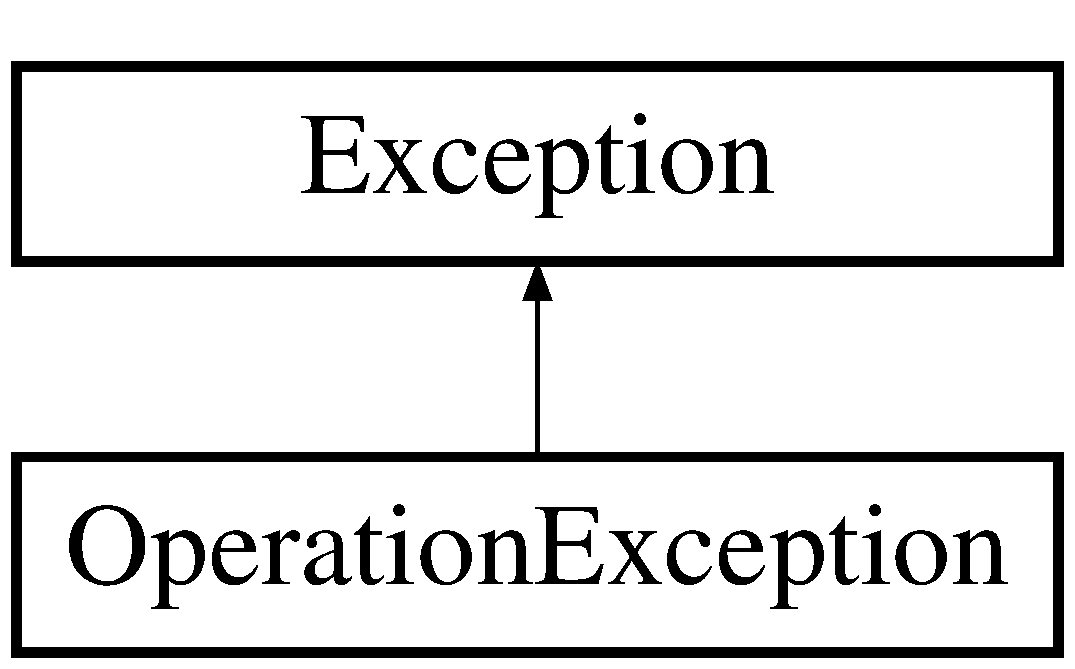
\includegraphics[height=2.000000cm]{class_operation_exception}
\end{center}
\end{figure}
\subsection*{Fonctions membres publiques}
\begin{DoxyCompactItemize}
\item 
\hyperlink{class_operation_exception_a4175f17d45ddeb69e496f46d10ee7715}{Operation\-Exception} (Q\-String message)
\begin{DoxyCompactList}\small\item\em Constructeur de la classe \hyperlink{class_operation_exception}{Operation\-Exception}. \end{DoxyCompactList}\item 
\hypertarget{class_operation_exception_ad0bc3c8efcd32fb7940c02cfbbe2f188}{const \hyperlink{class_exception}{Exception} \& \hyperlink{class_operation_exception_ad0bc3c8efcd32fb7940c02cfbbe2f188}{send\-Message} () const }\label{class_operation_exception_ad0bc3c8efcd32fb7940c02cfbbe2f188}

\begin{DoxyCompactList}\small\item\em Méthode qui crée une boîte de diaglogue pour l'exception. \end{DoxyCompactList}\item 
\hypertarget{class_operation_exception_aeef9c6fa3863aa3ab4c233077f090a65}{const \hyperlink{class_exception}{Exception} \& \hyperlink{class_operation_exception_aeef9c6fa3863aa3ab4c233077f090a65}{send\-Log} () const }\label{class_operation_exception_aeef9c6fa3863aa3ab4c233077f090a65}

\begin{DoxyCompactList}\small\item\em Méthode qui envoie le message d'exception au Logsysteme. \end{DoxyCompactList}\end{DoxyCompactItemize}
\subsection*{Additional Inherited Members}


\subsection{Description détaillée}
Hérite de la classe exception. 

\subsection{Documentation des constructeurs et destructeur}
\hypertarget{class_operation_exception_a4175f17d45ddeb69e496f46d10ee7715}{\index{Operation\-Exception@{Operation\-Exception}!Operation\-Exception@{Operation\-Exception}}
\index{Operation\-Exception@{Operation\-Exception}!OperationException@{Operation\-Exception}}
\subsubsection[{Operation\-Exception}]{\setlength{\rightskip}{0pt plus 5cm}Operation\-Exception\-::\-Operation\-Exception (
\begin{DoxyParamCaption}
\item[{Q\-String}]{message}
\end{DoxyParamCaption}
)\hspace{0.3cm}{\ttfamily [inline]}}}\label{class_operation_exception_a4175f17d45ddeb69e496f46d10ee7715}


Constructeur de la classe \hyperlink{class_operation_exception}{Operation\-Exception}. 


\begin{DoxyParams}{Paramètres}
{\em message} & \-: Le message de l'exception \\
\hline
\end{DoxyParams}


La documentation de cette classe a été générée à partir du fichier suivant \-:\begin{DoxyCompactItemize}
\item 
C\-:/\-Users/\-William/\-Dropbox/lo21/projet/\-Projet/exception\-\_\-log.\-h\end{DoxyCompactItemize}

\hypertarget{classcalcul_1_1_pile_cst}{\section{Référence de la classe calcul\-:\-:Pile\-Cst}
\label{classcalcul_1_1_pile_cst}\index{calcul\-::\-Pile\-Cst@{calcul\-::\-Pile\-Cst}}
}


Classe representant la pile de constantes.  




{\ttfamily \#include $<$pile\-Cst.\-h$>$}

\subsection*{Fonctions membres publiques}
\begin{DoxyCompactItemize}
\item 
\hypertarget{classcalcul_1_1_pile_cst_abf48d20785e9a7318d4cbe94a3270bd2}{\hyperlink{classcalcul_1_1_pile_cst_abf48d20785e9a7318d4cbe94a3270bd2}{Pile\-Cst} ()}\label{classcalcul_1_1_pile_cst_abf48d20785e9a7318d4cbe94a3270bd2}

\begin{DoxyCompactList}\small\item\em Constructeur par défaut de la pile de constantes. \end{DoxyCompactList}\item 
\hyperlink{classcalcul_1_1_pile_cst_aa4896a49196236731d6b7fe9fe33dcb2}{Pile\-Cst} (\hyperlink{classcalcul_1_1_pile_cst}{Pile\-Cst} \&a\-\_\-copier)
\begin{DoxyCompactList}\small\item\em Constructeur de recopie de la pile de constantes. \end{DoxyCompactList}\item 
\hypertarget{classcalcul_1_1_pile_cst_a5c08e241bc25523978e672099093816f}{\hyperlink{classcalcul_1_1_pile_cst_a5c08e241bc25523978e672099093816f}{$\sim$\-Pile\-Cst} ()}\label{classcalcul_1_1_pile_cst_a5c08e241bc25523978e672099093816f}

\begin{DoxyCompactList}\small\item\em Destructeur de la pile de constantes. \end{DoxyCompactList}\item 
void \hyperlink{classcalcul_1_1_pile_cst_a7b4bff3fb4025a773adb6eb5a76d7835}{set\-Mode} (Mode\-Type new\-\_\-mode)
\begin{DoxyCompactList}\small\item\em Configurer le mode de calcul de la pile. \end{DoxyCompactList}\item 
void \hyperlink{classcalcul_1_1_pile_cst_adff97011a52d468cdefbe34fce28bb14}{set\-Angle} (Angle\-Type new\-\_\-angle)
\begin{DoxyCompactList}\small\item\em Configurer le mode d'angle de la pile. \end{DoxyCompactList}\item 
Q\-String \hyperlink{classcalcul_1_1_pile_cst_a6db73772c41a3ec56683563cd5734a1f}{get\-String} () const 
\begin{DoxyCompactList}\small\item\em Récupérer la chaîne de caractères associée à la pile. \end{DoxyCompactList}\item 
const Q\-Stack$<$ \hyperlink{classcalcul_1_1_cst}{Cst} $\ast$ $>$ \& \hyperlink{classcalcul_1_1_pile_cst_a464aa7bf622f538756f39014686fcda8}{get\-Pile} () const 
\begin{DoxyCompactList}\small\item\em Récupérer la pile de constantes. \end{DoxyCompactList}\item 
bool \hyperlink{classcalcul_1_1_pile_cst_a1e0258011489a1887020d6f89d0f7726}{vide\-Cst} () const 
\begin{DoxyCompactList}\small\item\em Vérifier si la pile est vide. \end{DoxyCompactList}\item 
void \hyperlink{classcalcul_1_1_pile_cst_a5709199aa15152382a8fc27d6c54bfb2}{ajouter} (Q\-String str)
\begin{DoxyCompactList}\small\item\em Ajouter une chaîne de caractères à la pile, fait appel a resoudre() si l'on ajoute des operateurs. \end{DoxyCompactList}\item 
void \hyperlink{classcalcul_1_1_pile_cst_ad687b59960ffff0b3a36d9dafdbf546a}{swap} (int x, int y)
\begin{DoxyCompactList}\small\item\em Switcher le Xème et le Yème élément de la pile. \end{DoxyCompactList}\item 
void \hyperlink{classcalcul_1_1_pile_cst_a1e25dc8e3658e4e06be47fa14101774e}{sum} (int x)
\begin{DoxyCompactList}\small\item\em Faire la somme des X derniers éléments de la pile. \end{DoxyCompactList}\item 
void \hyperlink{classcalcul_1_1_pile_cst_ae8b52165e301c368e3720abed2b29fd2}{mean} (int x)
\begin{DoxyCompactList}\small\item\em Faire la moyenne des X derniers éléments de la pile. \end{DoxyCompactList}\item 
\hypertarget{classcalcul_1_1_pile_cst_ac44eb9d53d49d03f724e23d50fd1fa9d}{void \hyperlink{classcalcul_1_1_pile_cst_ac44eb9d53d49d03f724e23d50fd1fa9d}{clear} ()}\label{classcalcul_1_1_pile_cst_ac44eb9d53d49d03f724e23d50fd1fa9d}

\begin{DoxyCompactList}\small\item\em Vider la pile. \end{DoxyCompactList}\item 
\hypertarget{classcalcul_1_1_pile_cst_a7eb7097c900a9c68a32d8adbf0040cd5}{void \hyperlink{classcalcul_1_1_pile_cst_a7eb7097c900a9c68a32d8adbf0040cd5}{dup} ()}\label{classcalcul_1_1_pile_cst_a7eb7097c900a9c68a32d8adbf0040cd5}

\begin{DoxyCompactList}\small\item\em Dupliquer la pile. \end{DoxyCompactList}\item 
\hypertarget{classcalcul_1_1_pile_cst_a937c81c5a8fbeaa48a83351357d1a163}{void \hyperlink{classcalcul_1_1_pile_cst_a937c81c5a8fbeaa48a83351357d1a163}{drop} ()}\label{classcalcul_1_1_pile_cst_a937c81c5a8fbeaa48a83351357d1a163}

\begin{DoxyCompactList}\small\item\em Supprimer le dernier élément de la pile. \end{DoxyCompactList}\end{DoxyCompactItemize}
\subsection*{Fonctions membres protégées}
\begin{DoxyCompactItemize}
\item 
\hypertarget{classcalcul_1_1_pile_cst_a18669dd1a2a2128825ba9d04faf00140}{void {\bfseries set\-String} ()}\label{classcalcul_1_1_pile_cst_a18669dd1a2a2128825ba9d04faf00140}

\item 
\hypertarget{classcalcul_1_1_pile_cst_a5897e5eff8a6f4a5ad579b7a9d561564}{void {\bfseries resoudre} (Q\-String operateur)}\label{classcalcul_1_1_pile_cst_a5897e5eff8a6f4a5ad579b7a9d561564}

\item 
\hypertarget{classcalcul_1_1_pile_cst_aa749a89f28cde842103b5834ecab0380}{void {\bfseries push\-Cst} (\hyperlink{classcalcul_1_1_cst}{Cst} \&)}\label{classcalcul_1_1_pile_cst_aa749a89f28cde842103b5834ecab0380}

\item 
\hypertarget{classcalcul_1_1_pile_cst_a73d8133d9c8da0f330f5c21e14202cf2}{void {\bfseries create\-Push\-Cst} (Q\-String str)}\label{classcalcul_1_1_pile_cst_a73d8133d9c8da0f330f5c21e14202cf2}

\item 
\hypertarget{classcalcul_1_1_pile_cst_a93809d1514ea7904d3bf3cef470714e4}{void {\bfseries pop\-Cst} ()}\label{classcalcul_1_1_pile_cst_a93809d1514ea7904d3bf3cef470714e4}

\item 
\hypertarget{classcalcul_1_1_pile_cst_a1f2d20a83827d3c16753669175451008}{\hyperlink{classcalcul_1_1_cst}{Cst} \& {\bfseries top\-Cst} ()}\label{classcalcul_1_1_pile_cst_a1f2d20a83827d3c16753669175451008}

\end{DoxyCompactItemize}
\subsection*{Attributs protégés}
\begin{DoxyCompactItemize}
\item 
\hypertarget{classcalcul_1_1_pile_cst_ae0433241851178153788e34032fd8ec3}{Q\-String {\bfseries string\-\_\-associe}}\label{classcalcul_1_1_pile_cst_ae0433241851178153788e34032fd8ec3}

\item 
\hypertarget{classcalcul_1_1_pile_cst_a1932758c8ae8a22ef91cc5f513c90bbf}{Q\-Stack$<$ \hyperlink{classcalcul_1_1_cst}{Cst} $\ast$ $>$ {\bfseries pile\-Cst}}\label{classcalcul_1_1_pile_cst_a1932758c8ae8a22ef91cc5f513c90bbf}

\item 
\hypertarget{classcalcul_1_1_pile_cst_a36997375f492a7b97152ffa4b8bec99b}{Mode\-Type {\bfseries mode}}\label{classcalcul_1_1_pile_cst_a36997375f492a7b97152ffa4b8bec99b}

\item 
\hypertarget{classcalcul_1_1_pile_cst_a152b81fcc5e68d09bc8be2e642372f7e}{Angle\-Type {\bfseries angle}}\label{classcalcul_1_1_pile_cst_a152b81fcc5e68d09bc8be2e642372f7e}

\end{DoxyCompactItemize}


\subsection{Description détaillée}
Classe representant la pile de constantes. 

\subsection{Documentation des constructeurs et destructeur}
\hypertarget{classcalcul_1_1_pile_cst_aa4896a49196236731d6b7fe9fe33dcb2}{\index{calcul\-::\-Pile\-Cst@{calcul\-::\-Pile\-Cst}!Pile\-Cst@{Pile\-Cst}}
\index{Pile\-Cst@{Pile\-Cst}!calcul::PileCst@{calcul\-::\-Pile\-Cst}}
\subsubsection[{Pile\-Cst}]{\setlength{\rightskip}{0pt plus 5cm}calcul\-::\-Pile\-Cst\-::\-Pile\-Cst (
\begin{DoxyParamCaption}
\item[{{\bf Pile\-Cst} \&}]{a\-\_\-copier}
\end{DoxyParamCaption}
)\hspace{0.3cm}{\ttfamily [inline]}}}\label{classcalcul_1_1_pile_cst_aa4896a49196236731d6b7fe9fe33dcb2}


Constructeur de recopie de la pile de constantes. 


\begin{DoxyParams}{Paramètres}
{\em a\-\_\-copier} & \-: Une référence de pile de constantes à recopier \\
\hline
\end{DoxyParams}


\subsection{Documentation des fonctions membres}
\hypertarget{classcalcul_1_1_pile_cst_a5709199aa15152382a8fc27d6c54bfb2}{\index{calcul\-::\-Pile\-Cst@{calcul\-::\-Pile\-Cst}!ajouter@{ajouter}}
\index{ajouter@{ajouter}!calcul::PileCst@{calcul\-::\-Pile\-Cst}}
\subsubsection[{ajouter}]{\setlength{\rightskip}{0pt plus 5cm}void Pile\-Cst\-::ajouter (
\begin{DoxyParamCaption}
\item[{Q\-String}]{str}
\end{DoxyParamCaption}
)}}\label{classcalcul_1_1_pile_cst_a5709199aa15152382a8fc27d6c54bfb2}


Ajouter une chaîne de caractères à la pile, fait appel a resoudre() si l'on ajoute des operateurs. 


\begin{DoxyParams}{Paramètres}
{\em str} & \-: La chaîne de caractères à ajouter dans la pile \\
\hline
\end{DoxyParams}
\hypertarget{classcalcul_1_1_pile_cst_a464aa7bf622f538756f39014686fcda8}{\index{calcul\-::\-Pile\-Cst@{calcul\-::\-Pile\-Cst}!get\-Pile@{get\-Pile}}
\index{get\-Pile@{get\-Pile}!calcul::PileCst@{calcul\-::\-Pile\-Cst}}
\subsubsection[{get\-Pile}]{\setlength{\rightskip}{0pt plus 5cm}const Q\-Stack$<${\bf Cst}$\ast$$>$\& calcul\-::\-Pile\-Cst\-::get\-Pile (
\begin{DoxyParamCaption}
{}
\end{DoxyParamCaption}
) const\hspace{0.3cm}{\ttfamily [inline]}}}\label{classcalcul_1_1_pile_cst_a464aa7bf622f538756f39014686fcda8}


Récupérer la pile de constantes. 

\begin{DoxyReturn}{Renvoie}
La pile de constantes 
\end{DoxyReturn}
\hypertarget{classcalcul_1_1_pile_cst_a6db73772c41a3ec56683563cd5734a1f}{\index{calcul\-::\-Pile\-Cst@{calcul\-::\-Pile\-Cst}!get\-String@{get\-String}}
\index{get\-String@{get\-String}!calcul::PileCst@{calcul\-::\-Pile\-Cst}}
\subsubsection[{get\-String}]{\setlength{\rightskip}{0pt plus 5cm}Q\-String calcul\-::\-Pile\-Cst\-::get\-String (
\begin{DoxyParamCaption}
{}
\end{DoxyParamCaption}
) const\hspace{0.3cm}{\ttfamily [inline]}}}\label{classcalcul_1_1_pile_cst_a6db73772c41a3ec56683563cd5734a1f}


Récupérer la chaîne de caractères associée à la pile. 

\begin{DoxyReturn}{Renvoie}
La chaîne de caractères associée 
\end{DoxyReturn}
\hypertarget{classcalcul_1_1_pile_cst_ae8b52165e301c368e3720abed2b29fd2}{\index{calcul\-::\-Pile\-Cst@{calcul\-::\-Pile\-Cst}!mean@{mean}}
\index{mean@{mean}!calcul::PileCst@{calcul\-::\-Pile\-Cst}}
\subsubsection[{mean}]{\setlength{\rightskip}{0pt plus 5cm}void Pile\-Cst\-::mean (
\begin{DoxyParamCaption}
\item[{int}]{x}
\end{DoxyParamCaption}
)}}\label{classcalcul_1_1_pile_cst_ae8b52165e301c368e3720abed2b29fd2}


Faire la moyenne des X derniers éléments de la pile. 


\begin{DoxyParams}{Paramètres}
{\em x} & \-: Le nombre d'éléments \\
\hline
\end{DoxyParams}
\hypertarget{classcalcul_1_1_pile_cst_adff97011a52d468cdefbe34fce28bb14}{\index{calcul\-::\-Pile\-Cst@{calcul\-::\-Pile\-Cst}!set\-Angle@{set\-Angle}}
\index{set\-Angle@{set\-Angle}!calcul::PileCst@{calcul\-::\-Pile\-Cst}}
\subsubsection[{set\-Angle}]{\setlength{\rightskip}{0pt plus 5cm}void calcul\-::\-Pile\-Cst\-::set\-Angle (
\begin{DoxyParamCaption}
\item[{Angle\-Type}]{new\-\_\-angle}
\end{DoxyParamCaption}
)\hspace{0.3cm}{\ttfamily [inline]}}}\label{classcalcul_1_1_pile_cst_adff97011a52d468cdefbe34fce28bb14}


Configurer le mode d'angle de la pile. 


\begin{DoxyParams}{Paramètres}
{\em new\-\_\-angle} & \-: Le nouveau mode d'angle \\
\hline
\end{DoxyParams}
\hypertarget{classcalcul_1_1_pile_cst_a7b4bff3fb4025a773adb6eb5a76d7835}{\index{calcul\-::\-Pile\-Cst@{calcul\-::\-Pile\-Cst}!set\-Mode@{set\-Mode}}
\index{set\-Mode@{set\-Mode}!calcul::PileCst@{calcul\-::\-Pile\-Cst}}
\subsubsection[{set\-Mode}]{\setlength{\rightskip}{0pt plus 5cm}void calcul\-::\-Pile\-Cst\-::set\-Mode (
\begin{DoxyParamCaption}
\item[{Mode\-Type}]{new\-\_\-mode}
\end{DoxyParamCaption}
)\hspace{0.3cm}{\ttfamily [inline]}}}\label{classcalcul_1_1_pile_cst_a7b4bff3fb4025a773adb6eb5a76d7835}


Configurer le mode de calcul de la pile. 


\begin{DoxyParams}{Paramètres}
{\em new\-\_\-mode} & \-: Le nouveau mode de calcul \\
\hline
\end{DoxyParams}
\hypertarget{classcalcul_1_1_pile_cst_a1e25dc8e3658e4e06be47fa14101774e}{\index{calcul\-::\-Pile\-Cst@{calcul\-::\-Pile\-Cst}!sum@{sum}}
\index{sum@{sum}!calcul::PileCst@{calcul\-::\-Pile\-Cst}}
\subsubsection[{sum}]{\setlength{\rightskip}{0pt plus 5cm}void Pile\-Cst\-::sum (
\begin{DoxyParamCaption}
\item[{int}]{x}
\end{DoxyParamCaption}
)}}\label{classcalcul_1_1_pile_cst_a1e25dc8e3658e4e06be47fa14101774e}


Faire la somme des X derniers éléments de la pile. 


\begin{DoxyParams}{Paramètres}
{\em x} & \-: Le nombre d'éléments \\
\hline
\end{DoxyParams}
\hypertarget{classcalcul_1_1_pile_cst_ad687b59960ffff0b3a36d9dafdbf546a}{\index{calcul\-::\-Pile\-Cst@{calcul\-::\-Pile\-Cst}!swap@{swap}}
\index{swap@{swap}!calcul::PileCst@{calcul\-::\-Pile\-Cst}}
\subsubsection[{swap}]{\setlength{\rightskip}{0pt plus 5cm}void Pile\-Cst\-::swap (
\begin{DoxyParamCaption}
\item[{int}]{x, }
\item[{int}]{y}
\end{DoxyParamCaption}
)}}\label{classcalcul_1_1_pile_cst_ad687b59960ffff0b3a36d9dafdbf546a}


Switcher le Xème et le Yème élément de la pile. 


\begin{DoxyParams}{Paramètres}
{\em x} & \-: Le numéro du Xème élément \\
\hline
{\em y} & \-: Le numéro du Yème élément \\
\hline
\end{DoxyParams}
\hypertarget{classcalcul_1_1_pile_cst_a1e0258011489a1887020d6f89d0f7726}{\index{calcul\-::\-Pile\-Cst@{calcul\-::\-Pile\-Cst}!vide\-Cst@{vide\-Cst}}
\index{vide\-Cst@{vide\-Cst}!calcul::PileCst@{calcul\-::\-Pile\-Cst}}
\subsubsection[{vide\-Cst}]{\setlength{\rightskip}{0pt plus 5cm}bool calcul\-::\-Pile\-Cst\-::vide\-Cst (
\begin{DoxyParamCaption}
{}
\end{DoxyParamCaption}
) const\hspace{0.3cm}{\ttfamily [inline]}}}\label{classcalcul_1_1_pile_cst_a1e0258011489a1887020d6f89d0f7726}


Vérifier si la pile est vide. 

\begin{DoxyReturn}{Renvoie}
True si la pile est vide 
\end{DoxyReturn}


La documentation de cette classe a été générée à partir des fichiers suivants \-:\begin{DoxyCompactItemize}
\item 
C\-:/\-Users/\-William/\-Dropbox/lo21/projet/\-Projet/pile\-Cst.\-h\item 
C\-:/\-Users/\-William/\-Dropbox/lo21/projet/\-Projet/pile\-Cst.\-cpp\end{DoxyCompactItemize}

\hypertarget{classcalcul_1_1_rationnel}{\section{Référence de la classe calcul\-:\-:Rationnel}
\label{classcalcul_1_1_rationnel}\index{calcul\-::\-Rationnel@{calcul\-::\-Rationnel}}
}


Classe \hyperlink{classcalcul_1_1_rationnel}{Rationnel} représentant toutes les constantes rationnelles, hérite de la classe \hyperlink{classcalcul_1_1_reel}{Reel}.  




{\ttfamily \#include $<$cst.\-h$>$}

Graphe d'héritage de calcul\-:\-:Rationnel\-:\begin{figure}[H]
\begin{center}
\leavevmode
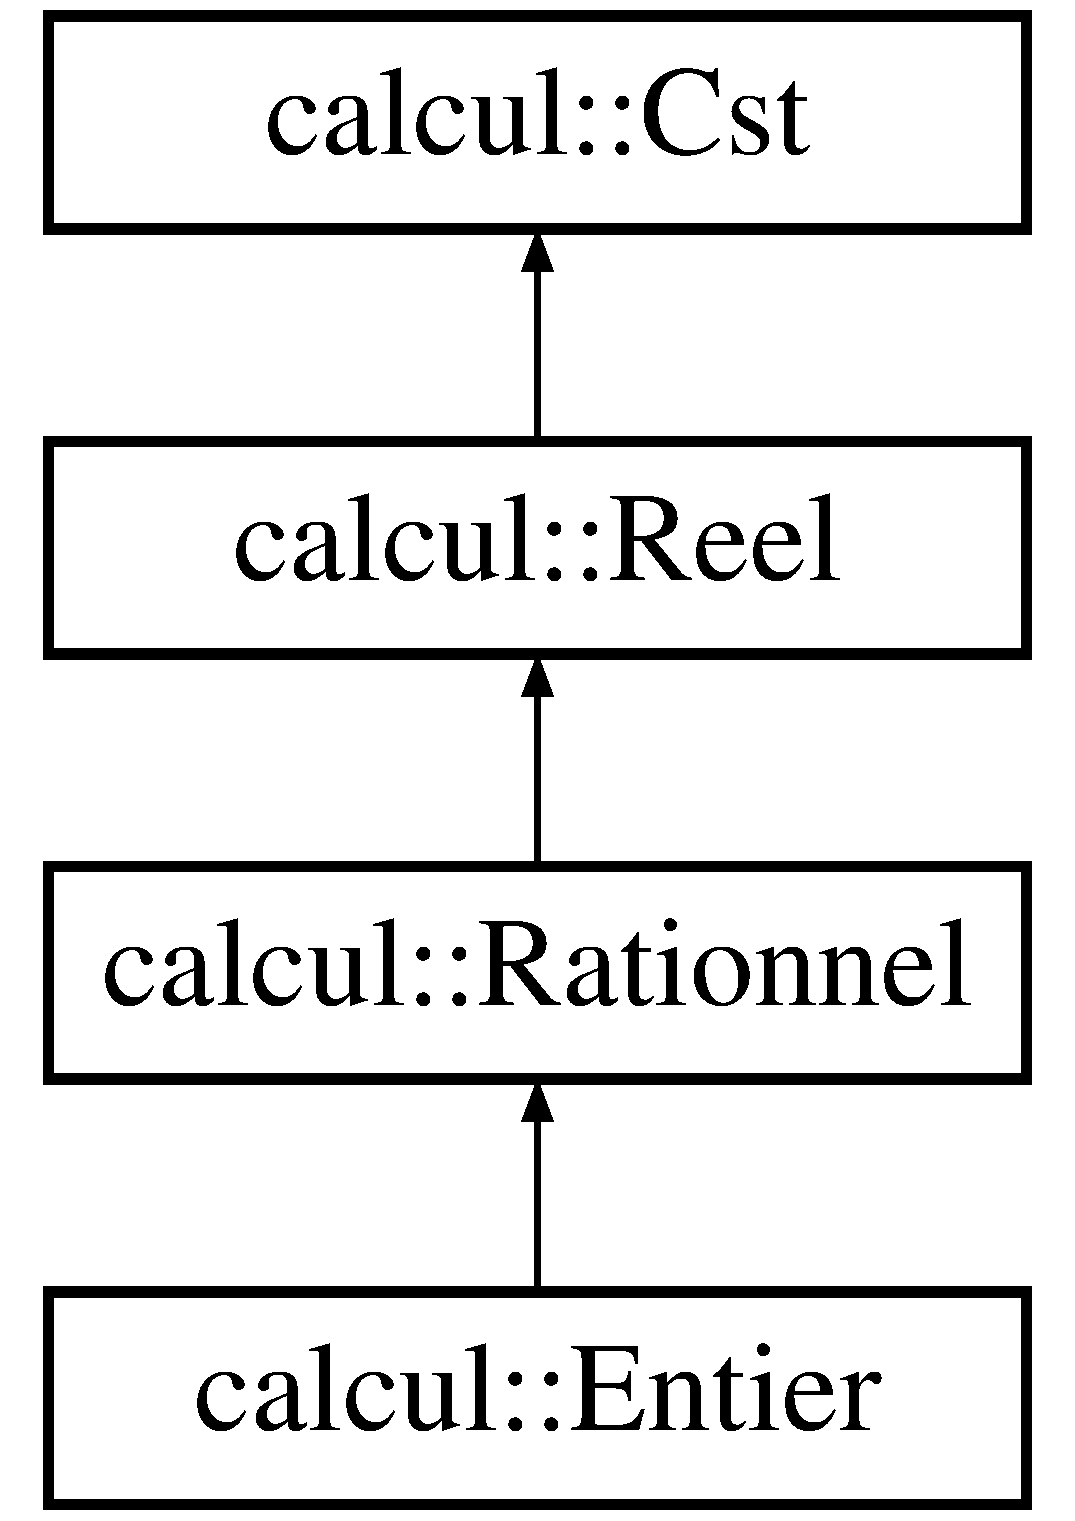
\includegraphics[height=4.000000cm]{classcalcul_1_1_rationnel}
\end{center}
\end{figure}
\subsection*{Fonctions membres publiques}
\begin{DoxyCompactItemize}
\item 
\hyperlink{classcalcul_1_1_rationnel_a56a577ec24723185aa6c133b1f3e6021}{Rationnel} (int num=0, int den=1)
\begin{DoxyCompactList}\small\item\em Constructeur par défaut de la classe \hyperlink{classcalcul_1_1_rationnel}{Rationnel}. \end{DoxyCompactList}\item 
\hypertarget{classcalcul_1_1_rationnel_a12ee060e5fca5f4291b222983d727268}{void \hyperlink{classcalcul_1_1_rationnel_a12ee060e5fca5f4291b222983d727268}{simplifier} ()}\label{classcalcul_1_1_rationnel_a12ee060e5fca5f4291b222983d727268}

\begin{DoxyCompactList}\small\item\em Méthode de simplification de la constante rationnelle. \end{DoxyCompactList}\item 
\hypertarget{classcalcul_1_1_rationnel_ac9596f5d24cef6120c0cabcd7923aa29}{int {\bfseries get\-Num} () const }\label{classcalcul_1_1_rationnel_ac9596f5d24cef6120c0cabcd7923aa29}

\item 
\hypertarget{classcalcul_1_1_rationnel_a6162bd26152763675e2fd1cf8fef792a}{int {\bfseries get\-Den} () const }\label{classcalcul_1_1_rationnel_a6162bd26152763675e2fd1cf8fef792a}

\item 
\hypertarget{classcalcul_1_1_rationnel_af9915c3a9b750c89533673b74f490f58}{\hyperlink{classcalcul_1_1_rationnel}{Rationnel} \& {\bfseries operator+} (const \hyperlink{classcalcul_1_1_cst}{Cst} \&other) const }\label{classcalcul_1_1_rationnel_af9915c3a9b750c89533673b74f490f58}

\item 
\hypertarget{classcalcul_1_1_rationnel_a0f4ab960d4323edbd7b91ab1e01f7f06}{\hyperlink{classcalcul_1_1_rationnel}{Rationnel} \& {\bfseries operator$\ast$} (const \hyperlink{classcalcul_1_1_cst}{Cst} \&other) const }\label{classcalcul_1_1_rationnel_a0f4ab960d4323edbd7b91ab1e01f7f06}

\item 
\hypertarget{classcalcul_1_1_rationnel_a33fea126a3f9dd73765e34e73c2ad5ad}{\hyperlink{classcalcul_1_1_rationnel}{Rationnel} \& {\bfseries operator-\/} (const \hyperlink{classcalcul_1_1_cst}{Cst} \&other) const }\label{classcalcul_1_1_rationnel_a33fea126a3f9dd73765e34e73c2ad5ad}

\item 
\hypertarget{classcalcul_1_1_rationnel_a1bf5fb5019a94907d469f49087ec1748}{\hyperlink{classcalcul_1_1_rationnel}{Rationnel} \& {\bfseries operator/} (const \hyperlink{classcalcul_1_1_cst}{Cst} \&other) const }\label{classcalcul_1_1_rationnel_a1bf5fb5019a94907d469f49087ec1748}

\item 
\hypertarget{classcalcul_1_1_rationnel_a225e9add04a23ec513ceac6375d91295}{\hyperlink{classcalcul_1_1_rationnel}{Rationnel} \& {\bfseries P\-O\-W} (const \hyperlink{classcalcul_1_1_cst}{Cst} \&other) const }\label{classcalcul_1_1_rationnel_a225e9add04a23ec513ceac6375d91295}

\item 
\hypertarget{classcalcul_1_1_rationnel_a61a6f4d83a90a770fe4bfdea3d5aab78}{\hyperlink{classcalcul_1_1_rationnel}{Rationnel} \& {\bfseries M\-O\-D} (const \hyperlink{classcalcul_1_1_cst}{Cst} \&other) const }\label{classcalcul_1_1_rationnel_a61a6f4d83a90a770fe4bfdea3d5aab78}

\item 
\hypertarget{classcalcul_1_1_rationnel_aa885cdb90dd48109b21d63a6245f20cb}{\hyperlink{classcalcul_1_1_rationnel}{Rationnel} \& {\bfseries S\-Q\-R} () const }\label{classcalcul_1_1_rationnel_aa885cdb90dd48109b21d63a6245f20cb}

\item 
\hypertarget{classcalcul_1_1_rationnel_a269ad60d4b8f0a26f3ddecb71d3cd9dd}{\hyperlink{classcalcul_1_1_rationnel}{Rationnel} \& {\bfseries C\-U\-B\-E} () const }\label{classcalcul_1_1_rationnel_a269ad60d4b8f0a26f3ddecb71d3cd9dd}

\item 
\hypertarget{classcalcul_1_1_rationnel_abfcd9f8855acd8561efad5d7bf07f6dd}{\hyperlink{classcalcul_1_1_rationnel}{Rationnel} \& {\bfseries S\-I\-G\-N} () const }\label{classcalcul_1_1_rationnel_abfcd9f8855acd8561efad5d7bf07f6dd}

\item 
\hypertarget{classcalcul_1_1_rationnel_ad055ff3bd58025eaf43dfe175cbf7120}{\hyperlink{classcalcul_1_1_rationnel}{Rationnel} \& {\bfseries S\-I\-N} (Angle\-Type angle=Degre) const }\label{classcalcul_1_1_rationnel_ad055ff3bd58025eaf43dfe175cbf7120}

\item 
\hypertarget{classcalcul_1_1_rationnel_ac137d2824084d6604399c40956f367e4}{\hyperlink{classcalcul_1_1_rationnel}{Rationnel} \& {\bfseries C\-O\-S} (Angle\-Type angle=Degre) const }\label{classcalcul_1_1_rationnel_ac137d2824084d6604399c40956f367e4}

\item 
\hypertarget{classcalcul_1_1_rationnel_a52e45c2883c62846a12ee456e1607591}{\hyperlink{classcalcul_1_1_rationnel}{Rationnel} \& {\bfseries T\-A\-N} (Angle\-Type angle=Degre) const }\label{classcalcul_1_1_rationnel_a52e45c2883c62846a12ee456e1607591}

\item 
\hypertarget{classcalcul_1_1_rationnel_a64330c0641aaffbf46e210f22eb6dfbe}{\hyperlink{classcalcul_1_1_rationnel}{Rationnel} \& {\bfseries S\-I\-N\-H} () const }\label{classcalcul_1_1_rationnel_a64330c0641aaffbf46e210f22eb6dfbe}

\item 
\hypertarget{classcalcul_1_1_rationnel_a9d217a858f5c99909990aecd691af613}{\hyperlink{classcalcul_1_1_rationnel}{Rationnel} \& {\bfseries C\-O\-S\-H} () const }\label{classcalcul_1_1_rationnel_a9d217a858f5c99909990aecd691af613}

\item 
\hypertarget{classcalcul_1_1_rationnel_a3dc7f10c84d8959224fd3169dabb1710}{\hyperlink{classcalcul_1_1_rationnel}{Rationnel} \& {\bfseries T\-A\-N\-H} () const }\label{classcalcul_1_1_rationnel_a3dc7f10c84d8959224fd3169dabb1710}

\item 
\hypertarget{classcalcul_1_1_rationnel_a102b3508ccc845619b56184415728e4f}{\hyperlink{classcalcul_1_1_rationnel}{Rationnel} \& {\bfseries L\-N} () const }\label{classcalcul_1_1_rationnel_a102b3508ccc845619b56184415728e4f}

\item 
\hypertarget{classcalcul_1_1_rationnel_a7574e317b50aa38d9bfc4ddee7825962}{\hyperlink{classcalcul_1_1_rationnel}{Rationnel} \& {\bfseries L\-O\-G} () const }\label{classcalcul_1_1_rationnel_a7574e317b50aa38d9bfc4ddee7825962}

\item 
\hypertarget{classcalcul_1_1_rationnel_a7d67ee2e809c403c1a615b657b830821}{\hyperlink{classcalcul_1_1_rationnel}{Rationnel} \& {\bfseries S\-Q\-R\-T} () const }\label{classcalcul_1_1_rationnel_a7d67ee2e809c403c1a615b657b830821}

\item 
\hypertarget{classcalcul_1_1_rationnel_a54455b17dbd3bc0d7ec6c606fcb07d32}{\hyperlink{classcalcul_1_1_rationnel}{Rationnel} \& {\bfseries I\-N\-V} () const }\label{classcalcul_1_1_rationnel_a54455b17dbd3bc0d7ec6c606fcb07d32}

\item 
\hypertarget{classcalcul_1_1_rationnel_a6dc7c90310d104125af60e4a8e6071b4}{\hyperlink{classcalcul_1_1_rationnel}{Rationnel} \& {\bfseries F\-A\-C\-T} () const }\label{classcalcul_1_1_rationnel_a6dc7c90310d104125af60e4a8e6071b4}

\item 
\hypertarget{classcalcul_1_1_rationnel_ab1c3ea55954724351cd2757ba389cf68}{\hyperlink{classcalcul_1_1_rationnel}{Rationnel} \& {\bfseries E\-V\-A\-L} () const }\label{classcalcul_1_1_rationnel_ab1c3ea55954724351cd2757ba389cf68}

\end{DoxyCompactItemize}
\subsection*{Fonctions membres protégées}
\begin{DoxyCompactItemize}
\item 
\hypertarget{classcalcul_1_1_rationnel_a1837ff66ec2f2c830c49727b4b5d5195}{void {\bfseries set\-String} ()}\label{classcalcul_1_1_rationnel_a1837ff66ec2f2c830c49727b4b5d5195}

\item 
\hypertarget{classcalcul_1_1_rationnel_a2470cf57b0d504e93fead66c317103ad}{int {\bfseries P\-G\-C\-D} (int a, int b)}\label{classcalcul_1_1_rationnel_a2470cf57b0d504e93fead66c317103ad}

\end{DoxyCompactItemize}
\subsection*{Attributs protégés}
\begin{DoxyCompactItemize}
\item 
\hypertarget{classcalcul_1_1_rationnel_a00ed21dd5e19ec08b32a3675d5210013}{int {\bfseries den}}\label{classcalcul_1_1_rationnel_a00ed21dd5e19ec08b32a3675d5210013}

\end{DoxyCompactItemize}


\subsection{Description détaillée}
Classe \hyperlink{classcalcul_1_1_rationnel}{Rationnel} représentant toutes les constantes rationnelles, hérite de la classe \hyperlink{classcalcul_1_1_reel}{Reel}. 

\subsection{Documentation des constructeurs et destructeur}
\hypertarget{classcalcul_1_1_rationnel_a56a577ec24723185aa6c133b1f3e6021}{\index{calcul\-::\-Rationnel@{calcul\-::\-Rationnel}!Rationnel@{Rationnel}}
\index{Rationnel@{Rationnel}!calcul::Rationnel@{calcul\-::\-Rationnel}}
\subsubsection[{Rationnel}]{\setlength{\rightskip}{0pt plus 5cm}calcul\-::\-Rationnel\-::\-Rationnel (
\begin{DoxyParamCaption}
\item[{int}]{num = {\ttfamily 0}, }
\item[{int}]{den = {\ttfamily 1}}
\end{DoxyParamCaption}
)\hspace{0.3cm}{\ttfamily [inline]}}}\label{classcalcul_1_1_rationnel_a56a577ec24723185aa6c133b1f3e6021}


Constructeur par défaut de la classe \hyperlink{classcalcul_1_1_rationnel}{Rationnel}. 


\begin{DoxyParams}{Paramètres}
{\em num} & \-: Valeur du numérateur \\
\hline
{\em den} & \-: Valeur du dénominateur \\
\hline
\end{DoxyParams}


La documentation de cette classe a été générée à partir des fichiers suivants \-:\begin{DoxyCompactItemize}
\item 
C\-:/\-Users/\-William/\-Dropbox/lo21/projet/\-Projet/cst.\-h\item 
C\-:/\-Users/\-William/\-Dropbox/lo21/projet/\-Projet/cst.\-cpp\end{DoxyCompactItemize}

\hypertarget{classcalcul_1_1_reel}{\section{Référence de la classe calcul\-:\-:Reel}
\label{classcalcul_1_1_reel}\index{calcul\-::\-Reel@{calcul\-::\-Reel}}
}


Classe \hyperlink{classcalcul_1_1_reel}{Reel} représentant toutes les constantes réelles.  




{\ttfamily \#include $<$cst.\-h$>$}

Graphe d'héritage de calcul\-:\-:Reel\-:\begin{figure}[H]
\begin{center}
\leavevmode
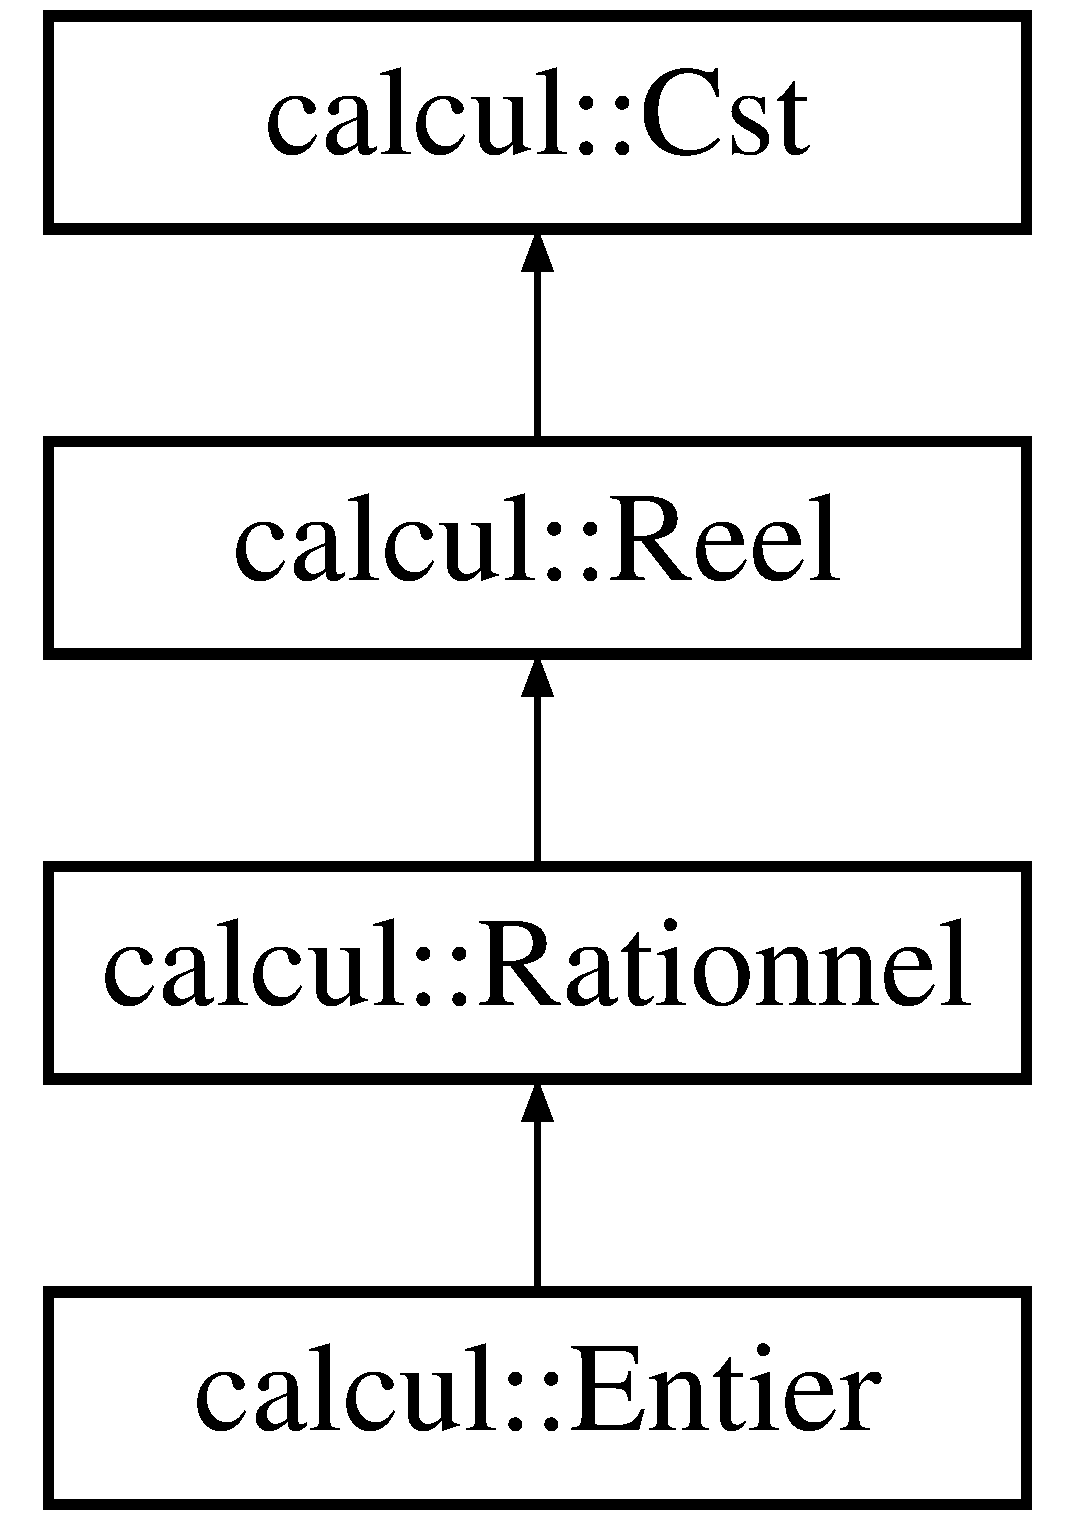
\includegraphics[height=4.000000cm]{classcalcul_1_1_reel}
\end{center}
\end{figure}
\subsection*{Fonctions membres publiques}
\begin{DoxyCompactItemize}
\item 
\hypertarget{classcalcul_1_1_reel_ae506e14392d2949f515c6371b8c99966}{bool {\bfseries is\-Number} () const }\label{classcalcul_1_1_reel_ae506e14392d2949f515c6371b8c99966}

\item 
double \hyperlink{classcalcul_1_1_reel_a6412ad4d84dcd302c1fae1f7ec3ede46}{get\-Valeur} () const 
\begin{DoxyCompactList}\small\item\em Récupérer la valeur de la constante. \end{DoxyCompactList}\item 
\hyperlink{classcalcul_1_1_reel_a280d3cbf64344c09f6a4a652fcab3463}{Reel} (double valeur=0)
\begin{DoxyCompactList}\small\item\em Constructeur par défaut de la classe \hyperlink{classcalcul_1_1_reel}{Reel}. \end{DoxyCompactList}\item 
\hypertarget{classcalcul_1_1_reel_a1538ddbfb6025e198b677a94458da685}{\hyperlink{classcalcul_1_1_reel}{Reel} \& {\bfseries operator+} (const \hyperlink{classcalcul_1_1_cst}{Cst} \&other) const }\label{classcalcul_1_1_reel_a1538ddbfb6025e198b677a94458da685}

\item 
\hypertarget{classcalcul_1_1_reel_a9a0cc280b8a1b31c312cd9a607e0ca6f}{\hyperlink{classcalcul_1_1_reel}{Reel} \& {\bfseries operator$\ast$} (const \hyperlink{classcalcul_1_1_cst}{Cst} \&other) const }\label{classcalcul_1_1_reel_a9a0cc280b8a1b31c312cd9a607e0ca6f}

\item 
\hypertarget{classcalcul_1_1_reel_a6429fb315d620acec8c79852a6f25a6f}{\hyperlink{classcalcul_1_1_reel}{Reel} \& {\bfseries operator-\/} (const \hyperlink{classcalcul_1_1_cst}{Cst} \&other) const }\label{classcalcul_1_1_reel_a6429fb315d620acec8c79852a6f25a6f}

\item 
\hypertarget{classcalcul_1_1_reel_ae7131d5efb1995804fdcf3ac9c201540}{\hyperlink{classcalcul_1_1_reel}{Reel} \& {\bfseries operator/} (const \hyperlink{classcalcul_1_1_cst}{Cst} \&other) const }\label{classcalcul_1_1_reel_ae7131d5efb1995804fdcf3ac9c201540}

\item 
\hypertarget{classcalcul_1_1_reel_a4fa85a19bb509c7a7a83d45fd801b073}{\hyperlink{classcalcul_1_1_reel}{Reel} \& {\bfseries P\-O\-W} (const \hyperlink{classcalcul_1_1_cst}{Cst} \&other) const }\label{classcalcul_1_1_reel_a4fa85a19bb509c7a7a83d45fd801b073}

\item 
\hypertarget{classcalcul_1_1_reel_a78b0d9a9a43bafc804dcf1fb98cf1541}{\hyperlink{classcalcul_1_1_reel}{Reel} \& {\bfseries M\-O\-D} (const \hyperlink{classcalcul_1_1_cst}{Cst} \&other) const }\label{classcalcul_1_1_reel_a78b0d9a9a43bafc804dcf1fb98cf1541}

\item 
\hypertarget{classcalcul_1_1_reel_a7319b067da3be640441f02b8056276d8}{\hyperlink{classcalcul_1_1_reel}{Reel} \& {\bfseries S\-Q\-R} () const }\label{classcalcul_1_1_reel_a7319b067da3be640441f02b8056276d8}

\item 
\hypertarget{classcalcul_1_1_reel_a880b14440a1909babf58c66cb22e1b66}{\hyperlink{classcalcul_1_1_reel}{Reel} \& {\bfseries C\-U\-B\-E} () const }\label{classcalcul_1_1_reel_a880b14440a1909babf58c66cb22e1b66}

\item 
\hypertarget{classcalcul_1_1_reel_a351abfa7f5e3f7e7999c0d4db3856c7c}{\hyperlink{classcalcul_1_1_reel}{Reel} \& {\bfseries S\-I\-G\-N} () const }\label{classcalcul_1_1_reel_a351abfa7f5e3f7e7999c0d4db3856c7c}

\item 
\hypertarget{classcalcul_1_1_reel_af3866131110c0ebcf15248bba9eab968}{\hyperlink{classcalcul_1_1_reel}{Reel} \& {\bfseries S\-I\-N} (Angle\-Type angle=Degre) const }\label{classcalcul_1_1_reel_af3866131110c0ebcf15248bba9eab968}

\item 
\hypertarget{classcalcul_1_1_reel_acd95fc792dac0834a6c63a3f61972b05}{\hyperlink{classcalcul_1_1_reel}{Reel} \& {\bfseries C\-O\-S} (Angle\-Type angle=Degre) const }\label{classcalcul_1_1_reel_acd95fc792dac0834a6c63a3f61972b05}

\item 
\hypertarget{classcalcul_1_1_reel_aca72f105d4c151b9b7b7809b8b073d01}{\hyperlink{classcalcul_1_1_reel}{Reel} \& {\bfseries T\-A\-N} (Angle\-Type angle=Degre) const }\label{classcalcul_1_1_reel_aca72f105d4c151b9b7b7809b8b073d01}

\item 
\hypertarget{classcalcul_1_1_reel_a7bcdbc024fa984885ad6d11b9b9b7498}{\hyperlink{classcalcul_1_1_reel}{Reel} \& {\bfseries S\-I\-N\-H} () const }\label{classcalcul_1_1_reel_a7bcdbc024fa984885ad6d11b9b9b7498}

\item 
\hypertarget{classcalcul_1_1_reel_a1c302e4b68d9e617024cdb4cb26205c5}{\hyperlink{classcalcul_1_1_reel}{Reel} \& {\bfseries C\-O\-S\-H} () const }\label{classcalcul_1_1_reel_a1c302e4b68d9e617024cdb4cb26205c5}

\item 
\hypertarget{classcalcul_1_1_reel_a84d981dad734ac55b0de24876c210c6b}{\hyperlink{classcalcul_1_1_reel}{Reel} \& {\bfseries T\-A\-N\-H} () const }\label{classcalcul_1_1_reel_a84d981dad734ac55b0de24876c210c6b}

\item 
\hypertarget{classcalcul_1_1_reel_a5fa6c5d205b852093157f1f86cd4bb68}{\hyperlink{classcalcul_1_1_reel}{Reel} \& {\bfseries L\-N} () const }\label{classcalcul_1_1_reel_a5fa6c5d205b852093157f1f86cd4bb68}

\item 
\hypertarget{classcalcul_1_1_reel_ac22982827f92a9c044e8b0a5e594929e}{\hyperlink{classcalcul_1_1_reel}{Reel} \& {\bfseries L\-O\-G} () const }\label{classcalcul_1_1_reel_ac22982827f92a9c044e8b0a5e594929e}

\item 
\hypertarget{classcalcul_1_1_reel_a4afb261cb350db25f692bc39d8645c69}{\hyperlink{classcalcul_1_1_reel}{Reel} \& {\bfseries S\-Q\-R\-T} () const }\label{classcalcul_1_1_reel_a4afb261cb350db25f692bc39d8645c69}

\item 
\hypertarget{classcalcul_1_1_reel_ac704df6ace45a561847e3a881768614b}{\hyperlink{classcalcul_1_1_reel}{Reel} \& {\bfseries I\-N\-V} () const }\label{classcalcul_1_1_reel_ac704df6ace45a561847e3a881768614b}

\item 
\hypertarget{classcalcul_1_1_reel_ae370422a6024657880a5f650f668c91f}{\hyperlink{classcalcul_1_1_reel}{Reel} \& {\bfseries F\-A\-C\-T} () const }\label{classcalcul_1_1_reel_ae370422a6024657880a5f650f668c91f}

\item 
\hypertarget{classcalcul_1_1_reel_afce90d98cc806db427d2561b949de170}{\hyperlink{classcalcul_1_1_reel}{Reel} \& {\bfseries E\-V\-A\-L} () const }\label{classcalcul_1_1_reel_afce90d98cc806db427d2561b949de170}

\end{DoxyCompactItemize}
\subsection*{Fonctions membres protégées}
\begin{DoxyCompactItemize}
\item 
\hypertarget{classcalcul_1_1_reel_a667dde4c69dee28d6de312fa2a1411b6}{void {\bfseries set\-String} ()}\label{classcalcul_1_1_reel_a667dde4c69dee28d6de312fa2a1411b6}

\end{DoxyCompactItemize}
\subsection*{Attributs protégés}
\begin{DoxyCompactItemize}
\item 
\hypertarget{classcalcul_1_1_reel_a9d50ca5e60d0ad3604537bb6892a9902}{double {\bfseries valeur}}\label{classcalcul_1_1_reel_a9d50ca5e60d0ad3604537bb6892a9902}

\end{DoxyCompactItemize}


\subsection{Description détaillée}
Classe \hyperlink{classcalcul_1_1_reel}{Reel} représentant toutes les constantes réelles. 

\subsection{Documentation des constructeurs et destructeur}
\hypertarget{classcalcul_1_1_reel_a280d3cbf64344c09f6a4a652fcab3463}{\index{calcul\-::\-Reel@{calcul\-::\-Reel}!Reel@{Reel}}
\index{Reel@{Reel}!calcul::Reel@{calcul\-::\-Reel}}
\subsubsection[{Reel}]{\setlength{\rightskip}{0pt plus 5cm}calcul\-::\-Reel\-::\-Reel (
\begin{DoxyParamCaption}
\item[{double}]{valeur = {\ttfamily 0}}
\end{DoxyParamCaption}
)\hspace{0.3cm}{\ttfamily [inline]}}}\label{classcalcul_1_1_reel_a280d3cbf64344c09f6a4a652fcab3463}


Constructeur par défaut de la classe \hyperlink{classcalcul_1_1_reel}{Reel}. 


\begin{DoxyParams}{Paramètres}
{\em valeur} & \-: Valeur de la constante réelled \\
\hline
\end{DoxyParams}


\subsection{Documentation des fonctions membres}
\hypertarget{classcalcul_1_1_reel_a6412ad4d84dcd302c1fae1f7ec3ede46}{\index{calcul\-::\-Reel@{calcul\-::\-Reel}!get\-Valeur@{get\-Valeur}}
\index{get\-Valeur@{get\-Valeur}!calcul::Reel@{calcul\-::\-Reel}}
\subsubsection[{get\-Valeur}]{\setlength{\rightskip}{0pt plus 5cm}double Reel\-::get\-Valeur (
\begin{DoxyParamCaption}
{}
\end{DoxyParamCaption}
) const\hspace{0.3cm}{\ttfamily [virtual]}}}\label{classcalcul_1_1_reel_a6412ad4d84dcd302c1fae1f7ec3ede46}


Récupérer la valeur de la constante. 

\begin{DoxyReturn}{Renvoie}
La valeur en double 
\end{DoxyReturn}


Réimplémentée à partir de \hyperlink{classcalcul_1_1_cst}{calcul\-::\-Cst}.



La documentation de cette classe a été générée à partir des fichiers suivants \-:\begin{DoxyCompactItemize}
\item 
C\-:/\-Users/\-William/\-Dropbox/lo21/projet/\-Projet/cst.\-h\item 
C\-:/\-Users/\-William/\-Dropbox/lo21/projet/\-Projet/cst.\-cpp\end{DoxyCompactItemize}

\hypertarget{class_ui___widget}{\section{Référence de la classe Ui\-\_\-\-Widget}
\label{class_ui___widget}\index{Ui\-\_\-\-Widget@{Ui\-\_\-\-Widget}}
}
Graphe d'héritage de Ui\-\_\-\-Widget\-:\begin{figure}[H]
\begin{center}
\leavevmode
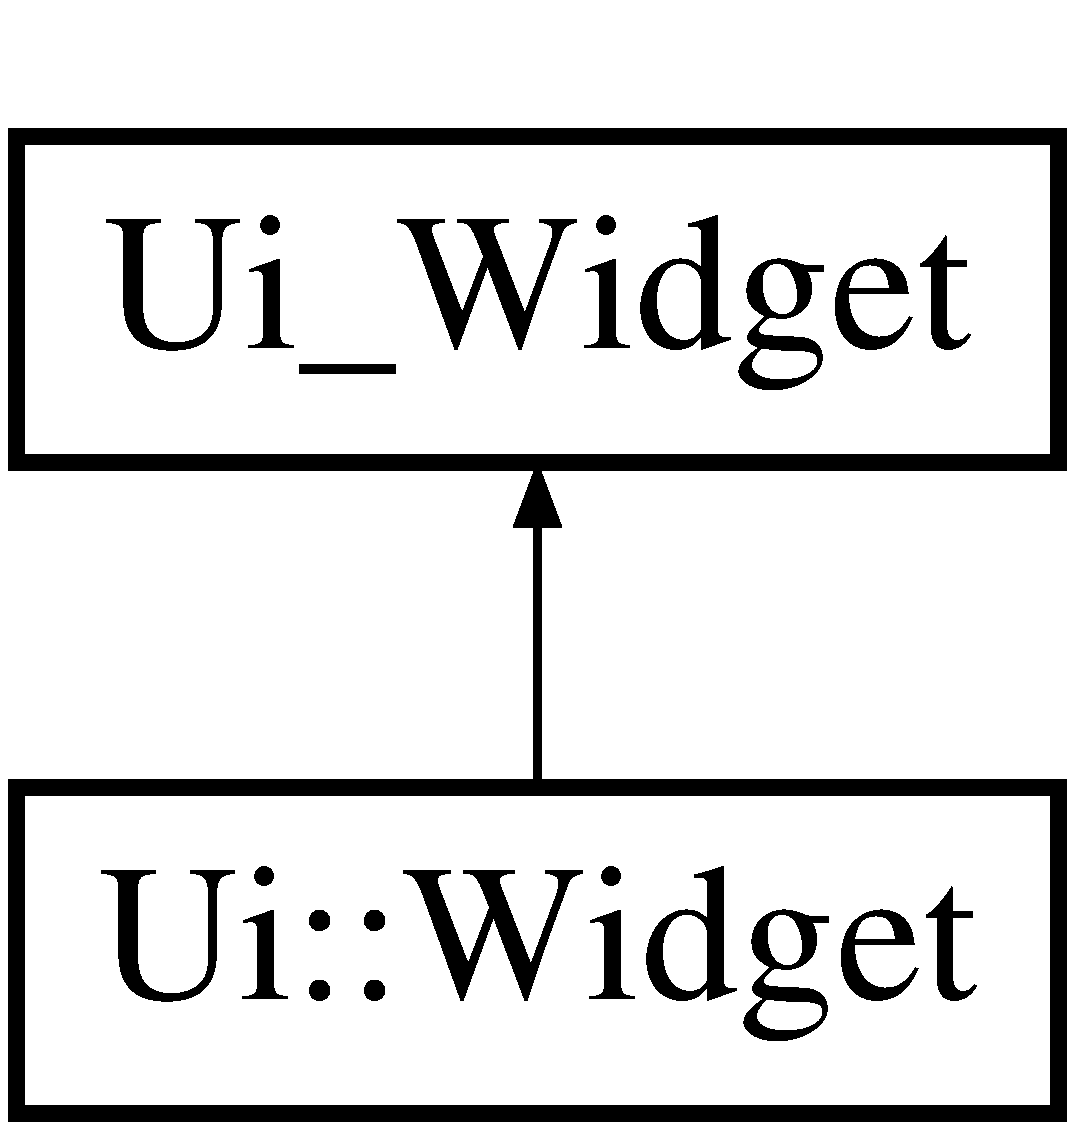
\includegraphics[height=2.000000cm]{class_ui___widget}
\end{center}
\end{figure}
\subsection*{Fonctions membres publiques}
\begin{DoxyCompactItemize}
\item 
\hypertarget{class_ui___widget_a9039ed8704971418cbe19ef8c9eea266}{void {\bfseries setup\-Ui} (Q\-Widget $\ast$Widget)}\label{class_ui___widget_a9039ed8704971418cbe19ef8c9eea266}

\item 
\hypertarget{class_ui___widget_ae1cb85db8d3658df8dcd104361edcecb}{void {\bfseries retranslate\-Ui} (Q\-Widget $\ast$Widget)}\label{class_ui___widget_ae1cb85db8d3658df8dcd104361edcecb}

\end{DoxyCompactItemize}
\subsection*{Attributs publics}
\begin{DoxyCompactItemize}
\item 
\hypertarget{class_ui___widget_a5ca3416e2d3b45799260113206bce5d2}{Q\-Tool\-Bar $\ast$ {\bfseries main\-Tool\-Bar}}\label{class_ui___widget_a5ca3416e2d3b45799260113206bce5d2}

\item 
\hypertarget{class_ui___widget_a0616d9c4a5af2cb76046e822a7fcfc9a}{Q\-Status\-Bar $\ast$ {\bfseries status\-Bar}}\label{class_ui___widget_a0616d9c4a5af2cb76046e822a7fcfc9a}

\item 
\hypertarget{class_ui___widget_a0562d1871ab799c677b56f36f345c6dd}{Q\-Group\-Box $\ast$ {\bfseries group\-Box\-\_\-4}}\label{class_ui___widget_a0562d1871ab799c677b56f36f345c6dd}

\item 
\hypertarget{class_ui___widget_a39cbbadb241d2b4af7b8f912a591b481}{Q\-Radio\-Button $\ast$ {\bfseries \-\_\-mod\-Complexe\-O\-N}}\label{class_ui___widget_a39cbbadb241d2b4af7b8f912a591b481}

\item 
\hypertarget{class_ui___widget_a249b531b400ff8efa687037f75d8d7c0}{Q\-Radio\-Button $\ast$ {\bfseries \-\_\-mod\-Complexe\-O\-F\-F}}\label{class_ui___widget_a249b531b400ff8efa687037f75d8d7c0}

\item 
\hypertarget{class_ui___widget_ac164b5fb7882f7943de7a8e441487a61}{Q\-Group\-Box $\ast$ {\bfseries group\-Box\-\_\-2}}\label{class_ui___widget_ac164b5fb7882f7943de7a8e441487a61}

\item 
\hypertarget{class_ui___widget_a840a8431d2528e6237f563a8b69efd33}{Q\-Radio\-Button $\ast$ {\bfseries \-\_\-mod\-Entiers}}\label{class_ui___widget_a840a8431d2528e6237f563a8b69efd33}

\item 
\hypertarget{class_ui___widget_a56279ab34310f87e7846fc03f45f4499}{Q\-Radio\-Button $\ast$ {\bfseries \-\_\-mod\-Rationnels}}\label{class_ui___widget_a56279ab34310f87e7846fc03f45f4499}

\item 
\hypertarget{class_ui___widget_ade3f0e823929ba818460a8c5fb4b153c}{Q\-Radio\-Button $\ast$ {\bfseries \-\_\-mod\-Reels}}\label{class_ui___widget_ade3f0e823929ba818460a8c5fb4b153c}

\item 
\hypertarget{class_ui___widget_a37b5f02d18b7fc93109cab8edb481367}{Q\-Group\-Box $\ast$ {\bfseries group\-Box\-\_\-3}}\label{class_ui___widget_a37b5f02d18b7fc93109cab8edb481367}

\item 
\hypertarget{class_ui___widget_ac82b42eb4da7229f87901b85b7c6d129}{Q\-Check\-Box $\ast$ {\bfseries \-\_\-clavier\-Basic}}\label{class_ui___widget_ac82b42eb4da7229f87901b85b7c6d129}

\item 
\hypertarget{class_ui___widget_a02b6251446644654ed84730c3f36b5f7}{Q\-Check\-Box $\ast$ {\bfseries \-\_\-clavier\-Avance}}\label{class_ui___widget_a02b6251446644654ed84730c3f36b5f7}

\item 
\hypertarget{class_ui___widget_a6f47c316a7b69f07a2af17530c8d4f7a}{Q\-Widget $\ast$ {\bfseries grid\-Layout\-Widget}}\label{class_ui___widget_a6f47c316a7b69f07a2af17530c8d4f7a}

\item 
\hypertarget{class_ui___widget_acf97a903ccaf262fd2920ab3e3bd1e96}{Q\-Grid\-Layout $\ast$ {\bfseries grid\-Layout}}\label{class_ui___widget_acf97a903ccaf262fd2920ab3e3bd1e96}

\item 
\hypertarget{class_ui___widget_a73bad0f249f5a610e9def06aa8608307}{Q\-Push\-Button $\ast$ {\bfseries Button7}}\label{class_ui___widget_a73bad0f249f5a610e9def06aa8608307}

\item 
\hypertarget{class_ui___widget_a28face08d0c94b91dbc203dd03583105}{Q\-Push\-Button $\ast$ {\bfseries Button8}}\label{class_ui___widget_a28face08d0c94b91dbc203dd03583105}

\item 
\hypertarget{class_ui___widget_aad648f839cc8acf85cc977cd4bc95f2a}{Q\-Push\-Button $\ast$ {\bfseries Button9}}\label{class_ui___widget_aad648f839cc8acf85cc977cd4bc95f2a}

\item 
\hypertarget{class_ui___widget_a34a20a92c49032aa5481bb7ac4eef9be}{Q\-Push\-Button $\ast$ {\bfseries Button4}}\label{class_ui___widget_a34a20a92c49032aa5481bb7ac4eef9be}

\item 
\hypertarget{class_ui___widget_a0609a971dc82e6bd8be0d1afa1b6b871}{Q\-Push\-Button $\ast$ {\bfseries Button5}}\label{class_ui___widget_a0609a971dc82e6bd8be0d1afa1b6b871}

\item 
\hypertarget{class_ui___widget_aa4b2cc71337bf287757719716f667c7d}{Q\-Push\-Button $\ast$ {\bfseries Button6}}\label{class_ui___widget_aa4b2cc71337bf287757719716f667c7d}

\item 
\hypertarget{class_ui___widget_a8a753deffbf5c58f94726ba675845921}{Q\-Push\-Button $\ast$ {\bfseries Button1}}\label{class_ui___widget_a8a753deffbf5c58f94726ba675845921}

\item 
\hypertarget{class_ui___widget_a953d3410c29e27ef7d773fe324136dcc}{Q\-Push\-Button $\ast$ {\bfseries Button2}}\label{class_ui___widget_a953d3410c29e27ef7d773fe324136dcc}

\item 
\hypertarget{class_ui___widget_ae2076ab6042656ec55ea43e97078b9e8}{Q\-Push\-Button $\ast$ {\bfseries Button3}}\label{class_ui___widget_ae2076ab6042656ec55ea43e97078b9e8}

\item 
\hypertarget{class_ui___widget_a883310cc38bd22523436d437962ec502}{Q\-Push\-Button $\ast$ {\bfseries Button0}}\label{class_ui___widget_a883310cc38bd22523436d437962ec502}

\item 
\hypertarget{class_ui___widget_aa94e00656d550c536f6ee61024cd30af}{Q\-Push\-Button $\ast$ {\bfseries Buttonvirgule}}\label{class_ui___widget_aa94e00656d550c536f6ee61024cd30af}

\item 
\hypertarget{class_ui___widget_af134f4654c81de0e7680989471e1c9f4}{Q\-Push\-Button $\ast$ {\bfseries Buttonswap}}\label{class_ui___widget_af134f4654c81de0e7680989471e1c9f4}

\item 
\hypertarget{class_ui___widget_a4c2bbc690527ed4008f49afc2f9d617e}{Q\-Push\-Button $\ast$ {\bfseries Buttonmean}}\label{class_ui___widget_a4c2bbc690527ed4008f49afc2f9d617e}

\item 
\hypertarget{class_ui___widget_a5f498eecc44f6fc4d4a51894fc50029a}{Q\-Push\-Button $\ast$ {\bfseries Buttonln}}\label{class_ui___widget_a5f498eecc44f6fc4d4a51894fc50029a}

\item 
\hypertarget{class_ui___widget_abd2e2d2c83323770c42b80406532729f}{Q\-Push\-Button $\ast$ {\bfseries Buttonsinh}}\label{class_ui___widget_abd2e2d2c83323770c42b80406532729f}

\item 
\hypertarget{class_ui___widget_ab56226a4d2ae2676a2f91be639ba7189}{Q\-Push\-Button $\ast$ {\bfseries Buttonsin}}\label{class_ui___widget_ab56226a4d2ae2676a2f91be639ba7189}

\item 
\hypertarget{class_ui___widget_ad7743fbc29323db1351dd7720a51c852}{Q\-Push\-Button $\ast$ {\bfseries Buttoncosh}}\label{class_ui___widget_ad7743fbc29323db1351dd7720a51c852}

\item 
\hypertarget{class_ui___widget_a18c578cb6d47426ca4483f110056ecc6}{Q\-Push\-Button $\ast$ {\bfseries Buttontanh}}\label{class_ui___widget_a18c578cb6d47426ca4483f110056ecc6}

\item 
\hypertarget{class_ui___widget_ae3c6db1995e88385a356f048bc163457}{Q\-Push\-Button $\ast$ {\bfseries Buttontan}}\label{class_ui___widget_ae3c6db1995e88385a356f048bc163457}

\item 
\hypertarget{class_ui___widget_a52f58c5429fd5a3830db935b14b39c59}{Q\-Push\-Button $\ast$ {\bfseries Buttoncos}}\label{class_ui___widget_a52f58c5429fd5a3830db935b14b39c59}

\item 
\hypertarget{class_ui___widget_a77be7ca86bc99ede815a683a218ec9b2}{Q\-Push\-Button $\ast$ {\bfseries Buttonmod}}\label{class_ui___widget_a77be7ca86bc99ede815a683a218ec9b2}

\item 
\hypertarget{class_ui___widget_a496728025de61e51212251919772f5da}{Q\-Push\-Button $\ast$ {\bfseries Buttonxy}}\label{class_ui___widget_a496728025de61e51212251919772f5da}

\item 
\hypertarget{class_ui___widget_ae256ccaff93a97cf16b47da729e7d6df}{Q\-Push\-Button $\ast$ {\bfseries Buttonx2}}\label{class_ui___widget_ae256ccaff93a97cf16b47da729e7d6df}

\item 
\hypertarget{class_ui___widget_a0041ca856c16cce95a9671af4207d0aa}{Q\-Push\-Button $\ast$ {\bfseries Buttonx3}}\label{class_ui___widget_a0041ca856c16cce95a9671af4207d0aa}

\item 
\hypertarget{class_ui___widget_a1bf023784eccad419b1795134a512d2b}{Q\-Push\-Button $\ast$ {\bfseries Buttonsum}}\label{class_ui___widget_a1bf023784eccad419b1795134a512d2b}

\item 
\hypertarget{class_ui___widget_acd65cbee11a5aecfe0e234b10ee9c261}{Q\-Push\-Button $\ast$ {\bfseries Buttondollar}}\label{class_ui___widget_acd65cbee11a5aecfe0e234b10ee9c261}

\item 
\hypertarget{class_ui___widget_a45b10b1f43ac4c6ee9b29547d9c45ecf}{Q\-Push\-Button $\ast$ {\bfseries Buttonplus}}\label{class_ui___widget_a45b10b1f43ac4c6ee9b29547d9c45ecf}

\item 
\hypertarget{class_ui___widget_ae73e92f13f04acb357c32c6ba7d5c64f}{Q\-Push\-Button $\ast$ {\bfseries Buttonmoins}}\label{class_ui___widget_ae73e92f13f04acb357c32c6ba7d5c64f}

\item 
\hypertarget{class_ui___widget_ae3fc3d9289910411ec905d7df51083ea}{Q\-Push\-Button $\ast$ {\bfseries Buttonfois}}\label{class_ui___widget_ae3fc3d9289910411ec905d7df51083ea}

\item 
\hypertarget{class_ui___widget_a2baccaa605ba05aed0065a0cd1c35ae3}{Q\-Push\-Button $\ast$ {\bfseries Buttondiviser}}\label{class_ui___widget_a2baccaa605ba05aed0065a0cd1c35ae3}

\item 
\hypertarget{class_ui___widget_a6c6c5c0b146d3e2498195d06d4b796e3}{Q\-Push\-Button $\ast$ {\bfseries Buttonlog}}\label{class_ui___widget_a6c6c5c0b146d3e2498195d06d4b796e3}

\item 
\hypertarget{class_ui___widget_aec0b5d2989e3722c9d8e9ace4b8f33d9}{Q\-Push\-Button $\ast$ {\bfseries Buttonfact}}\label{class_ui___widget_aec0b5d2989e3722c9d8e9ace4b8f33d9}

\item 
\hypertarget{class_ui___widget_ae522e2ca0543ccd827ce8ef51301f5f6}{Q\-Radio\-Button $\ast$ {\bfseries radio\-Buttonradian}}\label{class_ui___widget_ae522e2ca0543ccd827ce8ef51301f5f6}

\item 
\hypertarget{class_ui___widget_abf74b2656876727d8ea9340dd5d68838}{Q\-Radio\-Button $\ast$ {\bfseries radio\-Buttondegree}}\label{class_ui___widget_abf74b2656876727d8ea9340dd5d68838}

\item 
\hypertarget{class_ui___widget_abd0500e7ddcdf9f7912a4e5d699c557f}{Q\-Push\-Button $\ast$ {\bfseries Buttonapo}}\label{class_ui___widget_abd0500e7ddcdf9f7912a4e5d699c557f}

\item 
\hypertarget{class_ui___widget_a60c79c26e095f45e7a6f9a13dd53b065}{Q\-Push\-Button $\ast$ {\bfseries Buttondup}}\label{class_ui___widget_a60c79c26e095f45e7a6f9a13dd53b065}

\item 
\hypertarget{class_ui___widget_a7f645a453d9c6dacac995c67ce167937}{Q\-Push\-Button $\ast$ {\bfseries Buttondrop}}\label{class_ui___widget_a7f645a453d9c6dacac995c67ce167937}

\item 
\hypertarget{class_ui___widget_a29fdee99033f49a52242cd563393d8fd}{Q\-Push\-Button $\ast$ {\bfseries Buttonclear}}\label{class_ui___widget_a29fdee99033f49a52242cd563393d8fd}

\item 
\hypertarget{class_ui___widget_a3126b93450dcc18cede73b9d1ee7c6b0}{Q\-Label $\ast$ {\bfseries label}}\label{class_ui___widget_a3126b93450dcc18cede73b9d1ee7c6b0}

\item 
\hypertarget{class_ui___widget_aacb08d12203102e108d60ab2af782b41}{Q\-V\-Box\-Layout $\ast$ {\bfseries vertical\-Layout\-\_\-3}}\label{class_ui___widget_aacb08d12203102e108d60ab2af782b41}

\item 
\hypertarget{class_ui___widget_a4ae0ee832d9191ae0cd7f0e511cc14e2}{Q\-Line\-Edit $\ast$ {\bfseries line\-Edit}}\label{class_ui___widget_a4ae0ee832d9191ae0cd7f0e511cc14e2}

\item 
\hypertarget{class_ui___widget_a079d25cecd0331da3c930a1258f948d7}{Q\-Push\-Button $\ast$ {\bfseries Buttonenter}}\label{class_ui___widget_a079d25cecd0331da3c930a1258f948d7}

\item 
\hypertarget{class_ui___widget_a63eb2db09f8970557b49c468dd13e10b}{Q\-Text\-Edit $\ast$ {\bfseries Pile\-Calcul}}\label{class_ui___widget_a63eb2db09f8970557b49c468dd13e10b}

\item 
\hypertarget{class_ui___widget_abe2fa37c556f16b9f966898e33dc08d0}{Q\-Text\-Edit $\ast$ {\bfseries Pile\-Affichage}}\label{class_ui___widget_abe2fa37c556f16b9f966898e33dc08d0}

\item 
\hypertarget{class_ui___widget_a087952812244aa5a76507b00467569f2}{Q\-Push\-Button $\ast$ {\bfseries Buttonsqrt}}\label{class_ui___widget_a087952812244aa5a76507b00467569f2}

\item 
\hypertarget{class_ui___widget_a5d232270040cb01d5ecda5557c0ce372}{Q\-Push\-Button $\ast$ {\bfseries Buttonsign}}\label{class_ui___widget_a5d232270040cb01d5ecda5557c0ce372}

\item 
\hypertarget{class_ui___widget_a7794c8e94ed6a05b10005cbb3f128fe1}{Q\-Push\-Button $\ast$ {\bfseries Buttoninv}}\label{class_ui___widget_a7794c8e94ed6a05b10005cbb3f128fe1}

\item 
\hypertarget{class_ui___widget_a04cf1b7c4d01e5e9d0720c1782877a68}{Q\-Push\-Button $\ast$ {\bfseries Buttoneval}}\label{class_ui___widget_a04cf1b7c4d01e5e9d0720c1782877a68}

\item 
\hypertarget{class_ui___widget_a51b15ede6f8aa722585d9be06f9c92f8}{Q\-Push\-Button $\ast$ {\bfseries Buttonspace}}\label{class_ui___widget_a51b15ede6f8aa722585d9be06f9c92f8}

\item 
\hypertarget{class_ui___widget_adfcab5569ac08da197e14dba01390755}{Q\-Label $\ast$ {\bfseries label\-\_\-3}}\label{class_ui___widget_adfcab5569ac08da197e14dba01390755}

\item 
\hypertarget{class_ui___widget_a6f06b143349464b5b19ac0ffe2fc084d}{Q\-Label $\ast$ {\bfseries label\-\_\-2}}\label{class_ui___widget_a6f06b143349464b5b19ac0ffe2fc084d}

\end{DoxyCompactItemize}


La documentation de cette classe a été générée à partir du fichier suivant \-:\begin{DoxyCompactItemize}
\item 
C\-:/\-Users/\-William/\-Dropbox/lo21/projet/\-Projet/ui\-\_\-onglet.\-h\end{DoxyCompactItemize}

\hypertarget{class_ui_1_1_widget}{\section{Référence de la classe Ui\-:\-:Widget}
\label{class_ui_1_1_widget}\index{Ui\-::\-Widget@{Ui\-::\-Widget}}
}
Graphe d'héritage de Ui\-:\-:Widget\-:\begin{figure}[H]
\begin{center}
\leavevmode
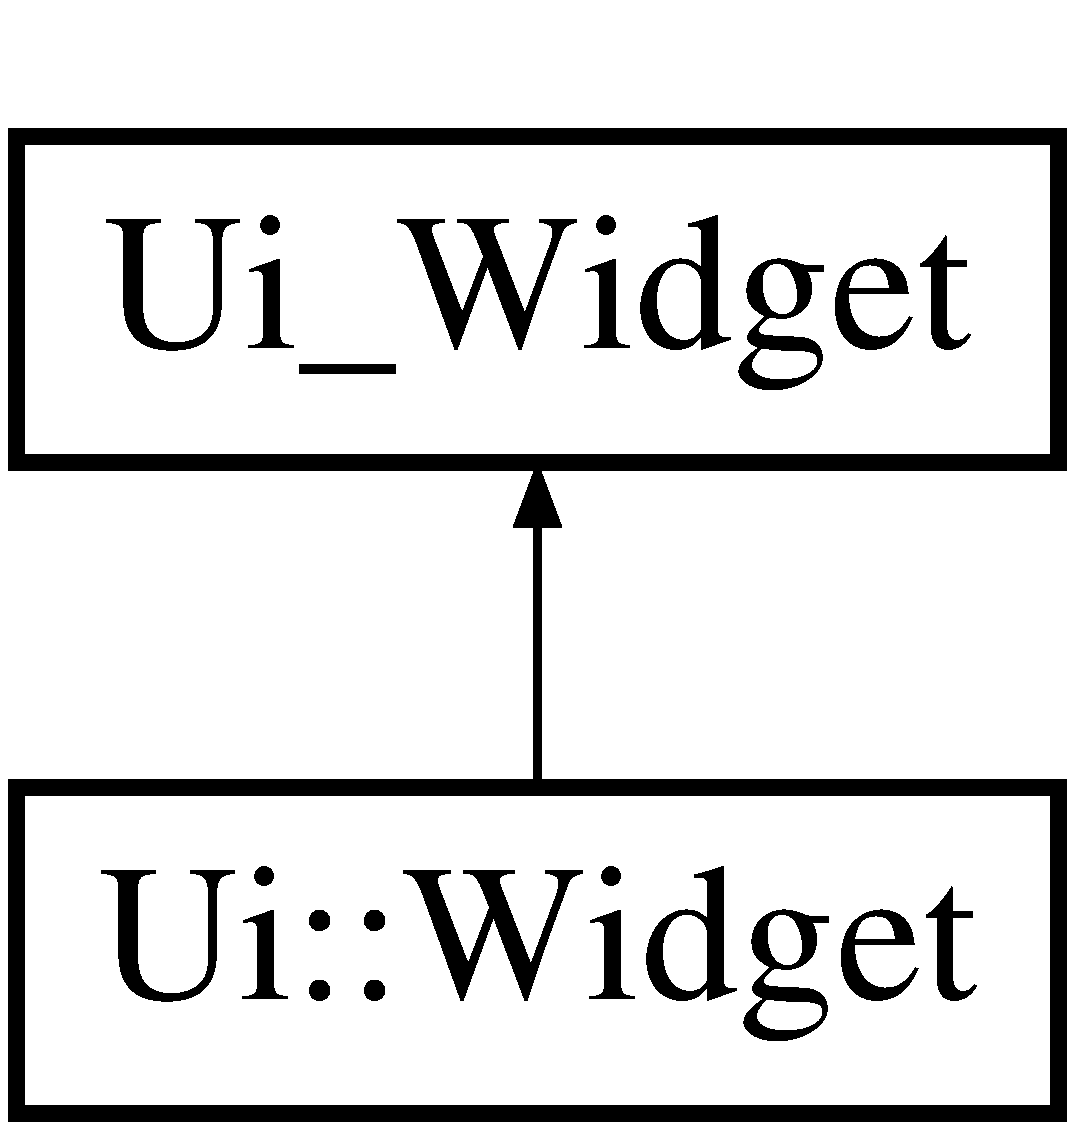
\includegraphics[height=2.000000cm]{class_ui_1_1_widget}
\end{center}
\end{figure}
\subsection*{Additional Inherited Members}


La documentation de cette classe a été générée à partir du fichier suivant \-:\begin{DoxyCompactItemize}
\item 
C\-:/\-Users/\-William/\-Dropbox/lo21/projet/\-Projet/ui\-\_\-onglet.\-h\end{DoxyCompactItemize}

\printindex
\end{document}
